\documentclass[a4paper,english]{report}
\usepackage{algorithm}
\usepackage{algorithmic}
\usepackage[utf8]{inputenc}
\usepackage{babel,duomasterforside}
\usepackage{color}   %May be necessary if you want to color links
\usepackage{hyperref}
\usepackage{subfig}
\usepackage{svg}
\usepackage{listings}

\definecolor{codegreen}{rgb}{0,0.6,0}
\definecolor{codegray}{rgb}{0.5,0.5,0.5}
\definecolor{codepurple}{rgb}{0.58,0,0.82}
\definecolor{backcolour}{rgb}{0.95,0.95,0.92}

\lstdefinestyle{mystyle}{
	backgroundcolor=\color{backcolour},   
	commentstyle=\color{codegreen},
	keywordstyle=\color{magenta},
	numberstyle=\tiny\color{codegray},
	stringstyle=\color{codepurple},
	basicstyle=\footnotesize,
	breakatwhitespace=false,         
	breaklines=true,                 
	captionpos=b,                    
	keepspaces=true,                 
	numbers=left,                    
	numbersep=5pt,                  
	showspaces=false,                
	showstringspaces=false,
	showtabs=false,                  
	tabsize=2
}

\lstset{style=mystyle}

\usepackage{graphicx,wrapfig,lipsum}
\hypersetup{
	colorlinks=true, %set true if you want colored links
	linktocpage=true,     %set to all if you want both sections and subsections linked
	linkcolor=blue,  %choose some color if you want links to stand out
}

\title{Performance tuning Apache Drill on Hadoop Clusters with Evolutionary Algorithms}
\subtitle{Proposing the algorithm SIILCK (Society Inspired Incremental Learning through Collective Knowledge)}
\author{Roger Bløtekjær}

\begin{document}
	\duoforside[dept={Institutt for informatikk},
	program={Informatikk: språkteknologi},
	short]
	\section{Abstract}
		\subsection{Research question}
		How can we make a self optimizing distributed Apache Drill cluster, for high performance data readings across several file formats and database architectures?
		\subsection{Overview}
		Apache Drill enables the user to perform schema-free querying of distributed data, and ANSI SQL programming on top of NoSQL datatypes like JSON or XML - typically in a Hadoop cluster. As it is with the core Hadoop stack, Drill is also highly customizable, with plenty of performance tuning parameters to ensure optimal efficiency. Tweaking these parameters however, requires deep domain knowledge and technical insight, and even then the optimal configuration may not be evident. Businesses will want to use Apache Drill in a Hadoop cluster, without the hassle of configuring it, for the most cost-effective implementation. This can be done by solving the following problems:
		\begin{itemize}
			\item How to apply evolutionary algorithms to automatically tune a distributed Apache Drill configuration, regardless of cluster environment.
			\item How do we benchmark the cluster against default Drill settings to ensure that the algorithm is adding value to the cluster performance, measured as execution time.
		\end{itemize}
		To solve these problems we introduce the evolutionary algorithm SIILCK (Society Inspired Incremental Learning through Collective Knowledge), a development inspired by PBIL \cite{pbil}.
		\subsection{Details}
			\subsubsection{Self optimizing}
			The goal here is that no human intervention is needed to fine tune the Drill configuration. Once the framework / algorithm is executed on the Drill environment, it should only end execution once solution has converged.
			\subsubsection{SIILCK}
			The methodology for self optimization in this thesis is evolutionary algorithms. No current framework or algorithm supported the specific needs for this task, hence SIILCK was developed. The original concept for this thesis used genetic algorithms, then we switched to population based incremental learning (PBIL), ultimately developing SIILCK based on our experience with PBIL. For this thesis SIILCK is used in a tailored application for Apache Drill optimization. However SIILCK itself is an incredibly flexible algorithm, able to solve a wide array of problems through the use of complex structures as candidate solutions, borrowing from techniques used in several independent evolutionary algorithms. More on SIILCK can be read in the method chapter, \hyperref[sec:siilck]{SIILCK}.
			\subsubsection{Distributed file systems / cluster environments}
			Apache Drill can easily be run on any file system, as they are mounted when needed. As such a single node environment is entirely possible to set up, with the local file system mounted as a "Drill Bit". However this thesis focuses on current and future industry standards, and how to optimize Drill in a relevant a big data environment. This is more representative of its intended use, and gives the thesis more value as a research field advancement.
			\subsubsection{ANSI SQL}
			There are similar platforms to Apache Drill, like the popular Apache Spark. Spark also provides SQL querying on data, however this is only a subset of SQL. Only Drill has the full suit of SQL programming capabilities as defines by ANSI (American National Standards Institute), which gives more in depth querying.
			\subsubsection{NoSQL}
			Previously NoSQL databases where known as "Non-SQL" databases, but this has now changed to be "Not Only SQL" databases as they have begun supporting SQL-like querying. The main point about them is that they are non-relational, distributed, open-source and horizontally scalable \cite{no_sql}.
	
	\pagebreak
	\section{Foreword}
	
	I would like to thank my amazing wife Ingrid-Alice Bløtekjær for allowing me to complete this thesis by singlehandedly taking care of our two children - giving me space to perform.
	\\
	\\
	Also a big thank you to my supportive supervisor Anis Yazidi for inspiring me to pursue big data infrastructure, optimization algorithms and autonomy as fields of study - creating the foundation for my career.
	
	\tableofcontents
	
	\chapter{Preface}
	\section{Abbreviations}
	\label{word_list}
	\begin{table}[H]
		\centering
		\begin{tabular}{ll}
			
			DSN & Data Source Name \\
			ER & Entity Relation \\
			GA & Genetic Algorithms \\
			HDFS & Hadoop Distributed File System \\
			JDBC & Java Database Connectivity \\
			MPP & Massively Parallel Processing \\
			ODBC & Open Database Connectivity \\
			OOP	& Object Oriented Programming \\
			PBIL & Population Based Incremental Learning \\
			RPC & Remote Procedure Call \\
			SIILCK & Society Inspired Incremental Learning through Collective Knowledge \\
			SMB & Small / Medium Business \\
			SQL EE & Structured Query Language Execution Engine \\
			TTE	& Time To Execute \\
			
		\end{tabular}
	\end{table}
	\section{Mathematical \& algorithmic annotations}
	\label{table:annotations}
	\begin{table}[H]
		\centering
		\begin{tabular}{ll}
			$P$	& Probability \\
			$P_{mut}$	& Probability for mutation \\
			$P_{i,j}$	& Probability for option \textit{j} in parameter \textit{i} \\
			$i$  & Parameter in a solution \\
			$j$ & Option in a parameter \\
			$i_{j}$ & Active option in parameter \\
			M & Learning rate (amount for mutation to affect the probability vector) \\
			$\mu$ & Academic \\
			$P_{i,j}(t)$ & Probability for option \textit{j} in parameter \textit{i} at time \textit{t} \\
			$\mu_{i,j}(t)$ & Active option \textit{j} in parameter \textit{i} at time \textit{t} for academic $\mu$ \\
			$\beta_{i}$ & Parameters in PBIL collective genetic material \\
			$\varepsilon$ & Resistance
			
		\end{tabular}
	\end{table}

	
	\chapter{Introduction}
		
		\section{Target group}
		This thesis covers the deep technical aspects of big data analysis and evolutionary algorithms - However, all techniques used will be explained in detail. Computer science students looking into infrastructure or biologically inspired programming will probably feel the most at home, in terms of discussed concepts and technical terms. For the layman, there is also a \hyperref[word_list]{list of abbreviations} supplied.
		
		\section{Area of research}
		Hadoop and MapReduce are already well established technologies employed in countless applications around the world, Apache Drill however is a fairly new concept with little to no research from the community. We propose a new method of implementing Hadoop clusters with Apache Drill, automatically optimizing the performance tuning in a lightweight and low effort way. As such this is partly a technical thesis regarding performance tuning, and the implementation aspects of an Apache Drill cluster. The other part covers the evolutionary algorithm developed.
		
		\section{Research question - in full}
		\subsection{Goal, justification and challenges}
		The goal for this thesis is to optimize an SQL Engine called Apache Drill that sits on top of a distributed file system, for more cost-effective big data handling, business intelligence and advanced analytics. Businesses that handle big data will most likely perform plenty of queries every day, or even every hour. If we were to add up the amount of time spent waiting for a query to complete, for a year, and converted the hours into money - we would find it costs a lot of money to convert raw data into information. That's why saving even 1\% in execution time can mean a difference when it comes to overhead costs. So naturally there is a massive amount of research for improving execution time and other metrics, even more so when it comes to shared computing like cloud services where you pay by the minute. The SQL Engine chosen here is Apache Drill, a fairly new framework inspired by Google Dremel, and currently the only schema-free engine to run directly on top of HDFS, allowing users to drill into complex data like JSON. Looking to for example Yelp, we can see that their entire database is available as JSON \cite{yelp}, allowing for far more complex  and flexible handling of metrics than conventional ER databases. As with the other data handling engines on distributed storage platforms, there are many parameters to consider if one wants to increase performance - in fact so many that it is considered infeasible without in depth expertise of domain and engine. Considerations are:
		\begin{itemize}
			\item Type of storage (distributed or single node)
			\item Amount of computing nodes (cluster or not)
			\item Size of nodes (memory and CPU)
			\item Type of data (complex or not)
			\item Size of data (few large files or plenty small ones)
			\item Distribution of data (heavy skew or uniform distribution)
			\item Execution engine specific parameters (for which there are many)
		\end{itemize}
		All of these parameters work in tandem to produce a measurable performance. That's why genetic algorithms was chosen as a tool for self optimization, to take all of these parameters into consideration automatically - and simply test solutions until converging into a good one (considered optimal). Some of the parameters are statically set in this thesis, such as cluster size, to simulate a SMB environment, and to have some testing grounds. There would be no alterations needed to apply the methods presented in this thesis in either an enterprise with 1000 clustered nodes, or a single laptop, but for the sake of argument we mimic a real world use case.
		\subsection{Resarch question}
		How can we make a self optimizing distributed Apache Drill cluster, for high performance data readings across several file formats and database architectures?
		
		\section{Personal motivation}
			\subsubsection{Subject}
			The subject for this master thesis is a natural continuation of our previous work \emph{Hadoop MapReduce Scheduling Paradigms}, published in 2017, in the 2nd IEEE International Conference on Cloud Computing and Big Data Analysis \cite{own}. Back then the topic was haphazardly picked from a list of eligible ones, but the more we read into it - the more we understood the incredible use cases for Hadoop within the massive industries that are driving forces for our technological advancements. As is common in IT, levels of abstraction get added on top of proven technologies both to make implementation better, and often to increase performance. Since then Apache Drill has seen plenty of stable builds and proven itself to be potentially industry-changing in the way we handle our data - entering a schema-on-the-fly paradigm.
			
			\subsubsection{Apache Drill as a platform}
			As mentioned previously there is little to no research done on Apache Drill as a platform. Some of the reasoning might be the that some still considers it to be in the early development phase, but as of this writing there has already been one major release, \textbf{1.0} in 2015, and 12 subsequent minor releases up till \textbf{1.12} \cite{drill_releases}. So we would argue the project is past the early development phase, and moving into the early adopter phase. But why choose to use this platform over more established ones, and what other options are there? This is discussed further in a following section: \hyperref[sec:why_drill]{Why is this worthwhile?}
			
		
		\section{Research method in brief}
		Throughout this thesis we will develop an entire suite of tools centered around an evolutionary algorithm for automatically optimizing Apache Drill on top of a Hadoop cluster, tested on big and diverse sample sets. As the framework is expected to change, all of the parameters tweaked will be in relation to the current Apache Drill version being used, \textbf{1.12}. The main goal is to achieve a performance increase, measured as TTE (Time to Execute) for single and/or concurrent queries.
		
		\section{Most relevant previous findings}
		There is little to no research done on the impact of tuning Apache Drill. However, tuning of parameterized frameworks have been done a lot in the past on industry standards like SQL, MySQL, traditional Hadoop clusters (mapreduce scheduling algorithms), and Web applications. Since Apache Drill has its own SQL execution engine,  the tuning of SQL systems in previous works has value for how we will benchmark our Drill perfomance.
			\subsection{Starfish}
			Herodotos et al made on of the most cited papers in the Hadoop research field, when they proposed Starfish \cite{starfish}. Starfish is a self-tuning system for Hadoop clusters, citing the lackluster performance of default cluster parameters to be the motivation. They designed a modular system where the main parts include:
			\begin{itemize}
				\item A profiler that analyzes jobs and determines cost estimation and the data flow.
				\item A novel approach to predictive tuning they named the "what-if-engine". It's job is to predict how different parameter configuration tweaks will change the performance of the system.
				\item A cost-based optimizer, that performs the pure tuning aspects, based on estimations from the what-if-engine.
			\end{itemize}
			Our project has very similar goals and motivations compared to this project, except on a framework on top of Hadoop, instead of directly on it.
		
		\section{Why is this worthwhile, why Drill?}
		\label{sec:why_drill}
			\subsection{Ease of use}It is safe to say that information technology as a subject is only getting more popular by demand. According to projections made by renown recruitment company Modis, tech employment will see a 12\% growth by 2024, vs 6,5\% in all other industries\cite{modis}. This means that a lot of new engineers will enter the workforce, and start building and maintaining enterprise applications. Apache Drill serves a very low barrier of entry for newcomers with its' SQL ANSI queries when handling big amounts of data, as opposed to i.e the popular Java Enterprise framework Persistence. Using Apache Drill will therefore require less training, thus increasing productivity and agility in young teams.
			\subsection{Increasing relevance of Big Data infrastructures}
			\label{big_data}
			\textit{"From 2005 to 2020, the digital universe is expected to grow dramatically by a factor of 300, from 130 exabytes to 40 trillion gigabytes, i.e more than 5,200 gigabytes per person in 2020. Moreover, the digital universe is expected to double every two years"} \cite{bigdata}.
				\subsubsection{Real time data usage}
				Successful digitalization of businesses often require applications to utilize data in real time, serving customers relevant data instantaneously. \textit{"Now, most applications are generating real-time data, so superfast data capturing and analysis within a fraction of a second are mandatory"} \cite{management_analytics}.
				\\
				An interesting example of this is chat applications (instant messaging). Users of messaging apps today expect it to store data indefinitely, and deliver instant communication between users, creating an absolutely enormous global data flow. Bettercloud.com performed a study and found that \cite{bettercloud}:
				\begin{itemize}
					\item The majority of organizations (57\%) use two or more real-time messaging applications.
					\item 80\% of Skype for Business users, 84\% of Google Hangouts users, and 95\% of Slack users say communication has improved because of real-time messaging.
					\item 56\% of respondents believe that real-time messaging will displace email as their organization’s primary workplace communication and collaboration tool.
				\end{itemize}
				From these results we see that adoption of applications using real time data is only increasing. This will provide a future need for fast and scalable infrastructure to cope with it. 
				\subsubsection{Combining real-time and stored data}
				In reality a lot of current applications that create value combine the usage of analytics on stored data and real-time sensor data. Predictive maintenance is an example of a discipline where you analyze historical data, finding thresholds and patterns for when components in a system break down, and then combining this knowledge with real time sensors to service the components before they fail. This saves money on planned maintenance where healthy parts get serviced, and downtime on systems where they have to be set aside for the service. In a Harvard Business Review on a company called \textbf{Servicemax} that has specialized in services like this they wrote that:
				\textit{"(...) customers, on average, increase productivity by 31\%, service revenue by 14\% and customer satisfaction by 16\%"} \cite{servicemax}. All of this is empowered by big data, and the utilization of information.
			
			\subsection{Application needs}
			\begin{figure}[H]
					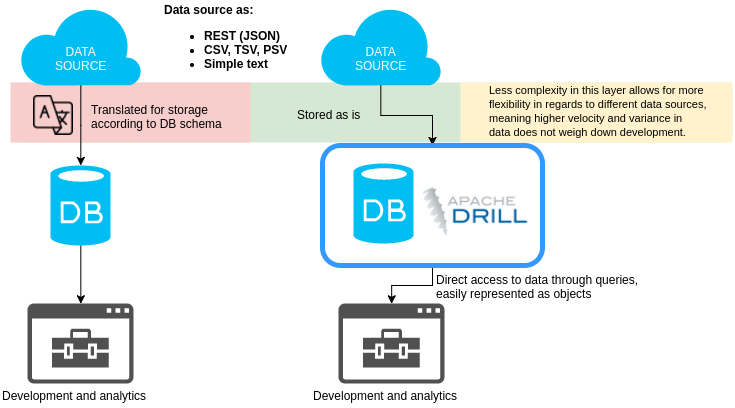
\includegraphics[width=\textwidth]{drill_advantages}
					\caption{Advantages of schema-free querying}
			\end{figure}
			\textit{"Object and relational technologies are grounded in
			different paradigms. Each technology mandates that
			those who use it take a particular view of a universe
			of discourse. Incompatibilities between these views
			manifest as problems of an object-relational
			impedance mismatch"} \cite{impedance}.
			\\
			Traditional databases contain tables (entities) with relations between them. Sometimes these systems consist of thousands of tables, even going as far as tens of thousand (like this database of the human genome with 20000 tables \cite{humangenome}). Object-oriented programming classes is difficult and oftentimes inefficient to map directly to the raw data. Especially when there are large amounts of data, it can take a while just initializing the objects, and then again when serializing them to store them. Adopting complex storage file types like JSON for raw data would overcome this mismatch, and allow for more agile, and reactive development of enterprise applications utilizing huge data sources. The global IT industry is increasingly transitioning to deliver RESTful APIs to their customers. With Apache Drill, it is extremely easy to perform queries on the results, even joining them against several other data sources or combining results from several APIs at the same time, in real time. For application developers this will eliminate the middleware of a relational database, having to translate the data for different purposes. Instead of having one format for storing, one for interfacing and one for application logic, Apache Drill and the schema-free paradigm will provide one single interface for all dimensions of data.
		
		\section{How far will this advance the field?}
			\subsubsection{Advances in research}
			The ambition for this project is to provide a fully functional, open source light weight framework allowing companies to easily deploy Hadoop Clusters with Apache Drill without worrying about tailoring the solution or suboptimal performance. In terms of research, this is the first thesis written about performance tuning of Apache Drill, and as such will lay a foundation for the future of this field.
			\subsubsection{Advances in industry}
			As the previous section highlighted (\hyperref[big_data]{Increasing relevance of Big Data infrastructures}), we predict an increase in future global data collection, going as far as doubling the amount of data per person, per year. This data is only collected to add value to a business, and the revenue increase for businesses that embrace big data analytics will not go unnoticed by the industry, leading to wider adoption. Some businesses already make huge profits simply by gathering and selling information, like Google and Facebook, increasing their yearly revenue since 2011 by 289\% and 1095\% respectively \cite{statista}. Data is becoming the world’s new natural resource \cite{future_data}. To be able to more fluidly handle this data in applications, we believe agile teams will want flexible frameworks that empower more cost effective development and big data utilization. When the industry realizes Apache Drill can deliver that, this will lead to a paradigm shift to schema-free querying of data, and on-the-fly data reads without tailoring.

		
	\chapter{Background}
	\emph{"Apache Drill is one of the fastest growing open source projects, with the community making rapid progress with monthly releases. The key difference is Drill’s agility and flexibility. Along with meeting the table stakes for SQL-on-Hadoop, which is to achieve low latency performance at scale, Drill allows users to analyze the data without any ETL or up-front schema definitions. The data can be in any file format such as text, JSON, or Parquet. Data can have simple types such as strings, integers, dates, or more complex multi-structured data, such as nested maps and arrays. Data can exist in any file system, local or distributed, such as HDFS or S3. Drill, has a “no schema” approach, which enables you to get value from your data in just a few minutes"} \cite{drill}.
	
	\section{History}
		\subsection{Creation and adoption of Hadoop}
		Google created the Google File System in 2003 \cite{gfs}, predicting the paradigm of distributed storage. Then, the MapReduce concept for sorting / counting data was added in 2004 \cite{mapredoriginal}. Hadoop was introduced as a platform in 2006 \cite{hadoopguide}, and together with MapReduce, it made an impact in the industry, attracting talent and big companies eager to contribute and deploy. Yahoo was a big early adopter, being one of the first companies deploying big clusters as early as 2006 \cite{hadoopguide}. Then in 2008, Hadoop got the world record for fastest system to sort a terabyte of data \cite{hadoopguide}. After this, development accelerated with more contributers and interest was at an all time high. Since that point in time Apache Hadoop has become the most widely used platform for Big Data handling, empowering advanced analytics and business intelligence across several industries. The Hadoop stack is now highly scalable, ensures high availability of data, and utilizes parallel processing to deliver high performance data readings.
		
		\subsection{Google branching out with Dremel}
		In 2010 Google did further research on distributed data processing and published their paper on Dremel \cite{dremel}. Dremel is the framework that empowers Google's current platform Google BigQuery, delivered as Infrastructure as a Service (IaaS). Among customers of BigQuery is well recognized brands like Spotiy, Coca Cola, Philips, HTC and Niantic \cite{dremelcustomers}. The success of Google BigQuery (by extension of Dremel), inspired Apache to create Drill, the framework being examined in this thesis.
	
	\section{Technology}
	\label{technology}
		
		\subsection{Hadoop stack}
		
		\subsubsection{Hadoop common}
		Hadoop common consists of a few select core libraries, that drives the services and basic processes of Hadoop, such as abstraction of the underlying operating system and file system. It also contains documentation and Java implementation specifications. 
		
		\subsubsection{HDFS}
		HDFS (Hadoop Distributed File System) is a highly fault tolerant, distributed file system designed to run efficiently, even on low-cost hardware. HDFS is tailor made to express large files and huge amounts of data, with high throughput access to application data and high scalability across an arbitrary amount of nodes.
		
		\subsubsection{YARN}
		YARN (Yet Another Resource Negotiator) is actually a set of daemons that run in the cluster to handle how the jobs get distributed. 
		\begin{itemize}
			\item There is a NM (NodeManager) that represents each node in the cluster, monitoring and reporting to the RM whether or not they are idle, and resource usage (CPU, memory, disk, network). A node in a Hadoop cluster divides its resources into abstract Containers, and reports on how many containers there are available for the RM to assign jobs to.
			\item There is an AM (ApplicationMaster) per job, or per chain of jobs, representing the task at hand. This AM gets inserted into containers on nodes, when a job is running.
			\item Finally there is a global RM (ResourceManager), which is the ultimate authority on how to distribute loads and arbitrate resources. The RM consists of two entities, the Scheduler and the ApplicationsManager.
			\begin{itemize}	
				\item The ApplicationsManager is responsible for accepting job submissions (at this point represented as an ApplicationMaster), i.e by doing code verification on submitted jobs, changing their status from "submitted" to "accepted". Once a job is accepted, the ApplicationsManager sends the ApplicationMaster to the scheduler to negotiate and supply containers for the job on the nodes in the cluster. The ApplicationsManager also has services to restart failed ApplicationMasters in containers, and retry entire jobs.
				\item The Scheduler is a pure scheduler in the sense that it only cares about delivering tasks to idle slots, based on free resources on the node. It calculates distributions across multiple nodes / containers, and can prioritize - i.e compute smaller jobs in front of large ones to more effectively complete job queue, even though the large job was submitted first. The Scheduler does not care for monitoring task completions or failures, simply distributing loads on the cluster.
			\end{itemize}
		\end{itemize}
		\textit{The ResourceManager and the NodeManager form the data-computation framework. The per-application ApplicationMaster is, in effect, a framework specific library and is tasked with negotiating resources from the ResourceManager and working with the NodeManager(s) to execute and monitor the tasks} \cite{yarn}.
		
		\subsubsection{MapReduce}
		MapReduce is the heart of a traditional Hadoop cluster, for which every other component is built around, to maximize its efficiency. It is a model for distributed processing of big data, to process and consolidate. It is defined by two stages - the mapping phase, and the reduce phase. Both of these phases require resources from the node it is run on, defined by a set amount of map slots and reduce slots. The amount of slots on a node for each task is parameterized and can be set by an administrator / or typically algorithmically. The map phase consists of parallel map tasks, that map a key to a value. All of these map tasks then consolidate into the reduce phase, where they are combined so that one key exists for all accumulated values. So for instance if we're counting cards in several decks across several nodes, they would each map something like "(Queen of Hearts, 1)". In the end the reduce task consolidates all these single queens, so it ends up looking like "(Queen of Hearts", 27)". This is a far more effective approach than for instance looping through all the decks and incrementing a key by one for each matching key we find. Especially when the data that typically gets handled by a Hadoop cluster is diverse and hard to predict.
		
		\subsection{Zookeeper}
		Zookeeper is not a part of the Hadoop core utilities, but is is often to be found in Hadoop clusters. It is used as a distributed storage platform for configuration information, synchronization and naming. While YARN handles the distribution of tasks between the nodes in the cluster, Zookeper takes care of failover, race conditions and sequential consistency. This tool looks more like orchestration frameworks such as Puppet or Chef, in that it organizes the amount of YARN nodes and distributes configurations, availability and atomicity.
		
		\subsubsection{Zookeeper Quorum}
		Even though Zookeeper is made as a distributed configuration management and failover safeguard, it can be installed on a single node. Running Zookeeper in this way is called a Standalone Operation, and give a user a interface to remotely connect to, to get some data on running services etc. However, we need Zookeper distributed across all our nodes. This is called a Quorum. In a Quorum, every node will check the health of the others. If there is a consensus among nodes that one is down, Zookeeper is able to communicate this to YARN, letting it distribute loads across the remaining healthy nodes. 
		
		\subsection{Apache Drill}
		In this thesis there won't be any in-depth explanations of the inner workings or architecture of Drill, but we'll gloss over the broader picture in this section.
		\subsubsection{What is it}
		Apache drill is the newest technology to be introduced in this chapter. All the previously mentioned frameworks are tried and tested - proven over time. Apache drill rests on top of all these technologies, and provides a way to query almost any non-relational database. This means that we can set up a cluster on a data lake with a very diverse data type, and still perform standard ANSI SQL queries on it. Even in formats like JSON, a simple SQL query can provide all the insights one might need. Apache Drill is inspired by Google Dremel, which as mentioned is the driving force behind their advanced Big Data Analytics tool - Google BigQuery. Apache Drill is a SQL EE for MPP, that works in almost any environment and on almost any file type. Whether querying complex data, text files or entire directories of log files, Apache Drill allows for standard SQL interfaces for reading the data.
		\subsubsection{How does it do it}
		\paragraph{The drillbit}
		In its core Apache Drill simply consists of a Daemon service called a Drillbit. The drillbit can be installed on any server or client device that has data, or on any number of nodes within a Hadoop cluster, to perform SQL queries. This means that Drill is an entirely independent piece of software, able to perform its intended task without any environment specific needs. Thus Drill does not use YARN, and simply uses hadoop for the distributed storage. To run MPP in a cluster however, Drill is dependent on Zookeeper.
		\paragraph{Querying drill} In addition to its flexible installation needs, the query inputs to Drill can come from a wide variety of sources - JDBC, ODBC, a REST interface, and from a C++ or Java API.
		\paragraph{Key components}
		\begin{itemize}
			\item An RPC end point to receive queries and communicate with clients
			\item An SQL parser that interprets the SQL input and outputs a logical plan
			\item An optimizer that takes the logical plan and translates it to a physical plan based on data locality and node resources
			\item A storage engine interface that has the ability to mount any type of storage, from a local hard drive to a distributed storage like HDFS
		\end{itemize}
		\begin{figure}[H]
			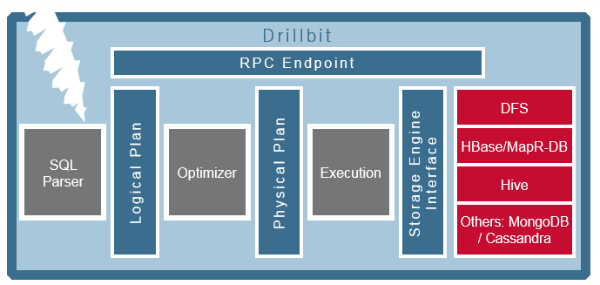
\includegraphics[width=\textwidth]{mapr_drill1}
			\caption{Drill components \cite{mapr_drill}}
		\end{figure}
	
		\paragraph{Drill in a cluster}
		When using Drill as an SQL EE in a distributed storage, it is highly recommended to install a drillbit on all nodes. When set to perform MPP drill is dependent on Zookeeper to keep track of all the drillbits.  When a query is submitted, the first node to respond to the initial request from Zookeeper becomes the \textit{Foreman}. In Drill there is no master or slave hierarchy, and for every query submitted a new foreman is selected. Every drillbit contains all services and capabilities of Drill, which makes it highly scalable - just add another node and install Drill and you're done (after adding it to the Zookeeper Quorum). The foreman gets a list of available Drillbit nodes in the cluster from ZooKeeper, and determines the appropriate nodes to execute various query plan fragments to maximize data locality. This means that Apache Drill both performs the planning, distribution and execution of queries, only depending on Zookeeper to keep track of available nodes. Once a foreman has decided on the distribution of the query, the workload gets split downwards into fragments to the nodes, and the results get consolidated upwards until reaching the foreman, which then returns the results to the client.
		
		\begin{figure}[H]
			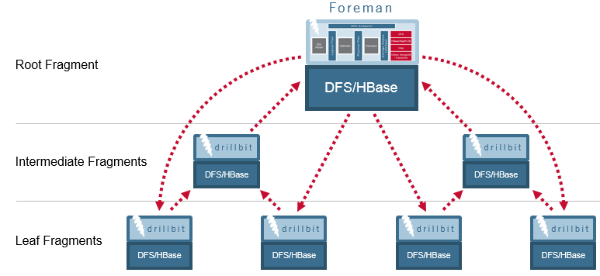
\includegraphics[width=\textwidth]{mapr_drill2}
			\caption{Drill parallel processing \cite{mapr_drill}}
		\end{figure}
		
		\subsection{Drill ODBC Driver, and unixODBC}
		To be able to programatically perform queries to the Drill cluster we need an interface to connect to. This is done via a Open DataBase Connectivity (ODBC), that is installed on the NameNode of the Hadoop cluster. unixODBC is the self-proclaimed definitive standard for ODBC on non MS Windows	platforms \cite{unixodbc}. Once unixODBC was set up, the Drill ODBC Driver was installed on a arbitrary drillbit, although we chose the Hadoop NameNode for this as well. This then allows for setting up a Datasource referencing the Zookeeper Quorum which can then be contacted programmatically, interfacing Drill as if it were a standard SQL server / database.
		
		\subsection{pyodbc}
		There are plenty of ways to interface with an ODBC. We chose python as a preferred language because of familiarity. Therefore we chose to use pyodbc \cite{pyodbc} to communicate with the ODBC, allowing a fully functional interface against our Drill configuration. pyodbc is a well established open source module, implementing the DB API 2.0 specification which is an API defined to encourage similarity between the Python modules that are used to access databases. Defining the Drill ODBC Driver as a datasource, which again points to the Zookeeper Quorum, proved effortless and fast.

		\section{Genetic algorithms}
			\begin{figure}[H]
				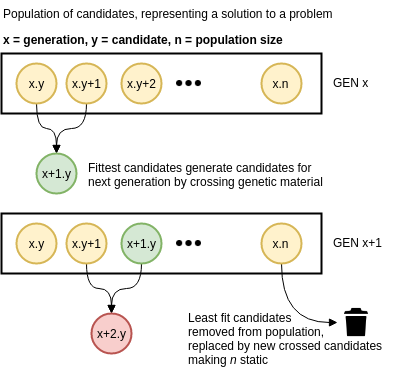
\includegraphics[width=\textwidth]{GA}
				\caption{Basic concepts of GA}
			\end{figure}
			Genetic algorithms are higher level procedures for generating high-quality configurations / solutions to problems with a wide range of parameters, typically where exhaustive searches are infeasible. The procedure starts out with a population of \textit{n} candidates, each representing a set of pseudo-randomly generated values for the respective parameters (properties) that will yield a result for the given problem. Once each candidate has attempted to solve the problem by applying their properties to it, a fitness score is given and compared amongst them. The fitness score represents how good their solution to the problem was, and lets us pick out the best candidates among our population. After the optimal candidates of a generation is chosen, a new generation is generated, inheriting the properties of the previous best candidates. This process repeats until a stop criterion is reached and the properties of the candidate is considered an optimal solution. The number of generations to be generated, and the number of parent candidates from which the next generation is generated from are tweakable parameters.
			
			\subsection{NASA applying genetic algorithms}A very famous application of genetic algorithms is the high-performance antenna NASA made, that actually flew in their Space Technology 5 (ST5) mission \cite{nasa}. In NASAs case, they needed to make a highly receptive antenna with very small physical dimensions. It could have any number of branches, each going in any arbitrary direction. Because of these seemingly infinite possible configurations for the antenna, applying genetic algorithms to gradually evolve a design by testing randomly generated populations and combining the best traits from each candidate, proved to be a great way of solving this. \emph{"(...) the current practice of designing antennas by hand is severely limited because it is both time and labor intensive and requires a significant amount of domain knowledge, evolutionary algorithms can be used to search the design space and automatically find novel antenna designs that are more effective than would otherwise be developed"} \cite{nasa}.
			\clearpage
			\subsection{Limitations of genetic algorithms}
			\subsubsection{Fitness function}
			At first glance it sounds like applying genetic algorithm techniques to any problem would yield an optimal solution, with relative ease. The problem though, is the fitness function for determining the candidate solution. As the complexity of the problem scales in size the search space for the fitness function will end up being too big to complete in a reasonable time. For instance if one single candidate evaluation took days, performed for the whole population, across generations, it could end up taking months completing just one single optimization. In those cases machine learning approaches or simply manual labor through technical and domain specific knowledge would prove to be more efficient.
			\subsubsection{Reaching the optimal solution}
			The only way to evaluate a solution is to compare it against other solutions within the population, all of which have are derived from random mutations. Therefore it is impossible to know whether a truly optimal solution is reached, or if one more generation of mutations will prove to give a better result. In practice a stop criterion for the candidate generation is therefore needed, where a solution is considered to be optimal.

	\pagebreak
	\section{Population based incremental learning}
	\begin{figure}[H]
		\centering
		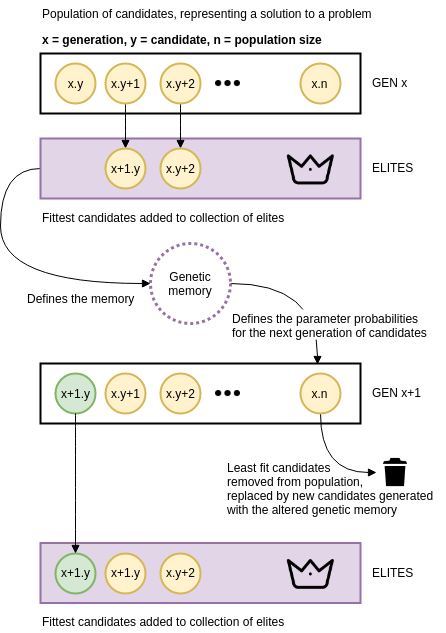
\includegraphics[width=310pt]{PBIL}
		\caption{Basic concepts of PBIL}
	\end{figure}
	The distinction between PBIL and the general GA lies in where the evolution happens. GA generally focus on evolving individual candidates, and crossing fit parents to produce extra fit children, each of them with a chance of mutation. Across several generations convergence is expected. PBIL on the other hand evolves the whole population on a higher level, where the probability vector for parameter generation is shifted towards a considered favorable state. So instead of generating new candidates defined as a crossover function of two parents, the fittest candidates affect a shared genotype that each candidate is generated from. This allows for a much clearer convergence of properties, where you end up in a state where every parameter has a (close to) 100\% chance to be generated. This approach was first proposed back in 1994 by Baluja, where he found that \textit{"The results achieved by PBIL are more accurate and are attained faster than a standard genetic algorithm, both in terms of the number of evaluations performed and the clock speed. The gains in clock speed were achieved because of the simplicity of the algorithm"} \cite{pbil}.
	\section{SIILCK}
		\subsection{Based on PBIL, built for speed}
		While PBIL directly mutates the collective probability vector without testing the mutation, SIILCK avoids unnecessary mutation on key properties by only altering the collective probability vector in the case of a beneficial mutation. In the case of Apache Drill there are a number of boolean properties that have big impacts on performance, i.e "planner broadcast join" that based on setting can result in a query that is \textit{"(...) substantially cheaper"} \cite{joinplanning}. The impact of flipping this boolean property is based on the type of query being done, the skewness of data locality and cluster size, but for a specific type of query in a set environment the property will always have a strictly optimal value. In SIILCK this will become apparent early, and the chance of this value being anything else than the optimal one is likely decreased instantly after first generation has ran its jobs, and in every subsequent generation. Typically this will result in a snowballing effect, where crucial parameters quickly get favored, further increasing the chance of them being selected, accelerating the selection process. Further more SIILCK allows for complex values as genetic material instead of the usual binary representation of GA and PBIL, making it easier to implement linear parameters. A shared genetic memory that PBIL first introduced, (here called the collective knowledge), for the population also matches well with the method presented in this thesis - of measuring performance of the candidate parameters on the SQL EE with an authority object. This is further detailed in the method chapter, \hyperref[sec:society]{society}.
		\pagebreak
		\subsection{Limitation of SIILCK}
		The main advantage of SIILCK is also its main limitation, that each candidate property needs a preset of developer defined values. Thus finding the optimal solution is still based widely on the amount of options, and the effectiveness of them, defined by the developer of the algorithm. Naturally - in terms of boolean properties there lies no challenge. However when linear parameters need to be set, i.e properties with ranges from zero to infinity, the developer must define a set of valid options existing within that range. In the context of Apache Drill there are default rule of thumb values for each property, so the list of valid options for each property is generated around the default. Another drawback of SIILCK, as with many evolutionary algorithms, lies in the risk of premature convergence. This can however be mitigated by effective mutation functions that ensure diversity.
	\pagebreak
	\section{Related literature and theoretical focus}
		\subsection{Performance tuning MapReduce as a Research Field}
		There is a ton of research to be read about MapReduce optimization, trying to tune map- and reduce-slots, and improve the inherent job tracker. Looking at a few essential papers within this field shows a general consensus that tuning default performance parameters in a variety of environments will lead to 10-30\% performance increase, which naturally results in considerable cost savings. For instance Min Li et. al. could report that "\textit{Our results using a real implementation on a representative 19-node cluster show that dynamic performance tuning can effectively improve MapReduce application performance by up to 30\% compared to the default configuration used in YARN}" \cite{mronline}. Furthermore, manually tuning these clusters are too demanding for most businesses to even consider, requiring both deep technical and domain-specific insight. These findings further maintain our vision of bringing auto-tuning to the Apache Drill framework, which we believe to be the next natural step forwards, even paradigm-defining, for big data handling.
	
		\subsection{Mapreduce optimization}
			\subsubsection{Gunther}
			Gunther evaluated methods for optimizing Hadoop configurations using machine learning and cost-based models, but found them inadequate for automatic tuning. Thus they introduced a search-based approach with genetic algorithms, designed to identify crucial parameters to reach near-optimal performance of the cluster \cite{gunther}. This paper tells us that genetic algorithms as an approach to performance tune big data clusters already is a proven method. However, the scope is set to Hadoop as an out-of-the-box enterprise solution, whereas we take the next step within the schema-on-the-fly paradigm of Apache Drill.
			
			\subsubsection{mrOnline}
			"MapReduce job parameter configuration significantly impacts
			application performance, yet extant implementations place the bur-
			den of tuning the parameters on application programmers. This is
			not ideal, especially because the application developers may not
			have the system-level expertise and information needed to select
			the best configuration. Consequently, the system is utilized inefficiently which leads to degraded application performance" \cite{mronline}.
			
		\subsection{Other Hadoop SQL engines}
		There are plenty of SQL-on-hadoop engines available right now, like CitusDB, Impala, Concurrent Lingual, Hadapt, InfiniDB, JethroData, MammothDB, Apache Drill, MemSQL or Pivotal HawQ, and the amount of independently developed engines speaks volumes of the interest in this field. Why Apache Drill was chosen in this thesis is detailed in the \hyperref[sec:why_drill]{Why Drill section}, but the fact that Drill is (at the time of this writing) the only schema-free engine is a major selling point. However Impala and Spark are often considered as alternatives in similar environments.
			\subsection{Impala}
			Impala, developed by Apache is an open-source SQL engine that was designed to bring parallel DBMS technology to the Hadoop environment \cite{impala}. The main idea is shared between Drill and Impala where they both set up daemons on each node of a distributed cluster, to perform MPP (Massively Parallel Processing) for data reads, circumventing MapReduce. Impala is made for Big Data Analytics, priding itself in having \textit{"order-of-magnitude faster performance than Hive"} \cite{impalasite}.
			\subsection{Spark}
			Apache also developed Spark, a popular open-source platform for large-scale data processing that is	well-suited for iterative machine learning tasks \cite{spark_ml}. Spark is built with Hive, and runs very similarly to MapReduce but also has extended functionality. The key difference is that Spark keeps things in memory, while MapReduce keeps shuffling data in and out of disk. This allows Spark to facilitate machine learning algorithms on top of big data clusters, reading and processing data in the same work flow
			
	\section{Presentation of domain where technology is used}
		The field of big data analytics is now becoming nigh impossible to ignore for enterprises dealing with customer information. Within this field Hadoop is currently the biggest platform. SiliconANGLE wrote a 5 year future broadcast in 2012, stating that \textit{"Hadoop-MapReduce solution [will] be the de-facto industry standard for business intelligence and projects a 58\% compound annual growth rate"} \cite{siliconA}.
		Global Knowledge Training highlights some of the reasons why Hadoop is seeing such success and adoption rate
		\textit{"It's becoming clear that the open-source Apache Hadoop platform changes the economics and dynamics of large-scale data analytics due to its scalability, cost effectiveness, flexibility, and built-in fault tolerance. It makes possible the massive parallel computing that today's data analysis requires"} \cite{globalknowledge}.
		Further more BMC Software lists industries and sectors where Hadoop is currently being utilized to gain a competitive advantage, increase customer satisfaction or even improve citizen health:
		\begin{itemize}
			\item Financial services companies use analytics to assess risk, build investment models, and create trading algorithms; Hadoop has been used to help build and run those applications \cite{bmc}.
			\item Retailers use it to help analyze structured and unstructured data to better understand and serve their customers \cite{bmc}.
			\item In the asset-intensive energy industry Hadoop-powered analytics are used for predictive maintenance, with input from Internet of Things (IoT) devices feeding data into big data programs \cite{bmc}.
			\item Telecommunications companies can adapt all the aforementioned use cases. For example, they can use Hadoop-powered analytics to execute predictive maintenance on their infrastructure. Big data analytics can also plan efficient network paths and recommend optimal locations for new cell towers or other network expansion. To support customer-facing operations telcos can analyze customer behavior and billing statements to inform new service offerings \cite{bmc}.
			\item There are numerous public sector programs, ranging from anticipating and preventing disease outbreaks to crunching numbers to catch tax cheats \cite{bmc}.
			Hadoop is used in these and other big data programs because it is effective, scalable, and is well supported by large vendor and user communities \cite{bmc}.
			\item Hadoop is a de-facto standard in big data \cite{bmc}.
		\end{itemize}
	
		Now it may seem like the Hadoop platform is an all-encompassing 
		technology when businesses wants to deal with big data. There are however some bleaker recent reports stating that Hadoop adoption is going slower than previously predicted. A 2015 Gartner press release stated that \textit{"[the] future demand for Hadoop looks fairly anemic"} \cite{Gartner}. The reasons businesses aren't adopting Hadoop as a big data framework however was fairly coherent, and is also highlighted in this thesis. It is too technically demanding to set up effectively. Companies that were reluctant or hesitant with Hadoop adoption cited skills shortage and user-unfriendliness as reasons for not thinking about Hadoop \cite{Gartner}. This is the exact reason why self optimizing frameworks like the one introduced in this thesis are needed. Making the Hadoop platform more approachable through a "out-of-the-box" mindset could potentially severely lower the threshold for taking a leap into big data. Through the methods presented in this thesis, we try to directly tackle this problem.
	
	\chapter{Method}
	\label{chap:method}
		
		\section{Infrastructure}
			To simulate a enterprise environment we set up a cluster consisting of four nodes, each with the same spec - 4 VCPUs and 8GB RAM. These were all VMs in OpenStack, each running Ubuntu 17.10. The cluster is also listed in the appendix, called the \hyperref[table:cluster_shared]{shared cluster} The gateway has a outward-facing network interface for SSH access, and from there each of the other nodes can be managed. They all had Apache Drill installed, and were set up as a Hadoop cluster running HDFS between them. All data that Drill uses to read for tests are replicated three times in the cluster, ensuring parallel processing.
			\begin{figure}[H]
				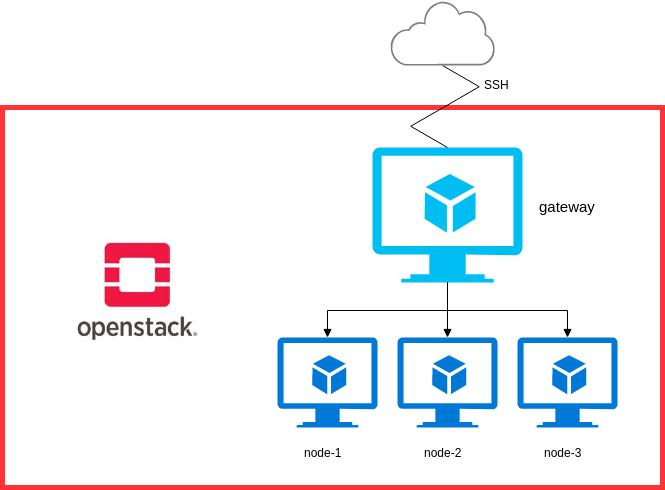
\includegraphics[width=\textwidth]{cluster}
				\caption{Cluster architecture}
			\end{figure}
			The infrastructure stack consists of the technologies listed in the \hyperref[technology]{technology section}. All technologies are installed on all machines, except for the ODBC drivers, that are exclusively on the gateway. During a drill execution, any node can act as the orchestrator, named the \textit{foreman}. On each machine there is a user named \textit{hadoop}, that runs all the services needed to keep the cluster operational, like the zookeeper server and the drillbits. The gateway also has a main user simply named \textit{ubuntu}, that runs the tests and the algorithm. The drillbits are made available through a ODBC DSN.
			The services are as follows:
			\begin{itemize}
				\item Gateway
				\begin{itemize}
					\item NameNode (hdfs)
					\item SecondaryNameNode (hdfs)
					\item QuorumPeerMain (zookeeper)
					\item Drillbit (drill)
					\item Jps
				\end{itemize}
				\item node-1, node-2, node-3
				\begin{itemize}
					\item DataNode (hdfs)
					\item QuorumPeerMain (zookeeper)
					\item Drillbit (drill)
					\item Jps
				\end{itemize}
			\end{itemize}
			The Jps service is simply the Java Virtual Machine Process Status Tool, used to monitor the status of all the other services listed.
			\begin{figure}[H]
				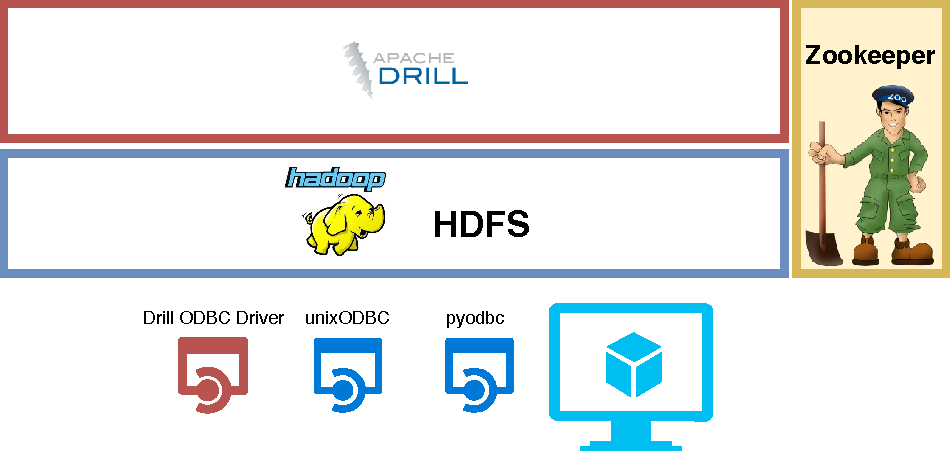
\includegraphics[width=\textwidth]{tech_stack}
				\caption{Technology stack}
			\end{figure}
		\clearpage
		\section{SIILCK}
		\label{sec:siilck}
		\subsection{Naming conventions}
		The overall design of SIILCK is object oriented, with a object named  \textbf{society} as the the overarching authority. The society holds the \textbf{knowledge} and all \textbf{candidates}, and the candidates hold the \textbf{solutions}. The top candidates carrying the best solutions are called \textbf{academics} and get added to a separate population called the \textbf{academia}, where they get to alter the collective knowledge, thus aiding in the generation of future candidates. When using SIILCK, one execution of the algorithm from start to end is called a \textbf{optimization process}, or simply a \textbf{process}. When a candidate applies its solution to a problem to test efficiency it is doing a \textbf{job}. A job can be a single task, a number of steps - or as in this thesis, a batch of queries. Once all candidates have performed jobs, academics are chosen and knowledge is altered that means one \textbf{generation} has passed, also called one \textbf{SIILCK cycle}. A SIILCK process runs until the collective knowledge has converged, and the best candidate from the latest generation is chosen, called the \textbf{converged candidate}. SIILCK then considers the solution object of the converged candidate to be the optimal for the respective problem. 
		\begin{figure}[H]
			\centering
			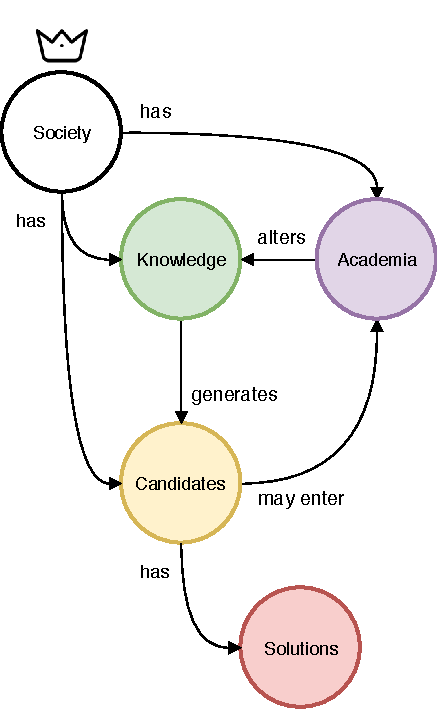
\includegraphics[width=200pt]{OOP}
			\caption{Hierarchy of objects}
		\end{figure}
		\subsection{Society}
		\label{sec:society}
		When initializing a optimization process the first crucial thing to get created is the society. The society extracts all of the information contained within the configuration file, to construct itself, the knowledge object, a default candidate and an initial population of candidates.
		\paragraph{Knowledge}
		The first thing the society needs to do, apart from declaring various variables to itself, is generating a knowledge object. Without the knowledge the society can't initialize any candidates, as they are dependent on the knowledge to define probability vectors for what options each parameter should initialize to within the solutions. The global genetic material that defines candidate creation within SIILCK is stored in the collective knowledge, or rather \textbf{is the collective knowledge}. The knowledge is further explained in the \hyperref[knowledge]{next subsection.} 
		\paragraph{Default candidate}
		To define goals for the fitness function a candidate is created, with all default values. This candidate also comes into play at the end of a optimization process, to verify that the converged candidate solution is effective. In the beginning, the default candidate simply performs a job the same way as all future candidates will, and metrics for mean, maximum and minimum TTE is stored within. The goal is then set at 50\% reduction from the default candidates min time, giving a somewhat unrealistic goal to ensure that we strive towards the most cost effective solution. In the end we run a gauntlet of jobs between the default candidate solution and the converged candidate solution, called the \textbf{solution assurance stage}, where we measure the averages - to ensure that there's no uncontrolled variance that led to the result. In SIILCK generally though, the fitness function can be anything the developer wants it to be.
		\pagebreak
		\paragraph{Population}
		Based on a parameter from the configuration file, the society generates an entire generation of \textit{n} candidates carrying solutions to the respective problem. For each generation the society measures the fitness of all candidates and removes the weakest ones. Then the strongest / fittest ones get added to the academia, which is a set of candidates we call the \textbf{academics}. The academics are the ones that refine the knowledge, incrementally adapting it and reinforcing good solutions. After the knowledge has been altered by the newly added academics (and potentially academics from earlier generations), new candidates get added to the population to replace the ones that got removed. The configuration file can drastically alter the way the population behaves, by changing values for operations that are done on each generation:
		\begin{itemize}
			\item The size of the population
			\item The size of the academia
			\item The number of candidate removals / replacements each generation
			\item The number of academics to add to the academia each generation
			   \begin{itemize}
				\item To keep the knowledge alterations based on fresh new solutions, we want to retire older academics, restricting Academia to a predefined amount of academics. This is generally a lower number than the population itself, but there are no restrictions. Retiring academics help convergence, since all academics then eventually will think alike the higher the generations. If there were no retirees there would be a lot of old academics altering the collective knowledge at a later stage, even though their solutions might no longer hold merit.
				\end{itemize}
		\end{itemize}
		\clearpage
		\subsection{Knowledge}
		\label{knowledge}
		The knowledge is the heart of SIILCK. It provides a centralized body of collective knowledge that helps construct solutions based on historic data, and incrementally adapts as new academics are being added. While SIILCK can be considered a machine learning technique, the knowledge has a truly finite usage within each process, as it is meant to reach a state of convergence. More classical incremental learning schemes are continuously adapting, attempting to for instance predict the stock market. In our case however we simply want to reach one final solution and then end the process. For each optimization process the knowledge starts out fresh, with a uniformly distributed probability vector, ensuring that changes in i.e cluster topology or data skewness will be taken into consideration when optimizing. Thus it can be valuable to execute one full optimization process each time a big data environment changes, or new data sources get added. If the knowledge were to store historic data, then certain probability vectors would be skewed in favor of previously strong solutions, that may not be beneficial for current or future processes. The knowledge object works by mirroring the solutions as a probability vector, thus allowing a solution to be any kind of complex value, as long as it in a list structure. For each parameter in the solution, there is a list of potential options. Those options can be anything from numbers to complex objects. For each parameter in the knowledge, there is a probability vector representing the chance to choose any of the options in the solution parameter when generating a candidate.
		\begin{figure}[H]
			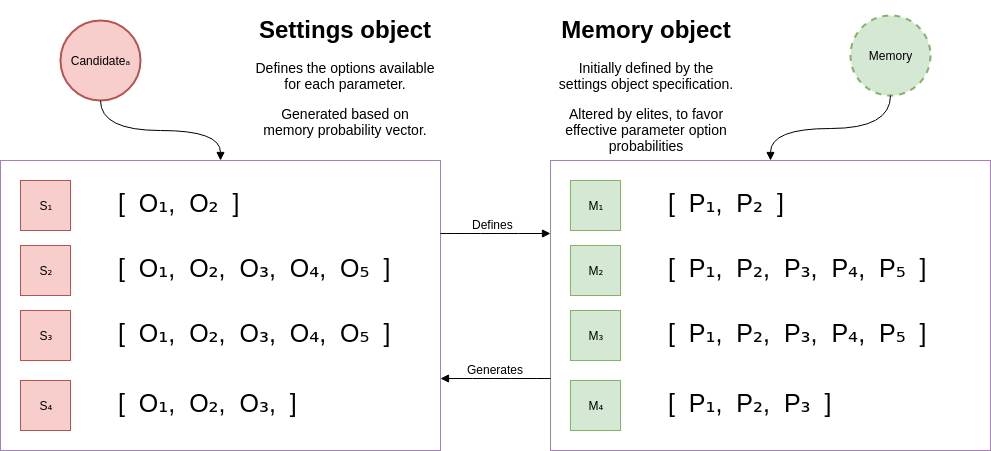
\includegraphics[width=\textwidth]{memory_candidate}
			\caption{The reliance between a candidates' solution object, and the collective knowledge.}
		\end{figure}
		\clearpage
		\paragraph{Probability vector algorithm}
		\begin{wrapfigure}{r}{5.5cm}
			\caption{How the knowledge gets altered by the academics}
			\label{fig:memory_insight}
			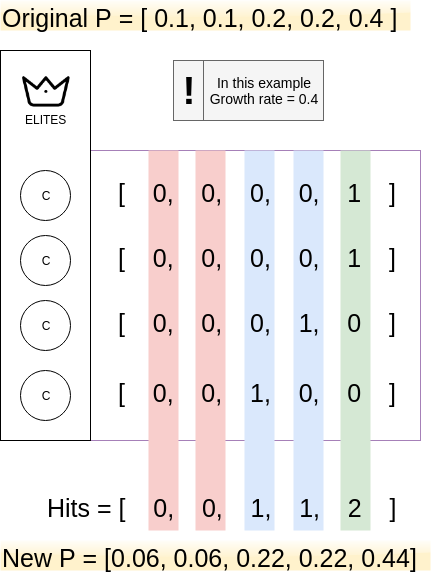
\includegraphics[width=5.5cm]{memory_insight}
		\end{wrapfigure} 
		When altering the knowledge, we iterate over each academic in the academia, and view their solution parameters. Each option for a given parameter in the academic is represented as a list, containing any type of data. The list can be as short or as long as the user likes - it will automatically get a uniform probability distribution in the knowledge and be eligible for optimization. For each parameter the academics solution object contains, there is a mirrored probability vector in knowledge. When the alterations take place, we check the academic parameter value and locate it in the list of options, and then return a binary list of hits. For instance if the parameter is boolean the logic would look like this:
		\begin{enumerate}
			\item Parameter value is \textbf{True}
			\item Parameter options are \textbf{[True,False]}
			\item Binary representation will be \textbf{[1,0]}
		\end{enumerate}
		Once this binary option conversion is done for all candidates, we sum up the hits of each option and get a single list for all accumulated hits, as seen in figure \ref{fig:memory_insight}. Finally we can apply the mathematical formula to alter the probability vector, using the accumulated hits list - as shown in equation \ref{math:probability_vector}.\\

		\begin{equation}\label{math:probability_vector}
		P_{i,j}(t) = P_{i,j}(t)+\lambda\left(\frac{\mu_{i,j(t)}}{|\mu|}-P_{i,j}(t)\right)
		\end{equation}
		{\centering
		\begin{math}
		P = probability, i = parameter, j = option, \mu = academic, t = time
		\end{math}\\
		}
		\paragraph{Reaching convergence}
		After each knowledge alteration the knowledge object checks itself, and each parameter within the solution object it holds. It then counts each parameter, and whether it has passed the convergence threshold. Once all parameters has passed the threshold convergence is reached.
		
		\paragraph{Academic consensus and critical convergence}
		In the beginning of a optimization process it is typical that all the academics that are added to the academia contain mostly the same options for essential parameters. This means that we have \textbf{academic consensus} on what parameters produce the best results, which leads to a steady increase in those option probabilities for their respective parameters - meaning a steady increase in overall convergence value. Once all those parameters have reached convergence (meaning that they have passed the convergence threshold), there may be more parameters left to converge, where the academics that get added don't share the same options. This means that we have lost academic consensus, and is also noted here as having reached \textbf{critical convergence}. Once the point of critical convergence is reached and academic consensus is lost, the remaining generations until full convergence are spent to converge arbitrary parameters, which may be a waste of time and resources. This is the reason for implementing accelerated convergence.
				
		\paragraph{Accelerated convergence}
		\label{sec:aggres}
		Once the total convergence value has reached 90\% of the convergence threshold, the knowledge enters a state of accelerated convergence. In this state the learning rate of the SIILCK increases by 0.2. This is due to parameter agnosticism in many problems, and especially in less complex problems or environments. This is further detailed in the discussion section, \hyperref[sec:param_agno]{parameter agnostic queries}.
		
		\subsection{Extended knowledge function - progress estimation}
		The knowledge object is also responsible for a novel approach to estimating the progress of a process. The single biggest drawback of using evolutionary algorithm techniques for complex problems is execution time, and especially as it's commonly impossible to predict. Still we are able to create two individual progress bars, to give users some idea of the time optimization should take.
		\linebreak
		\scriptsize
		\begin{verbatim}
		###############################
		########## Optimizing #########
		###############################
		
		
		|###########                                     |29.09 % of critical parameters converged
		
		|###################################             |74.90 % total convergence
		
		
		############ Testing generation 54 ############
		Accelerated convergency active
		Running Candidate 50.0
		Running Candidate 51.1
		Running Candidate 52.1
		Running Candidate 52.4
		Running Candidate 53.3
		Running Candidate 54.0
		Running Candidate 54.1
		Running Candidate 54.2
		Running Candidate 54.3
		Running Candidate 54.4

		\end{verbatim}
		\normalsize
		\pagebreak
		The first bar estimates when critical parameters are converged. This is done by tracking convergence values over time, and using a linear regression model to predict when the convergence threshold should hit. The linear regression model fails at one point, because the prediction starts to inverse - i.e it predicts that total convergence value should pass convergence threshold on generation \#60, while we're already at generation \#65. This then indicates strongly that academic consensus is missing, and the remaining values put forth begins to flatline, meaning only arbitrary parameters remain to be settled, meaning the system is estimated to have reached critical convergence. The second bar represents total convergence and is a simple and accurate function of current convergence * 100 - considering how current convergence is a number between 0-1.
		\begin{algorithm}
			\caption{Critical convergence estimation - pseudo code}\label{algo:critical_convergence}
			\scriptsize
			\begin{verbatim}
			
			# Estimate when convergence of critical parameters are done
			cl = list of all convergence values for generations passed
			il = list of cl indexes
			diff = list of all convergence differences for generations passed
			model = linear regression model
			fit model(cl,il)
			convergence = model.predict(#CONVERGENCE_THRESHOLD)
			diff.append(convergence - il[-1])
			
			target = max(diff)
			percentage = ((diff*(-1) + target) / target) * 100
			
			# Construct progress bar based on percentage
			
			USER DEFINED CONSTANTS:
			CONVERGENCE_THRESHOLD: Threshold for when a parameter is considered to be converged
			
			\end{verbatim}
		\end{algorithm}
		\clearpage
		Algorithm \ref{algo:critical_convergence} has been tested thoroughly and proven to be an effective estimation for critical convergence, with two such tests graph displayed in graph \ref{fig:estimation1} and \ref{fig:estimation2}. Further details on academic consensus, critical vs arbitrary parameters and parameter agnostic queries can be read in the discussion chapter, \hyperref[sec:param_agno]{Examples of agnosticism from stable cluster}
		\begin{figure}[H]
			\centering
			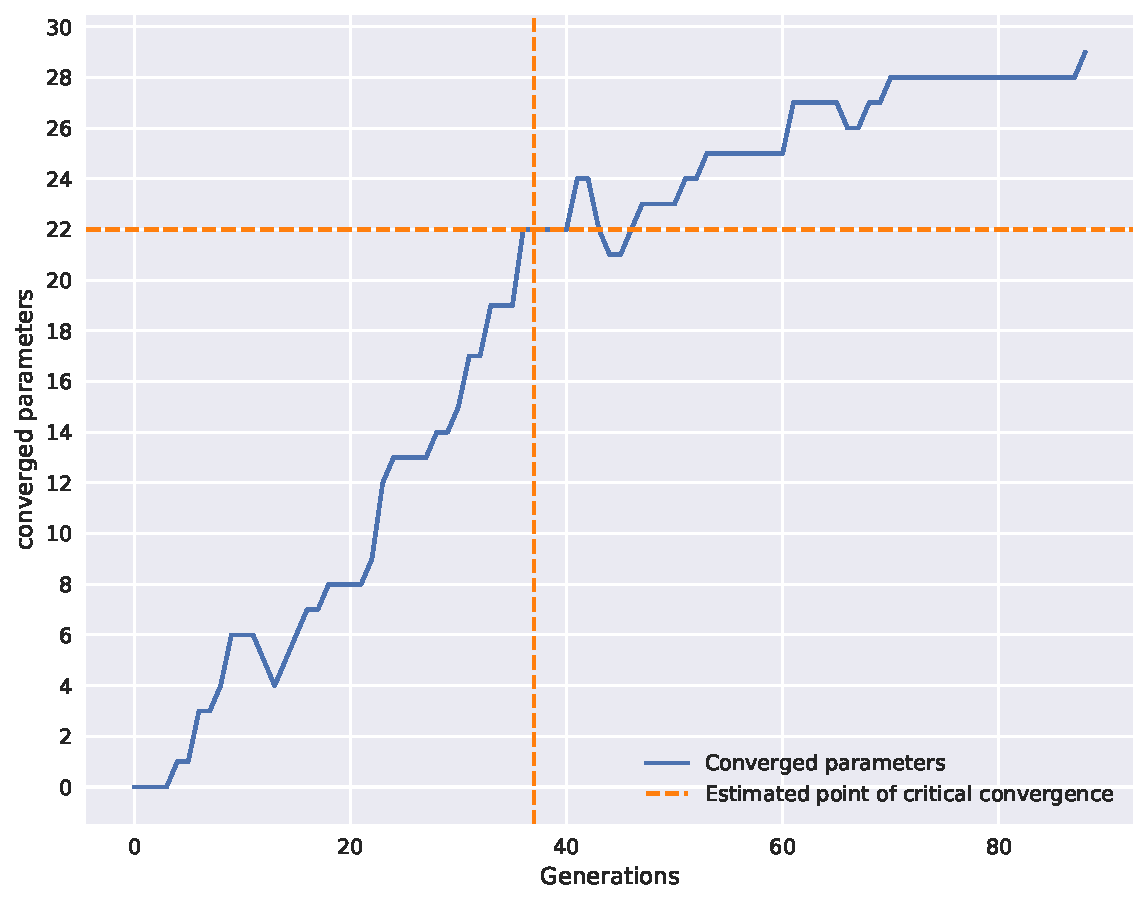
\includegraphics[width=260pt]{est11}
			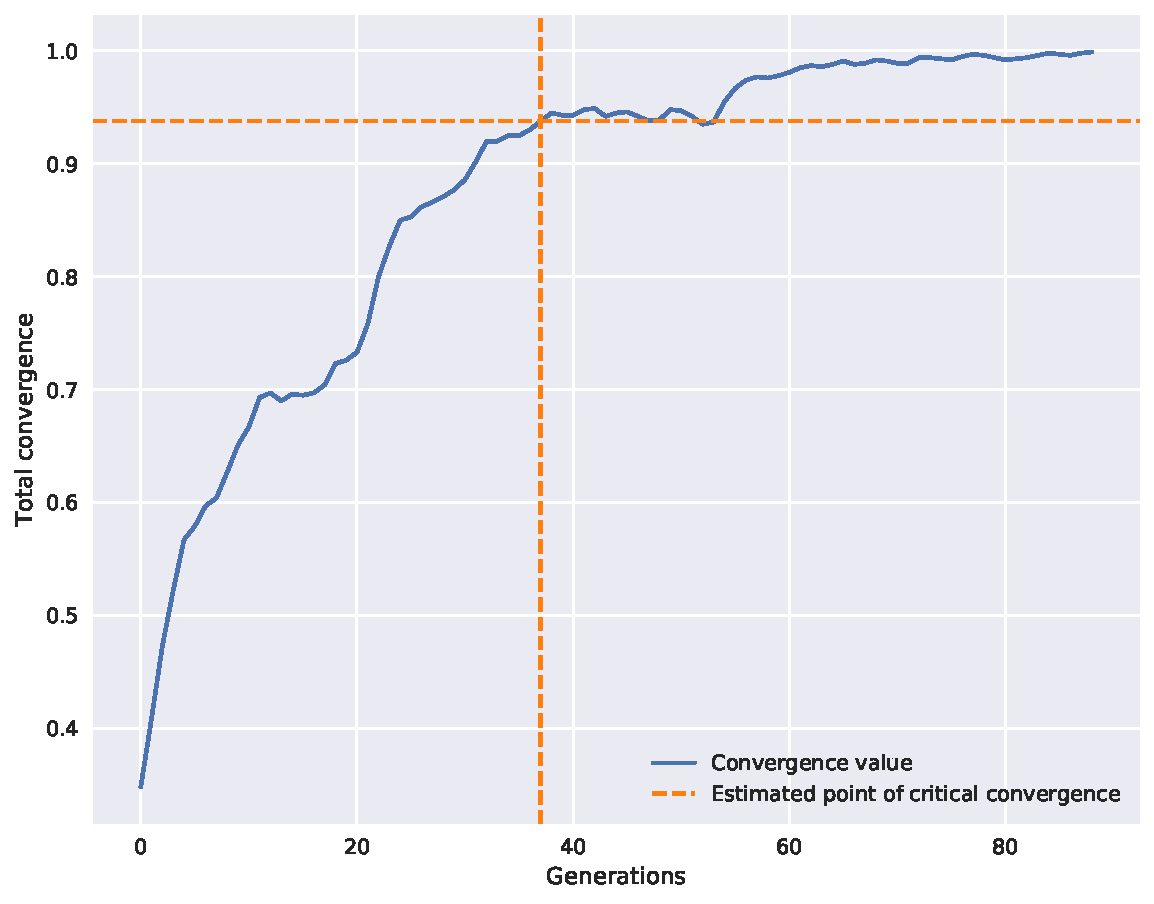
\includegraphics[width=260pt]{est12}
			\caption{Data from experiment N3, showing when the model estimated that the point of critical convergence was hit. The first graph shows the amount of parameters converged, and the second graph shows the total convergence value - for the same job. Estimated point of critical convergence can be observed as the point in time where total convergence value first starts to flatline. Critical convergence was achieved after 22 parameters was converged, indicating that the remaining 7 parameters are arbitrary for current workload in current environment.}
			\label{fig:estimation1}
		\end{figure}
		\begin{figure}[H]
			\centering
			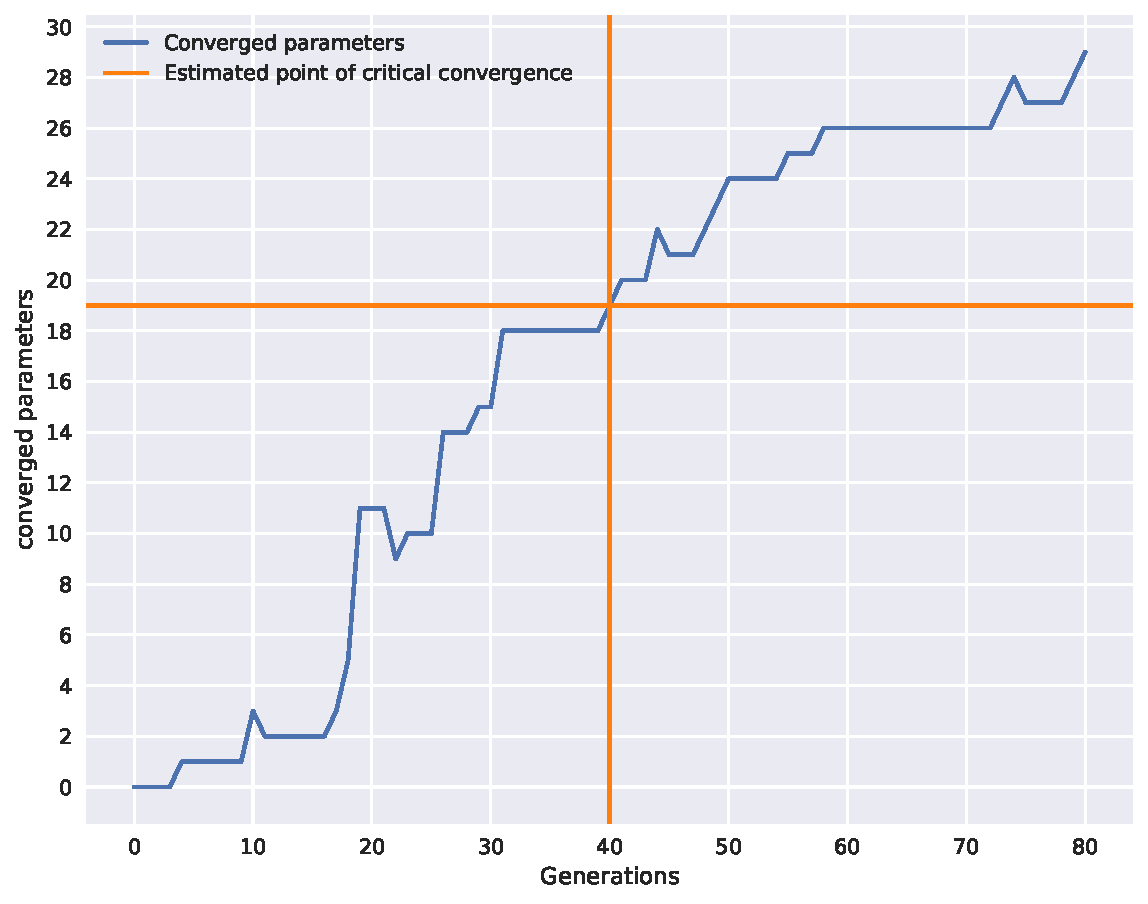
\includegraphics[width=260pt]{est21}
			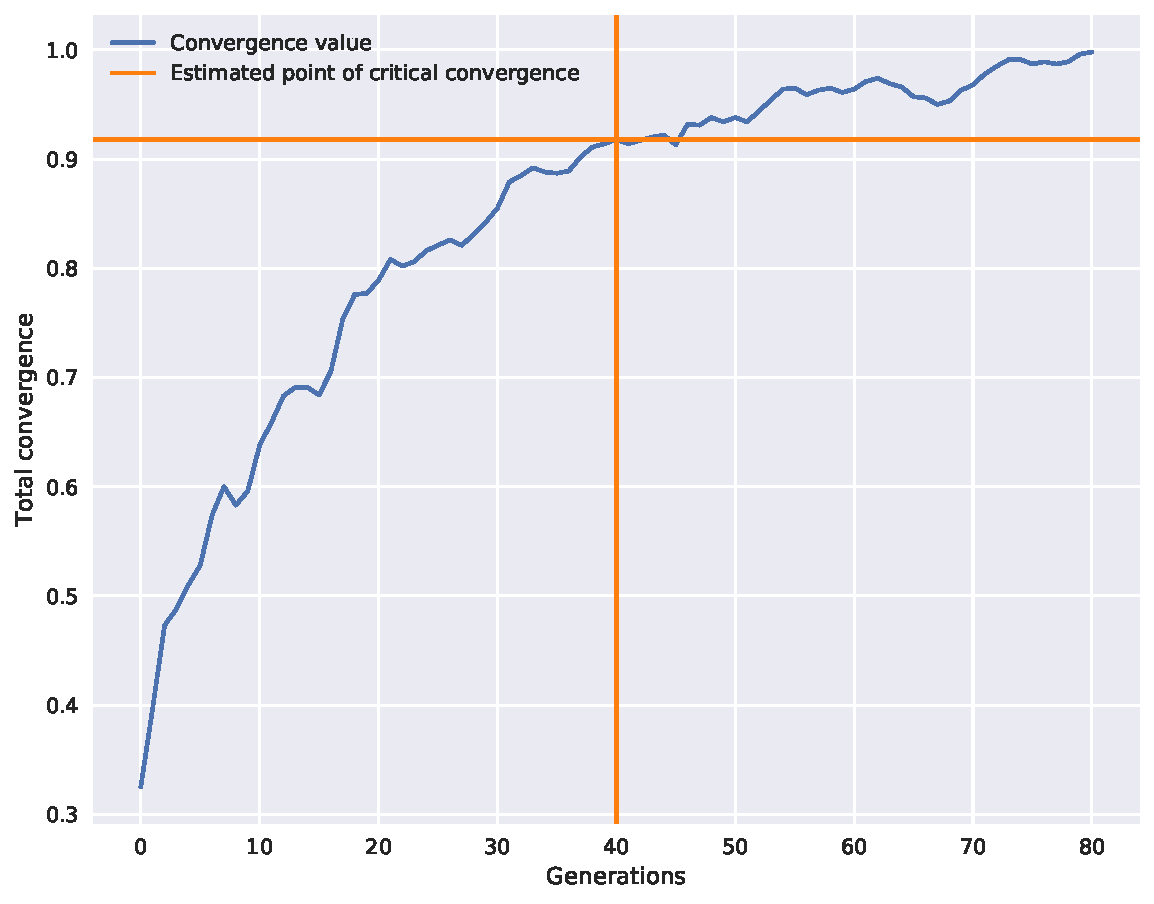
\includegraphics[width=260pt]{est22}
			\caption{Data from experiment E5 , showing when the model estimated that the point of critical convergence was hit. The first graph shows the amount of parameters converged, and the second graph shows the total convergence value - for the same job. Estimated point of critical convergence can also here be observed as the point in time where total convergence value first starts to flatline. Critical convergence was achieved after 19 parameters was converged, indicating that the remaining 10 parameters are arbitrary for current workload in current environment.}
			\label{fig:estimation2}
		\end{figure}
		More information about how many parameters that are critical, and how many that are arbitrary is detailed in the results chapter, \hyperref[sec:aggres]{aggregated results}.
		\clearpage
		\subsection{Candidate}
		Candidates don't hold much information on their own, as most of it is stored in a solution object, which the candidate holds on to. However the candidate has some crucial functions, like how to perform jobs (in this case how to perform queries) with their solution object, how to mutate and how to measure self performance.
		\paragraph{Jobs}
		To get data on whether or not a particular set of parameter options will be an effective solution in the current environment, we need to run some tests - here simply defined as jobs. To complete a job in the tailored application for drill the candidate is dependent on a data source, and information on how many queries to do, in order to measure the TTE. In a cluster where resources are shared among many users, or multiple queries are ran concurrently on the same quorum, the optimal solution need to take this into consideration. Therefore jobs are done in two stages, one for concurrency testing, and another for sequential testing. Both the data source and the number of queries to complete are defined by the configuration file. The data source defined here is a ODBC DSN, but for future work this can be easily altered to point to a JDBC DSN or other similar sources. The number of queries defined by the configuration file is actually doubled in runtime, as it defines both the amount of concurrent queries in addition to the amount of sequential queries. This means that defining this parameter to the absolute minimum of 1 query, results in two queries - one in the concurrent stage and one in the sequential stage. Performing only a single query would leave too much up to circumstance, in regards to the available resources in the cluster and random error, thus a minimum of two queries is needed to measure performance - although any number higher than that is advised. Further technical details on how the jobs are performed can be read in the \hyperref[sec:jobs]{testing section}
		\pagebreak
		\subsection{Mutation}
		To mitigate the issue of premature convergence a mutation function is in place, to mutate new candidates at a set probability defined by the configuration file. After a candidate is created, it may be chosen for mutation. The value that defines the probability for a candidate to be chosen also decides the probability for individual parameters to mutate within the candidates solution object. There is also a resistance value in place, to avoid too heavy mutations, potentially resulting in a useless candidate at later stages, which simply increases the time cost of the algorithm. The resistance value starts at 0, and increases via the resistance growth value set in the configuration file. Each time a parameter is mutated within a candidate, the candidate becomes more genetically resistant. It works by linearly reducing the mutation chance for individually chosen candidates. By default this reduction is 1\% per mutation. Increasing the resistance growth would result in more stable candidates, more purely defined by knowledge, but gives less variations - so this needs to be balanced. 
		\begin{figure}[H]
			\centering
			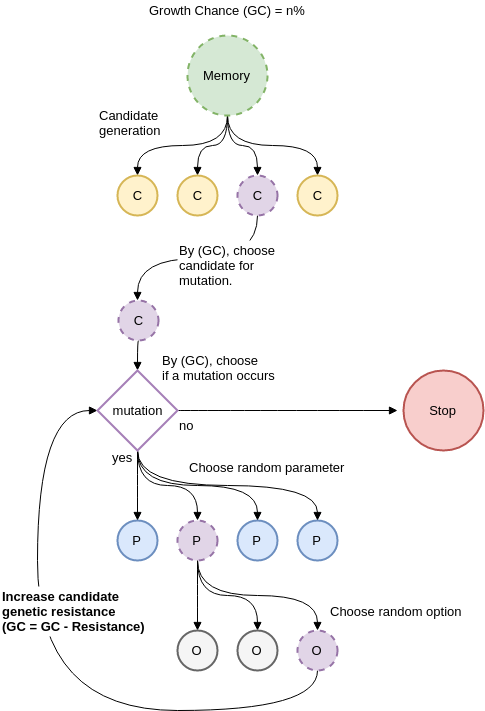
\includegraphics[width=250pt]{Mutation}
			\caption{Mutation function flowchart}
			\label{fig:mutation}
		\end{figure}
		The mutation is entirely isolated from the knowledge, and thus chooses a new option for the parameter randomly, within a candidate. If a mutation is specifically advantageous in the given environment the candidate will go on to become an academic, thus altering the knowledge with its newfound solution.
		\subsubsection{PBIL Mutation vs SIILCK Mutation}
		The original implementation of the PBIL mutation function seen in algorithm \ref{algo:pbil_mutation1} focused on mutation of the collective probability vector. The SIILCK approach seen in algorithm \ref{algo:pbil_mutation2} mutates individual candidates - hoping to produce a diverse set of academics. For the two algorithms \ref{algo:pbil_mutation1} and \ref{algo:pbil_mutation2}, mathematical annotations can be seen in annotation table \ref{table:annotations}. Furthermore the mathematical formula showing the probability for \textit{$\eta$} mutations in each candidate is shown in equation \ref{math:mutation_chance}.
		\begin{algorithm}
			\caption{Original PBIL mutation \cite{pbil}, with annotations changed to be consistent with thesis annotations. In PBIL the collective probability vector is directly mutated.}\label{algo:pbil_mutation1}
			\scriptsize
			\begin{algorithmic}
				
				\FOR{$length(\beta_{i})$}
					\IF{$rand(0,1) > P_{mut}$}
						\STATE $P_{i,j} = P_{i,j} * (1.0 - M) + rand(0,1) * M$
					\ENDIF
				\ENDFOR
			\end{algorithmic}
		\end{algorithm}
		\begin{algorithm}
		\caption{SIILCK mutation. In SIILCK the candidate solution is mutated.}\label{algo:pbil_mutation2}
		\scriptsize
			\begin{algorithmic}
			\REQUIRE C = new candidates in population
			\ENSURE $\varepsilon_{growth} = x \in (0 \leq x \leq 1) $
			\FOR{c in C}
			\IF{$rand(0,1) < P_{mut}$}
				\STATE $\varepsilon = 0$
				\WHILE{$ rand(0,1) < P_{mut} - \varepsilon $}
					\STATE $i_{n} = rand(0, length(c_{i})-1)$
					\STATE $c_{i_{n},j}  = rand(0,length(c_{i_{n},j})$
					\STATE $\varepsilon = \varepsilon + \varepsilon_{growth} / 10$
				\ENDWHILE
			\ENDIF
			\ENDFOR
			
			\end{algorithmic}
		\end{algorithm}
	
			\begin{equation}\label{math:mutation_chance}
			P_{mut}(\eta) = (P_{mut}-0 \varepsilon) * (P_{mut}-1 \varepsilon) \ldots * (P_{mut}-(\eta-1) \varepsilon)
			\end{equation}
			{\centering
				\begin{math}
				P = probability, \eta = amount, mut = mutation, \varepsilon = resistance
				\end{math}\\
			}
		\pagebreak
		\subsection{Solution}
		The solution object is simply a collection of parameters with available options, in this case session settings for Apache Drill to apply before running queries. An innovation of SIILCK is the ability to easily implement complex options in parameters as opposed to the binary representation of genetic material that GA or PBIL uses. As such, each parameter, representing a setting, is gathered from the documentation from the Apache team, and experimented on to see which ones affect TTE. The full list of parameters can be viewed in \hyperref[system_params]{appendix A}. \\ \hyperref[table:added_params]{Table A.1} shows what parameters where used, that where able to be altered in session. \hyperref[table:removed_params]{Table A.2} shows what parameters had to be cut, due to them only being able to be changed out of session, or them causing segmentation faults. 
		\subsection{Configuration file}
			This thesis focuses on removing the barrier for adoption of big data frameworks. As such one might find it ironic that a configuration file is supplied, that severely impact the performance of the optimization algorithm. However it is expected that the supplied default values set for the algorithm is sufficiently effective for any environment where this is run. With the default values there is a fine balance between execution time of the algorithm, and the effectiveness of the converged candidate solution. In addition to this there are very simple guide lines provided, regarding how big the cluster is, how many cores each node has, and how much time to be spent for accuracy sake. All the parameters can be found in \hyperref[table:conf_params]{appendix B}.
			\clearpage
		\subsection{Algorithm overview}
			\paragraph{Flowchart}
			Figure \ref{fig:sys_overview} shows a simplistic flowchart for an entire process, from start to achieved convergence.
			\begin{figure}[H]
				\centering
				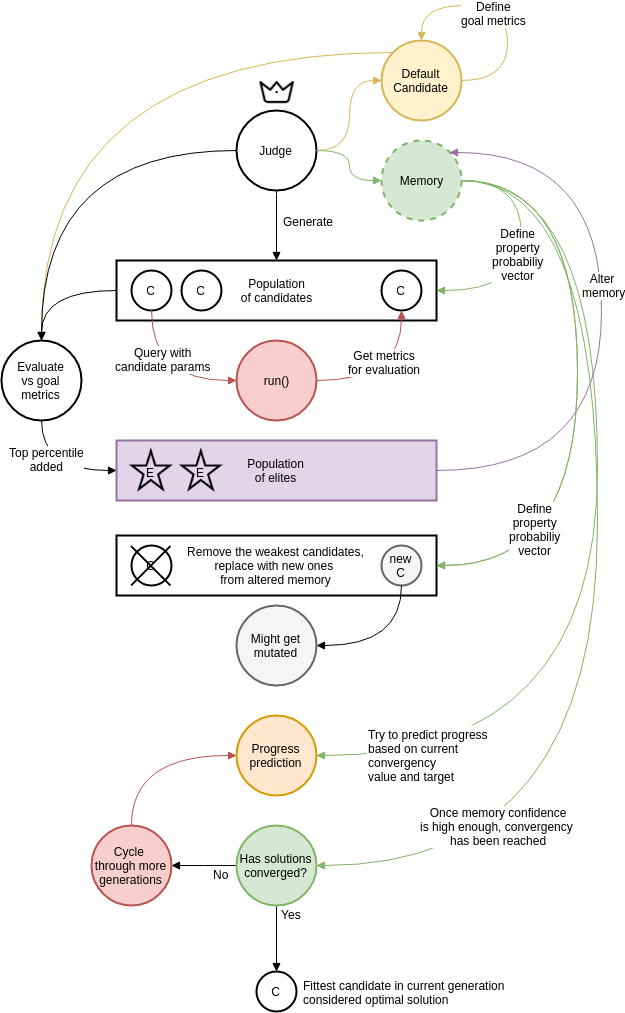
\includegraphics[width=330pt]{overview}
				\caption{SIILCK overview, tailored for Apache Drill optimization.}
				\label{fig:sys_overview}
			\end{figure}
			\clearpage
			
		\section{Experimental setup}
			\subsection{Dataset}
				The dataset used to test the algorithm on the clusters come from Yelp, specifically from their dataset challenge \cite{yelp}. The data was gathered as JSON files, containing reviews, stores, customer visits and the like.
			\subsection{Query}
				A query combining joins, grouping and sub queries was built to increase the complexity the Drill SQL EE had to handle. Further more the Drill specific notation KVGEN and FLATTEN was used for Key Value Generation after Flattening a complex json value to represent it as a table: \\
				\begin{flushleft}
				{\scriptsize 	
				SELECT Business, Days, Total\_Checkins \\
				FROM (SELECT Business, Days, SUM(tot1.Checkins.`value`) as Total\_Checkins\\
				FROM (SELECT tot.name as Business, tot.timvals.key as Days,\\ FLATTEN(KVGEN(tot.timvals.`value`)) as Checkins\\
				FROM (SELECT FLATTEN(KVGEN(tbl.`time`)) as timvals, business.name\\
				FROM (SELECT * FROM `/user/hadoop/drill/yelp\_data/checkin.json` LIMIT 1000) as tbl\\
				JOIN `/user/hadoop/drill/yelp\_data/business.json` as business\\
				ON business.business\_id=tbl.business\_id) as tot) as tot1\\
				GROUP BY Business,Days) WHERE Total\_Checkins$>$150 ORDER BY Business,Total\_Checkins\\
				}
				\end{flushleft}
			\clearpage
			\subsection{Job flowchart}
				\label{sec:jobs}
				Performing queries on the cluster programatically through python requires many layers of middleware. The Python language uses pyodbc, to speak to ODBC, that has defined a DSN on the Zookeeper Quorum, to access the Drillbits that reside on HDFS, as seen in figure \ref{fig:run_workflow}. Every time a query is run we measure the time it takes, and store it in a global list. This is important in regards to concurrency, as the threads themselves cannot return values to the main function, but rather append their values to a fixed index in the result list.
				\begin{figure}[H]
					\centering
					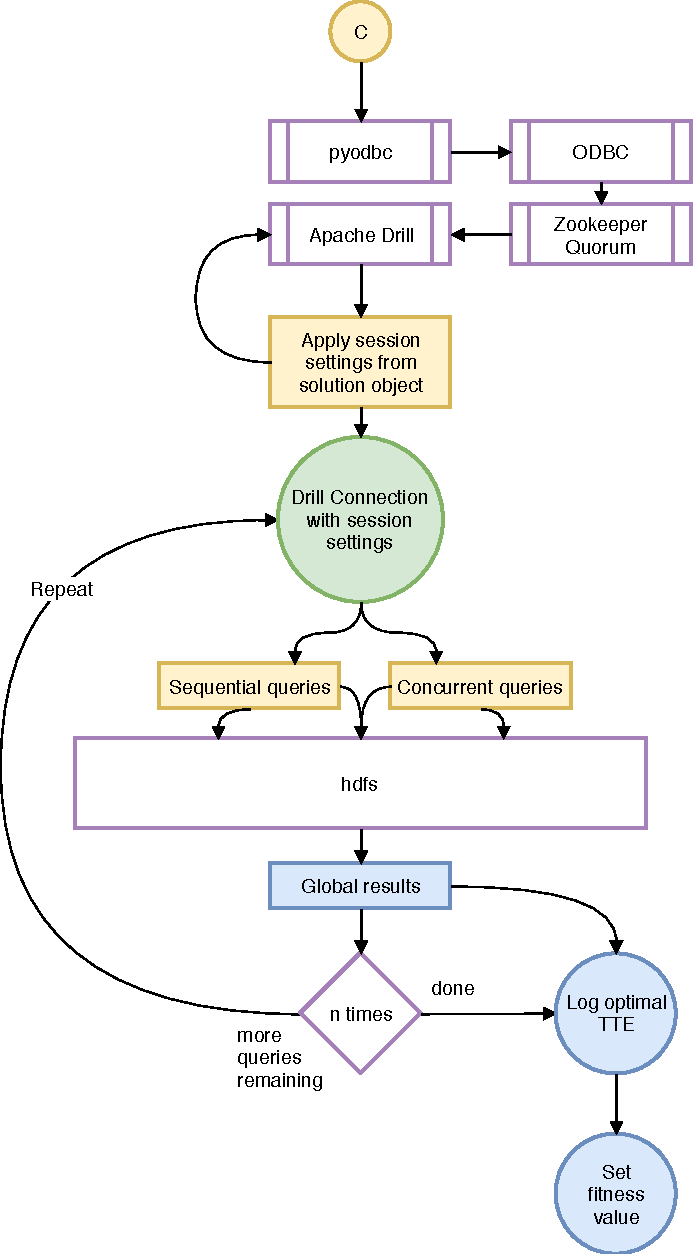
\includegraphics[width=240pt]{run_workflow}
					\caption{All the technological layers and steps that we pass during a single candidate job.}
					\label{fig:run_workflow}
				\end{figure}
			\clearpage
			\subsection{Data collection}
				When executing a job from a candidate we preferably do many queries before measuring fitness. The SQL syntax and the data is always the same between all candidates, job and queries. In addition to this we only take the optimal TTE into consideration when measuring a candidates effectiveness. This counts for all candidates generated from knowledge as well as the default candidate, as shown in figure \ref{fig:run_workflow}. This ensures they all compete on even ground, and no noise or variance effects the result. When performing a optimization, a user can either input a custom name for the process, or simply execute it without arguments, causing the name to be \textit{default}. After the scores are settled, all the collected data is stored in the logging folder under the chosen name, stored as a JSON file named as current timestamp. Data collected is:
				\begin{itemize}
					\item how many generations the optimization took
					\item average, mean and optimal query times for all academics
					\item average, mean and optimal query times for default candidate
					\item average, mean and optimal query times for default candidate and optimal solution during assurance jobs
					\item Cost saving for all candidate solutions vs default benchmark solution
					\item Total convergence values for all generations
				\end{itemize}
				All graphs presented in the results chapter \ref{chap:results} are generated based on this JSON file. In addition to the JSON file, a file named log.txt is generated for each successful optimization, containing the optimal solution parameters in relation to the default solution- looking like:
				\scriptsize
				\begin{verbatim}
					#### RUN: 2018.04.16.19.44.55
					Setting                                            Default value     Optimal value  Confidence
					----------------------------------------------  ----------------  ----------------  ------------
					planner.memory.enable_memory_estimation              0                 1            100.00%
					exec.queue.enable                                    0                 0            100.00%
					planner.broadcast_factor                             1                 0.75         100.00%
					planner.broadcast_threshold                          1e+07             5e+06        100.00%
					planner.slice_target                              1000              5000            100.00%
					planner.width.max_per_query                       1000               100            100.00%
					exec.min_hash_table_size                         65536             32768            100.00%
					exec.max_hash_table_size                             1.07374e+09       1.07374e+09  100.00%
					exec.queue.large                                    10                 2.5          100.00%
					exec.queue.small                                   100                50            99.98%
					exec.queue.threshold                                 3e+07             4.5e+07      100.00%
					exec.queue.timeout_millis                       300000            450000            100.00%
					planner.memory.max_query_memory_per_node             2.14748e+09       2.14748e+09  100.00%
					planner.width.max_per_node                          11                 9            100.00%
					planner.add_producer_consumer                        0                 0            100.00%
					planner.enable_hashjoin_swap                         1                 0            100.00%
					planner.enable_mergejoin                             1                 0            100.00%
					planner.filter.max_selectivity_estimate_factor       1                 1            100.00%
					planner.filter.min_selectivity_estimate_factor       0                 0.4          100.00%
					planner.join.hash_join_swap_margin_factor           10                12.5          100.00%
					planner.join.row_count_estimate_factor               1                 0.75         100.00%
					planner.memory.average_field_width                   8                14            100.00%
					planner.memory.hash_agg_table_factor                 1.1               1.5          100.00%
					planner.memory.hash_join_table_factor                1.1               1.1          100.00%
					planner.memory.non_blocking_operators_memory        64               128            100.00%
					planner.partitioner_sender_max_threads               8                 4            100.00%
					planner.nestedloopjoin_factor                      100               125            100.00%
					planner.producer_consumer_queue_size                10                50            97.58%
					store.text.estimated_row_size_bytes                100               400            99.99%
					store.json.all_text_mode                             0                 0            100%
					store.json.read_numbers_as_double                    0                 0            100%
				\end{verbatim}
				\normalsize
			\subsection{Solution assurance}
			As mentioned earlier we only use optimal TTE to measure default candidate and solutions, to reduce noise. However another layer of noise reduction was added at the end of the algorithm process, to ensure that no individual variance or noise caused the solution to be picked, even with purely optimal TTEs. This is named the solution assurance stage, running several jobs, 10 by default, where the converged candidate solution competes against the default candidate solution. Furthermore to make sure no cluster instability skews the assurance in any candidates favor, the default candidate and converged candidate take turns doing jobs - meaning the default solution is applied every nth job.
			\subsection{Adapting data collection}
			Because of the object oriented approach of this algorithm, where the society owns all the data, and gets passed along as an object for storing the data, it is really simple to adapt what to store. Every kind of metric belongs to the society, and the society is last object that we interact with before writing to disk. Therefore future work, or other use cases for SIILCK should have no problem with metric analysis, even on complex structures like nested objects or lists.
			
	\chapter{Results}
	\label{chap:results}
	\section{What we display}
	\paragraph{Graphs overview}
	Following the reasoning laid out in the \hyperref[chap:method]{method chapter}, we've ran several experiments. As the experiments were carried out, the data collected was slowly refined until we reached a final version where every source of noise was gone, and the graphical output to the user was meaningful and easy to read. Naturally then, all data showed in this chapter is collected from experiments performed on the \hyperref[table:cluster_stable]{stable cluster}. The main metric we measure to decide upon algorithm effectiveness is the \textit{Minimum query} value - which tests both the default candidate and the converged candidate under optimal conditions. Metrics for TTE, convergence and fitness for experiments are shown. In addition to this a graph for the solution assurance stage is included for each experiment, to clearly visualize the default candidate performance vs the converged candidate solution from SIILCK.
	\paragraph{Cost saving graphs}
	Data collection for the cost saving graphs, are gathered as the generations pass. It is based on each academic from its respective generation, vs the default candidates first job, which sets the benchmark goal. This first default job often turns out to be a high TTE outlier in Drill, which means the cost saving looks to be a lot higher than the solution assurance stage proves. This is further discussed in the discussion chapter, \hyperref[sec:cache]{drill cache}.
	\paragraph{Mean calculations for academic jobs}
	There are averages plotted in the academic job graphs, that are smoothed considerably for visualizing the results better. The averages are calculated by first collecting all academic jobs for a generation (by default 3), and averaging their results so we get a generation TTE. Then we add this generation TTE to a list, times the amount of academics we measured. Finally we perform Gaussian smoothing on the generated list twice. This makes the mean line smooth and easy to read. The functions can be viewed in appendix \ref{sec:plotting}, or in the GitLab repo: pydrill/plotting.py (functions \textit{smoothListGaussian} and \textit{create\_query\_mean})
	\clearpage
	\section{Run configurations}
	Configurations used were the same for all experiments, namely:
	\begin{verbatim}
	
		{
		
		"POPULATION_SIZE": 10,
		"GROWTH_FACTOR" : 0.4,
		"GROWTH_CHANCE" : 0.2,
		"RESISTANCE" : 0.1,
		
		"CONVERGENCE_THRESHOLD" : 0.95,
		"MAX_GENERATIONS" : 200,
		"CONCURRENT_RUNS" : 2,
		
		"REPLACEMENTS_EACH_RUN" : 5,
		"ELITES_EACH_RUN" : 3,
		"ELITE_CLUB_SIZE" : 7,
		
		"DATA_SOURCE" : "drill64",
		"NODES" : 4,
		"CORES" : 4,
		"NODE_LEAST_MEMORY" : 2147483648,
		
		"DISPLAY_OUTPUT" : false,
		"LOGGING_FOLDER" : "$HOME/runlogs/",
		"RUN_NAME" : "default"
		
		}
		
	\end{verbatim}
	Because of the very low memory specifications in the \hyperref[table:cluster_stable]{stable cluster}, we had to settle for a query amount value of 2, meaning 4 queries per candidate job. This is in actuality lower than advised for the algorithm to run effectively and produce certain solutions. Even so we could see an improvement in all experiments done during the solution assurance stage, proving that the algorithm performs well even under less than optimal settings, in low end environments. NB: The naming conventions of the configuration file follows the code, and not the abstract description of SIILCK, translations found in table \ref{table:code_names}. Further more GROWTH\_FACTOR is traditionally called learning rate, and GROWTH\_CHANCE describes mutation chance.
	\clearpage
	\section{Highlighted experiments}
	\subsection{Experiments done}
	There is data from eight experiments collected and shown in this thesis. They are called E1-E5 and N1-N3. The E simply represents the word experiment, and the N represents non-accelerated experiments.
	\label{sec:highlighted}
	\subsection{Which experiments we highlight}
	The experiments chosen for this section are simply the top 3, measured by cost saving. This means that there were no cherry picking for nice graphs or easily representable data. The top three experiments were:
	\begin{itemize}
		\item E1 at 1.99\% cost saving
		\item E3 at 1.74\% cost saving
		\item E5 at 1.64\% cost saving
	\end{itemize}
	\pagebreak
	\subsection{Experiment E1}
	\begin{verbatim}
	
	
	Convergence threshold reached at generation 66
	
	
	Results:
	Metric           Optimal solution    Default  Overhead saved
	-------------  ------------------  ---------  ----------------
	Optimal query             8.99453    9.17743  1.99%
 
		
	\end{verbatim}
	Experiment E1 achieved 1.99\% reduction in optimal query times, which is the highest cost saving in any of our recorded experiments, in 66 generations before converging. The convergence graph \ref{fig:final11} rises steadily meaning academic consensus was healthy for the process, never flatlining. This is also the reason for the early convergence at 66 generations. Figure \ref{fig:final13} shows the optimal query times for each academic gathered from each generation. It is strongly correlated with the cost saving graph \ref{fig:final12}, where we can see that both graphs appear chaotic for the first 100 academics recorded. These jumps in TTE is regarded as a random error, and it was due to a network backup snapshot done by Zookeeper - claiming many resources from the entire cluster. It is worth noting that the cost saving graph compares academic jobs to the default benchmarking job, which was clearly heavily affected by the snapshot, which is the reason for showing upwards of 16\% cost saving. As mentioned previously a faulty default benchmarking job ultimately does not interfere with calculating cost saving because of the solution assurance stage. Figure \ref{fig:final14} proves this, as it shows that the default candidate is around 0.2 seconds slower across all jobs counted which is just above 2\% as opposed to the 16\% from the cost saving graph. Naturally this also means that the solution assurance graph proves that the converged candidate solution repeatedly performs better in the 10 subsequent jobs performed during the solution assurance stage. A really interesting observation to make was that there clearly was academic consensus even though results varied wildly during the snapshot, meaning it didn't interfere with the fitness function. Once the snapshot was over TTE quickly falls to around 9 seconds and stays there, even through the solution assurance stage.
	\clearpage
	\begin{figure}[H]
		\centering
		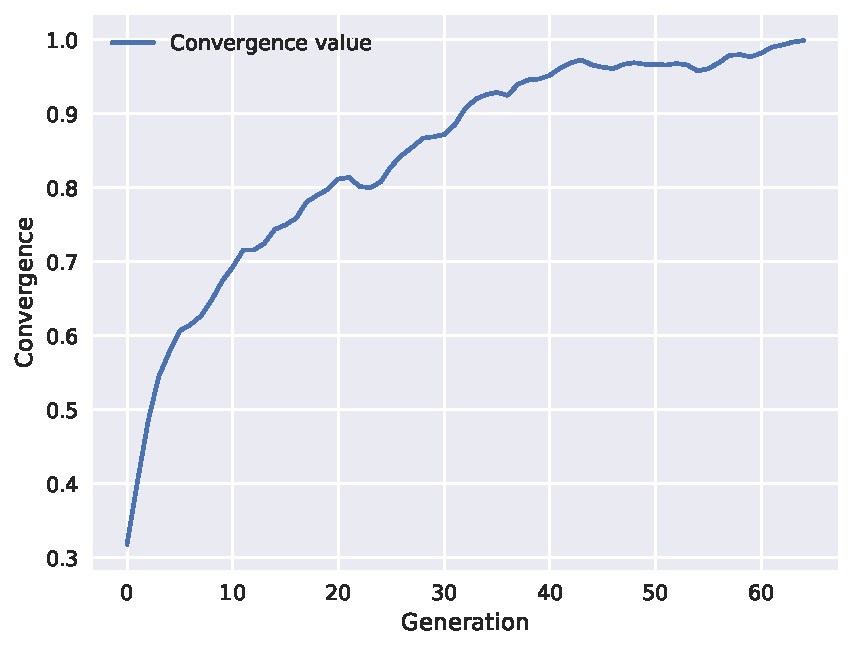
\includegraphics[width=300pt]{runlogs/final5/1}
		\caption{Experiment 1: Total probability convergence over generations}
		\label{fig:final11}
	\end{figure}
	\begin{figure}[H]
		\centering
		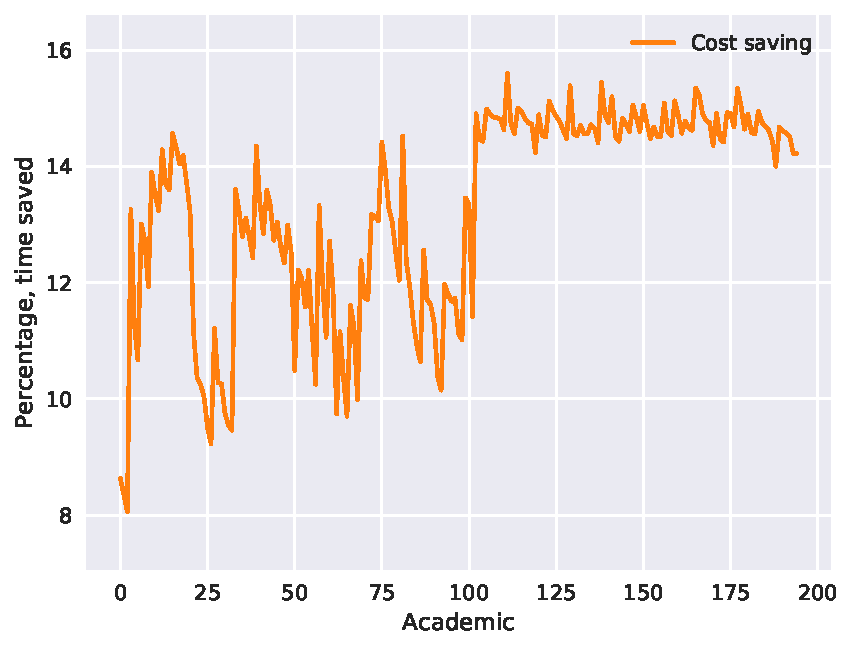
\includegraphics[width=300pt]{runlogs/final5/2}
		\caption{Experiment 1: Cost saving of optimal academic job vs default benchmark}
		\label{fig:final12}
	\end{figure}
	\begin{figure}[H]
		\centering
		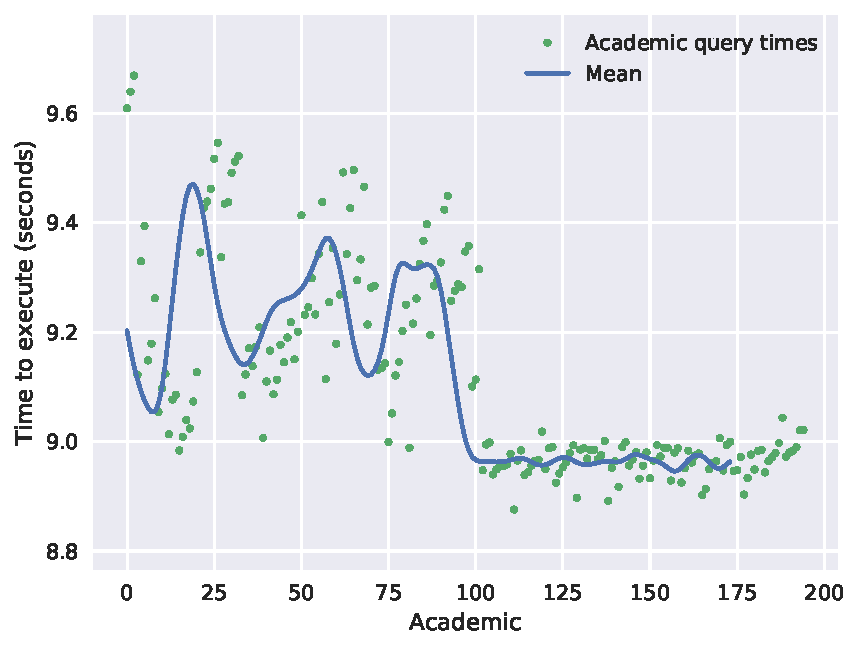
\includegraphics[width=300pt]{runlogs/final5/3}
		\caption{Experiment 1: Academic job graph, showing academics optimal TTE over generations}
		\label{fig:final13}
	\end{figure}
	\begin{figure}[H]
		\centering
		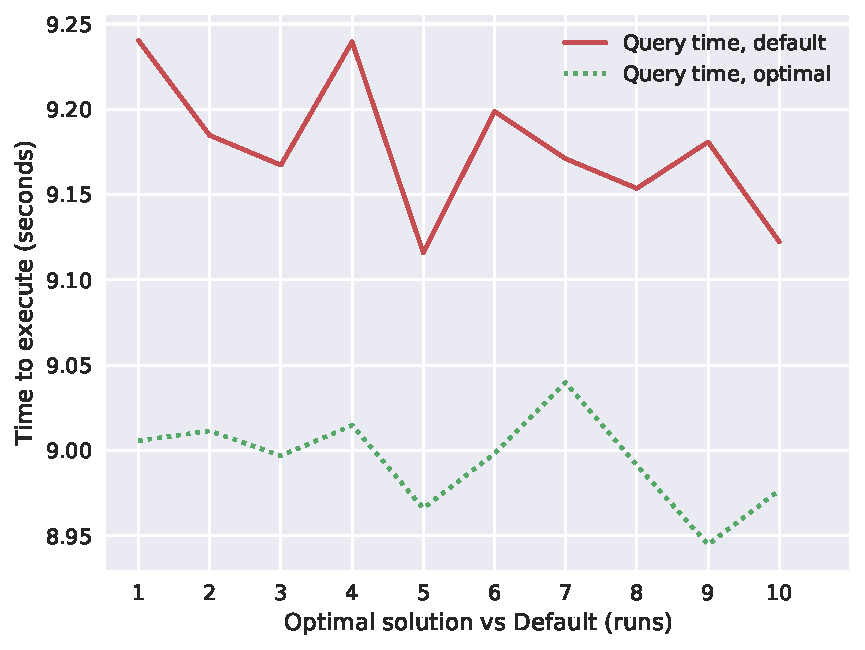
\includegraphics[width=300pt]{runlogs/final5/4}
		\caption{Experiment 1: Solution assurance stage, showing optimal solution vs default candidate}
		\label{fig:final14}
	\end{figure}
	\clearpage
	\subsection{Experiment E3}
	\begin{verbatim}
	
	
	Convergence threshold reached at generation 115
	
	
	Results:
	Metric           Optimal solution    Default  Overhead saved
	-------------  ------------------  ---------  ----------------
	Optimal query             9.00278    9.16258  1.74%

	
	\end{verbatim}
	Experiment E3 achieved 1.74\% reduction in optimal query times, in 115 generations before converging, being the highlighted experiment that took the longest to converge, whilst still utilizing accelerated convergence. This can be seen in the convergence value graph \ref{fig:final21}, where it dips at around generation 60. After dipping, and without academic consensus it takes a long while to reestablish convergency growth. The cost saving graph \ref{fig:final22} and the academic job graph \ref{fig:final23} both quickly stabilize and oscillate at around academic 50, meaning generation 17, so it was quick to reach a suitable solution. Viewing the solution assurance graph \ref{fig:final24} shows that the converged candidate solution repeatedly beats the default candidate.
	\clearpage
	\begin{figure}[H]
		\centering
		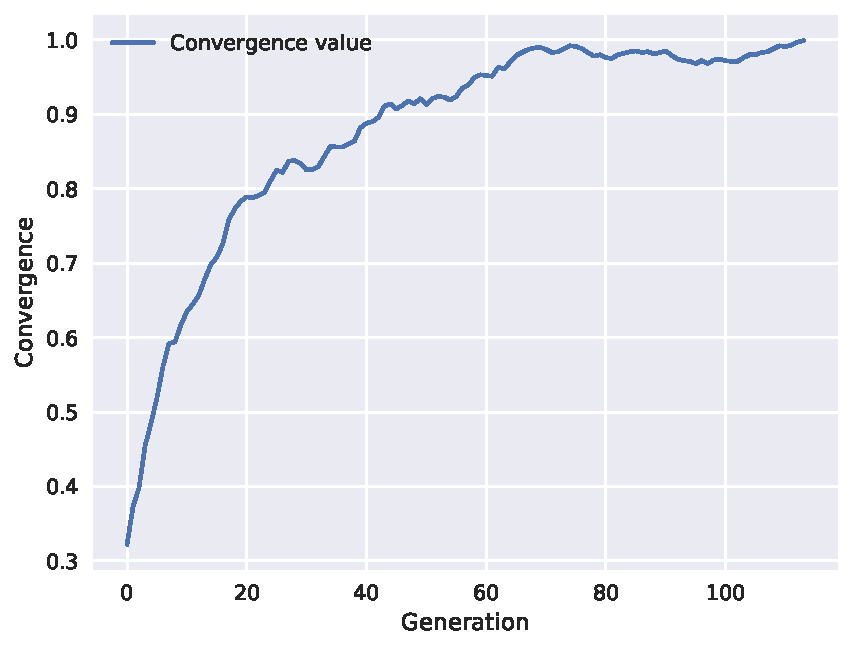
\includegraphics[width=300pt]{runlogs/final7/1}
		\caption{Experiment 2: Total probability convergence over generations}
		\label{fig:final21}
	\end{figure}
	\begin{figure}[H]
		\centering
		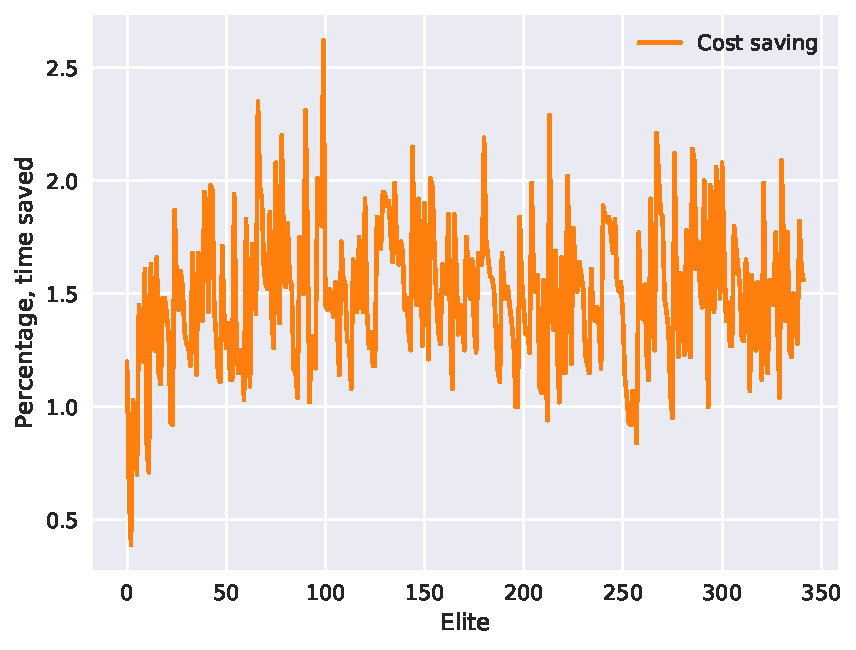
\includegraphics[width=300pt]{runlogs/final7/2}
		\caption{Experiment 2: Cost saving of optimal academic job vs default benchmark}
		\label{fig:final22}
	\end{figure}
	\begin{figure}[H]
		\centering
		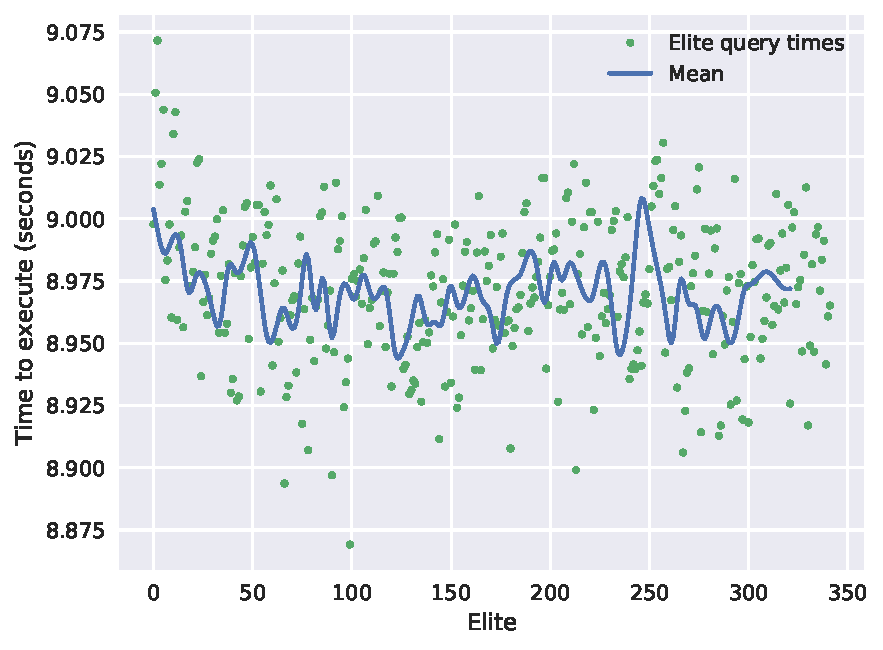
\includegraphics[width=300pt]{runlogs/final7/3}
		\caption{Experiment 2: Academic job graph, showing academics optimal TTE over generations}
		\label{fig:final23}
	\end{figure}
	\begin{figure}[H]
		\centering
		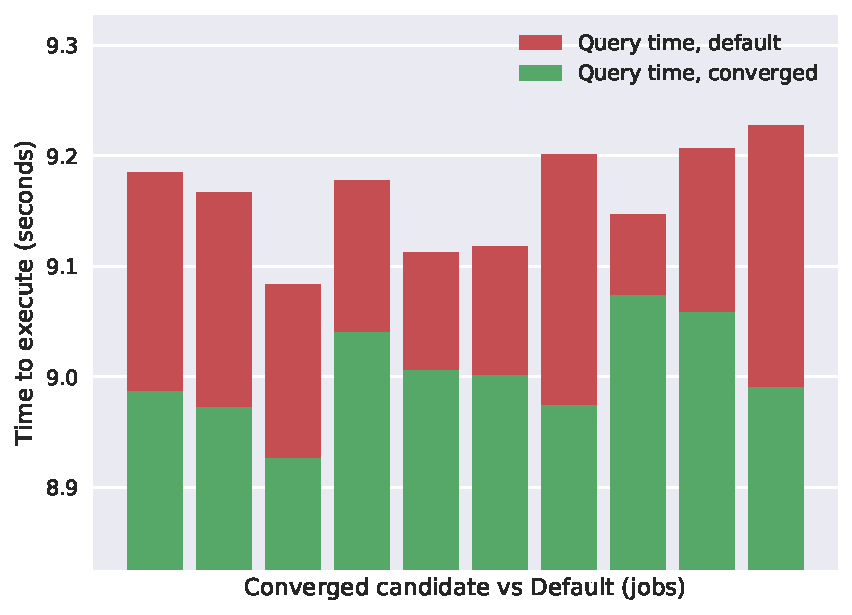
\includegraphics[width=300pt]{runlogs/final7/4}
		\caption{Experiment 2: Solution assurance stage, showing optimal solution vs default candidate}
		\label{fig:final24}
	\end{figure}
	\clearpage
	\subsection{Experiment E5}
	\begin{verbatim}
	
	
	Convergence threshold reached at generation 82
	
	
	Results:
	Metric           Optimal solution    Default  Overhead saved
	-------------  ------------------  ---------  ----------------
	Optimal query             9.01944    9.16986  1.64%

	
	\end{verbatim}
	Experiment E5 achieved 1.64\% reduction in optimal query times in 82 generations. As with experiment E1 the convergence graph \ref{fig:final31} never really flatlines, rather continuing on a upward trend until reaching total convergence. Very similarly to experiment E3 The cost saving graph \ref{fig:final32} and the academic job graph \ref{fig:final33} quickly finds a baseline to oscillate around, here being around 9 seconds. During the solution assurance stage shown in graph \ref{fig:final34} the converged candidate solution consistently beats the default candidate in every job counted.
	\clearpage 
	\begin{figure}[H]
		\centering
		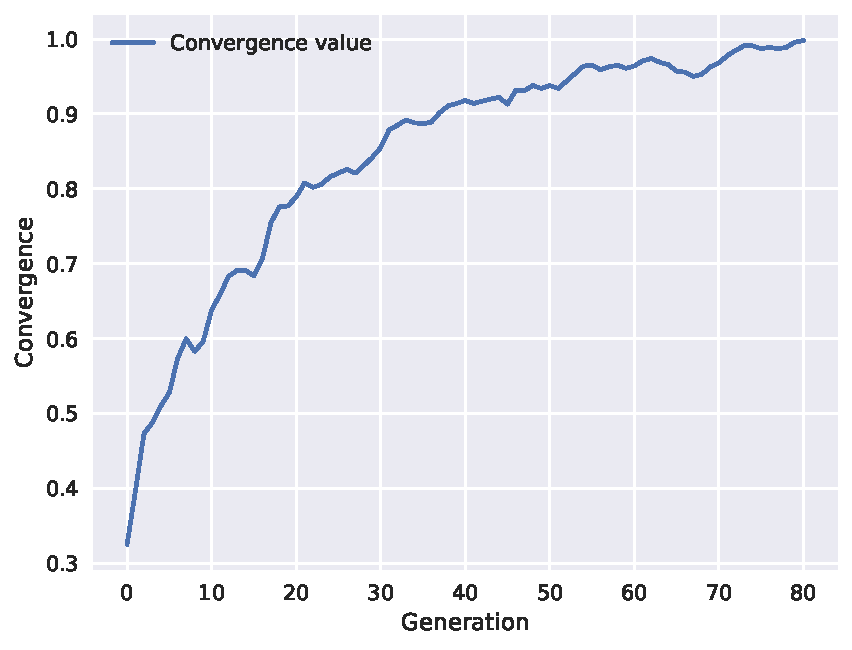
\includegraphics[width=300pt]{runlogs/final9/1}
		\caption{Experiment 3: Total probability convergence over generations}
		\label{fig:final31}
	\end{figure}
	\begin{figure}[H]
		\centering
		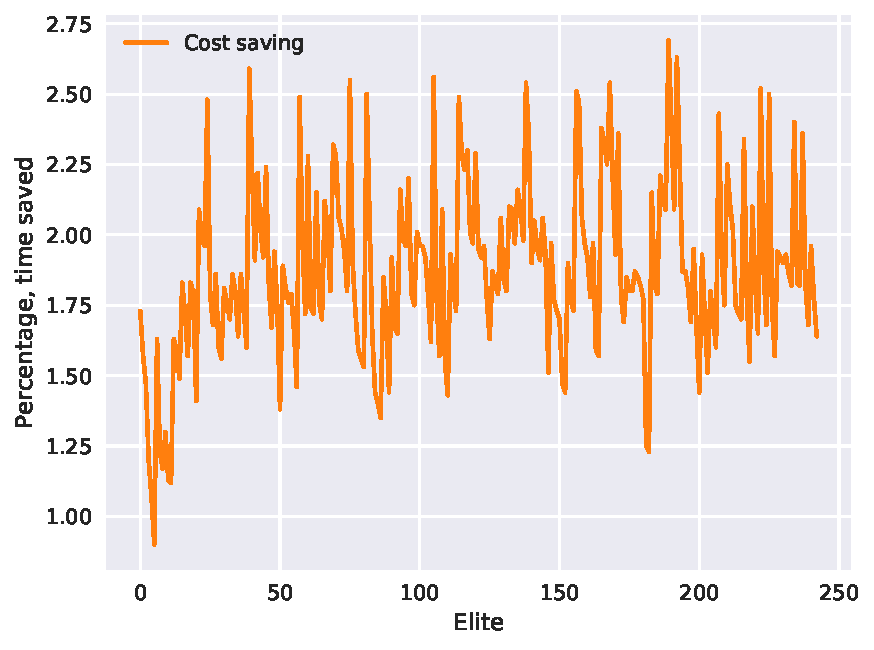
\includegraphics[width=300pt]{runlogs/final9/2}
		\caption{Experiment 3: Cost saving of optimal academic job vs default benchmark}
		\label{fig:final32}
	\end{figure}
	\begin{figure}[H]
		\centering
		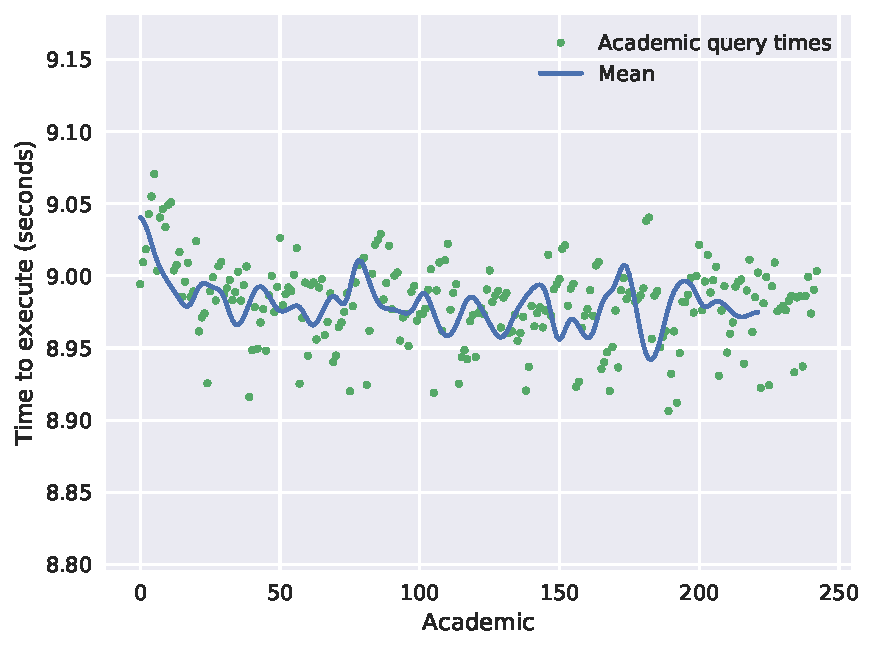
\includegraphics[width=300pt]{runlogs/final9/3}
		\caption{Experiment 3: Academic job graph, showing academics optimal TTE over generations}
		\label{fig:final33}
	\end{figure}
	\begin{figure}[H]
		\centering
		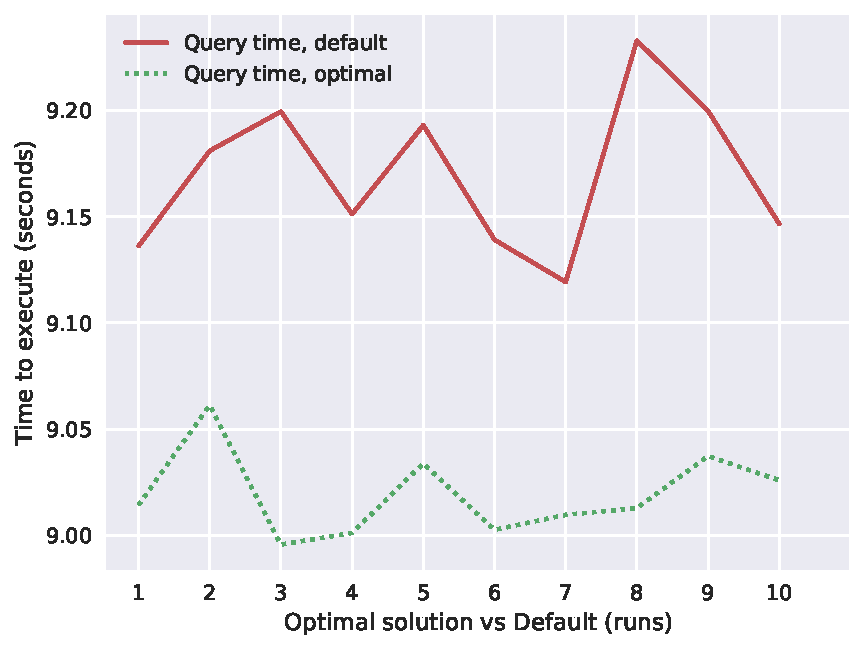
\includegraphics[width=300pt]{runlogs/final9/4}
		\caption{Experiment 3: Solution assurance stage, showing optimal solution vs default candidate}
		\label{fig:final34}
	\end{figure}
	\clearpage
	\section{Aggregated results}
	
	\subsection{Critical convergence and critical parameters}
	\paragraph{Critical convergence} The first thing to note is when critical convergence usually happens, and this can be observed in graph \ref{fig:criticalconv}. Drawing conclusions from table \ref{table:criticalconv} we can estimate based on the mean that it takes around 37 generations (37.375) for critical convergence, no matter how long total convergence takes. With a sample standard deviation of 3.35, we get a confidence level of 68,3\% for results within 36.1 - 38.6 and 90\% within 35.3 - 39.4.
	\begin{figure}[H]
		\centering
		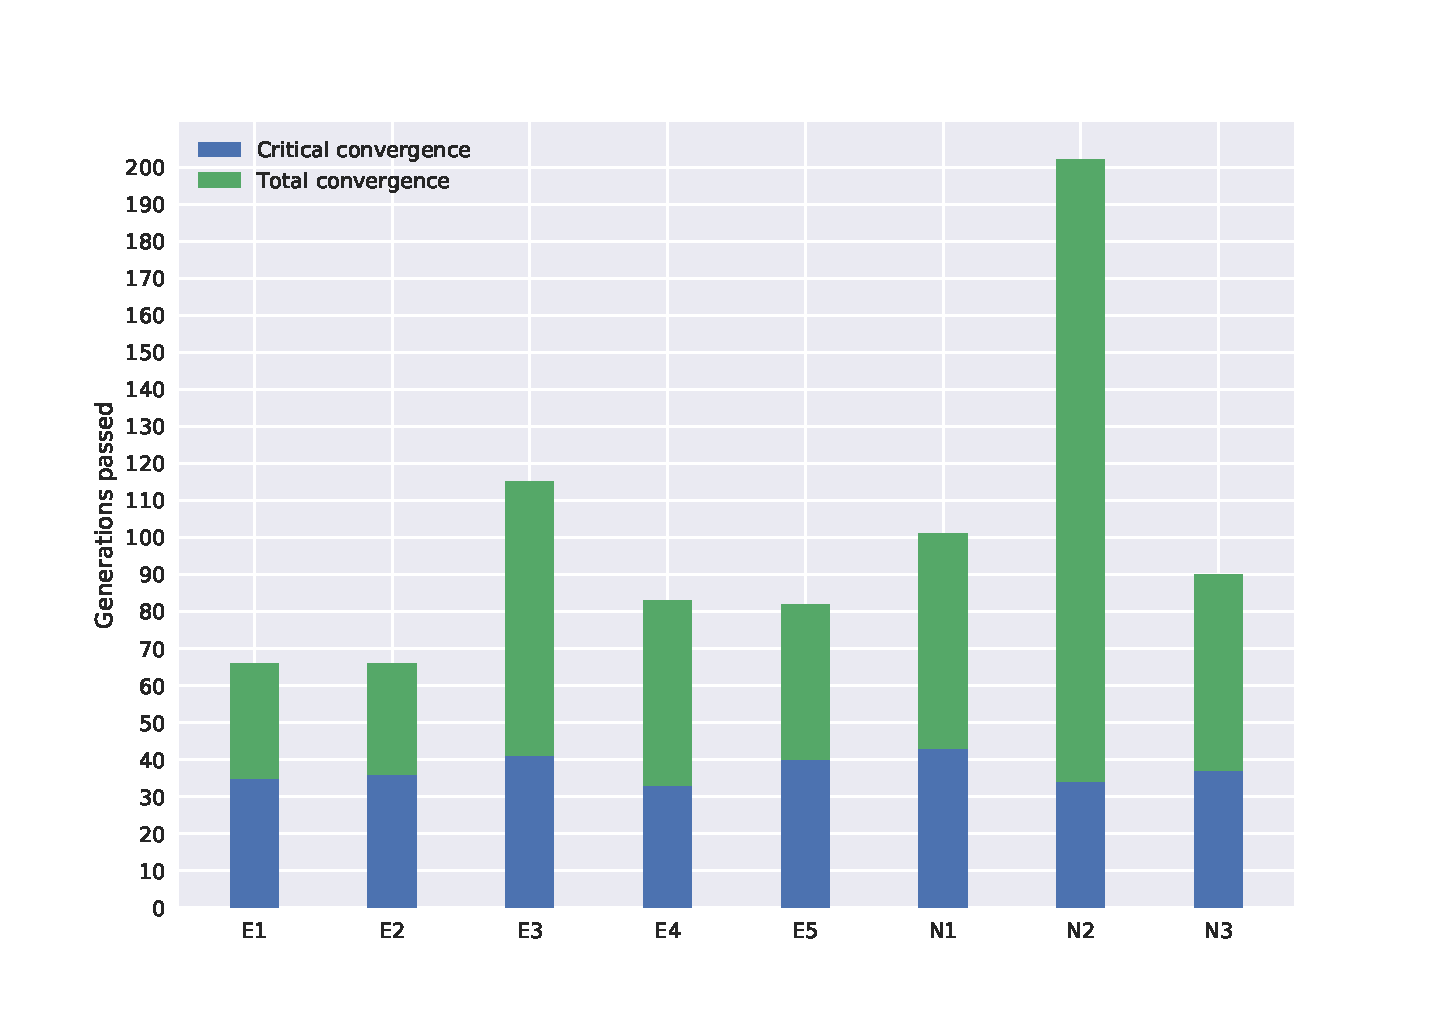
\includegraphics[width=310pt]{criticalcon1}
		\caption{Graph showing how many generations it took before reaching critical convergence (in blue), and how many generations there were before total convergence (in green).}
		\label{fig:criticalconv}
	\end{figure}
	\begin{table}[H]
		\centering
		\caption{Raw data for graph \ref{fig:criticalconv}}
		\label{table:criticalconv}
		\begin{tabular}{llllllll|r}
			\\
			\textbf{E1} & \textbf{E2} & \textbf{E3} & \textbf{E4} & \textbf{E5} & \textbf{N1} & \textbf{N2} & \textbf{N3} & \textbf{Average} \\ \hline \\
			35 & 36 & 41 & 33 & 40 & 43 & 34 & 37 & 37.375 \\
		\end{tabular}
	\end{table}
	\pagebreak
	\subsection{Critical parameters}
	Regarding to how many generations it takes to reach critical convergence we could observe that it is completely independent on how many total generations a optimization takes. The same can also be observed for how many parameters that are converged when reaching critical convergence, as seen in table \ref{table:criticalparams}. For the experiments with accelerated convergence (E) and those without (N) - there does not seem to be any significant disparity. With a sample standard deviation of 2.17, we get a confidence level of 68,3\% for results within 19.5 - 21.2 and 90\% within 19 - 21.7.
	\begin{table}[H]
		\centering
		\caption{How many parameters converged to reach estimated critical convergence.}
		\label{table:criticalparams}
		\begin{tabular}{llllllll|r}
			\\
			\textbf{E1} & \textbf{E2} & \textbf{E3} & \textbf{E4} & \textbf{E5} & \textbf{N1} & \textbf{N2} & \textbf{N3} & \textbf{Average} \\ \hline \\
			23 & 22 & 19 & 20 & 19 & 22 & 16 & 22 & 20.375 \\
		\end{tabular}
	\end{table}
	\clearpage
	\subsection{Accelerated convergence}
	Because of time constraints there is data from only three experiments without accelerated convergence active. This means that the data is somewhat lacking, especially due to a high variance in experiments without accelerated convergence, but a conclusion is still able to be drawn based on the data at hand, seen in figure \ref{fig:accon} and table \ref{table:accon}.
	\begin{figure}[H]
		\centering
		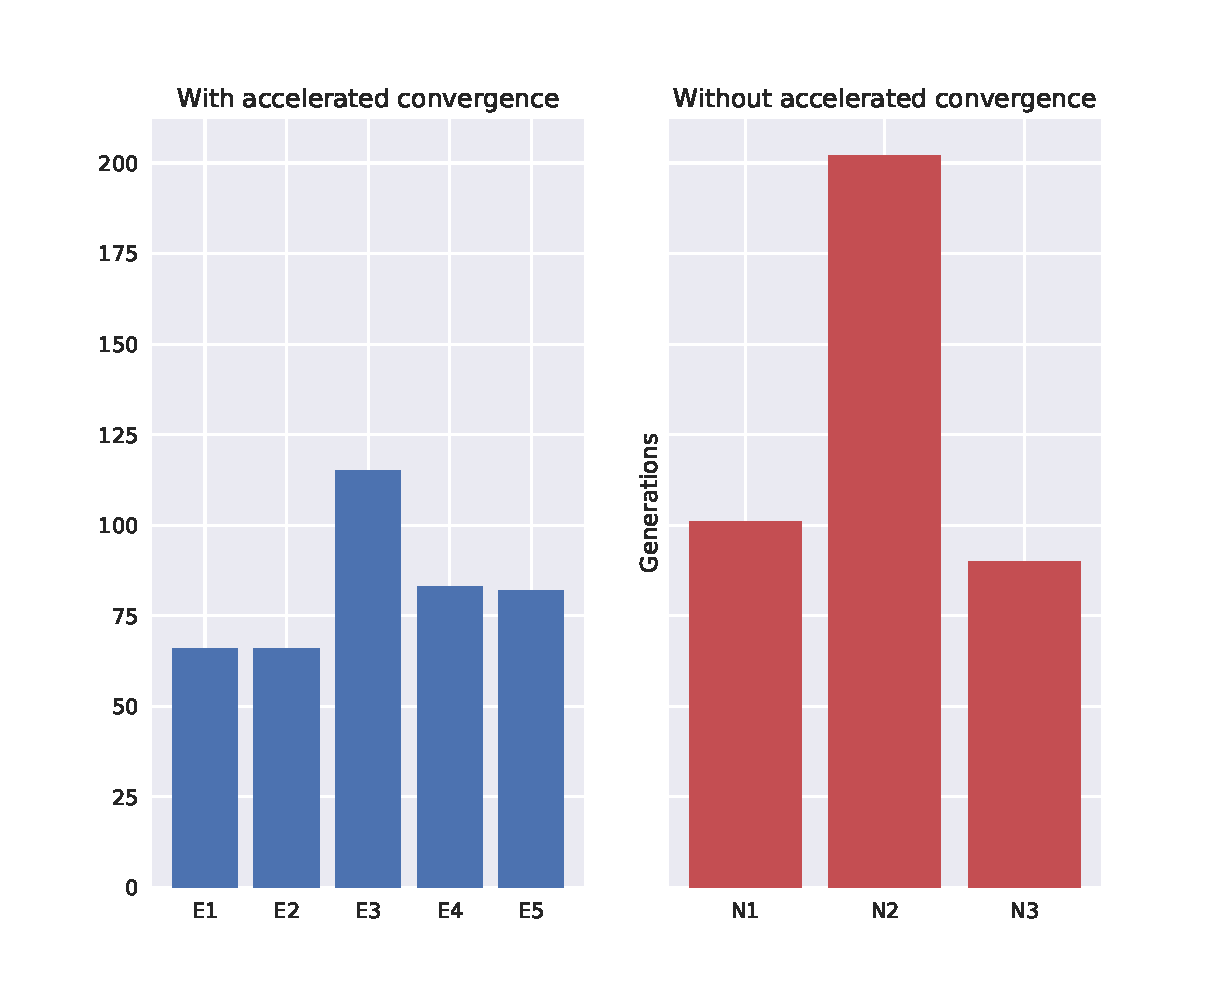
\includegraphics[width=310pt]{accon}
		\caption{Graph showing how many generations it took before reaching critical convergence (in blue), and how many generations there were before total convergence (in green).}
		\label{fig:accon}
	\end{figure}
	\begin{table}[H]
		\centering
		\caption{How many generations it took until convergence, with accelerated convergence (E) and without (N).}
		\label{table:accon}
		\begin{tabular}{lllll|r}
			\\
			\textbf{E1} & \textbf{E2} & \textbf{E3} & \textbf{E4} & \textbf{E5} & \textbf{Average} \\ \hline \\
			66 & 66 & 115 & 83 & 82 & 82.4 \\
		\end{tabular}
	\\[0.5\in]
	
		\begin{tabular}{lll|r}
		\\
		 \textbf{N1} & \textbf{N2} & \textbf{N3} & \textbf{Average} \\ \hline \\
		101 & 202 & 90 & 131 \\
		\end{tabular}
	\end{table}
	Average amount of generations with accelerated convergence was 82.4, and without it was 131. For accelerated jobs there's a sample standard deviation of 20, we get a confidence level of 68,3\% for results within 73.5 - 91.3 and 90\% within 67.7 - 97.1. For non accelerated tuns there's a sample standard deviation of 61.7, we get a confidence level of 68,3\% for results within 95.4 - 166.6 and 90\% within 72.4 - 189.6. Even though the amount of data is low, a considerable difference can be seen, at least indicating that accelerated convergence works. If we were to read this as is, the data shows that accelerated convergence on average decreases process time by 37\% - which is substantial.
	\subsection{Cost saving}
	\paragraph{TTE for solution assurance} For this section data from the total number of solution assurance jobs for all eight experiments will be visualized. This ensures a large set of data for accurate analysis.
	\begin{figure}[H]
		\centering
		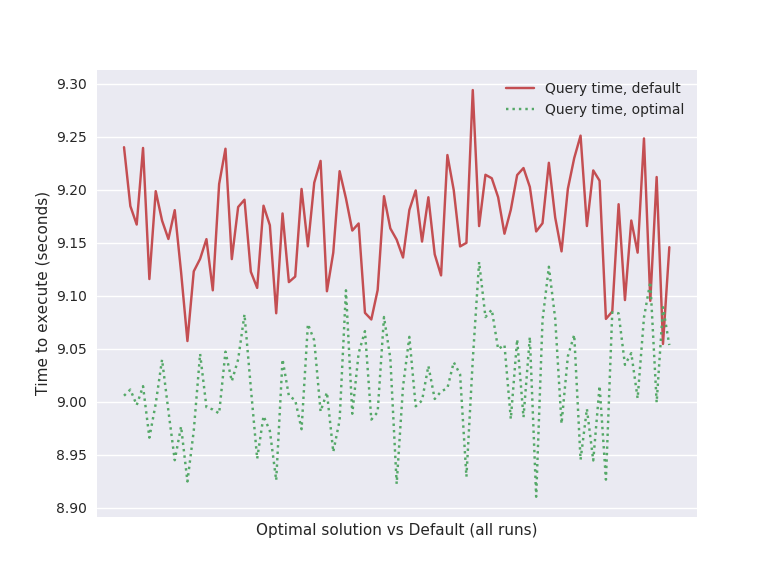
\includegraphics[width=\textwidth]{costsaving}
		\caption{All jobs from all solution assurance stages for each experiment.}
		\label{fig:costsaving}
	\end{figure}
	Figure \ref{fig:costsaving} shows that across almost all jobs, there is a cost saving, except for some data points where the default candidate is better. However this graph is hard to read, so figure \ref{fig:costsaving2} shows the same data sorted.
	\begin{figure}[H]
		\centering
		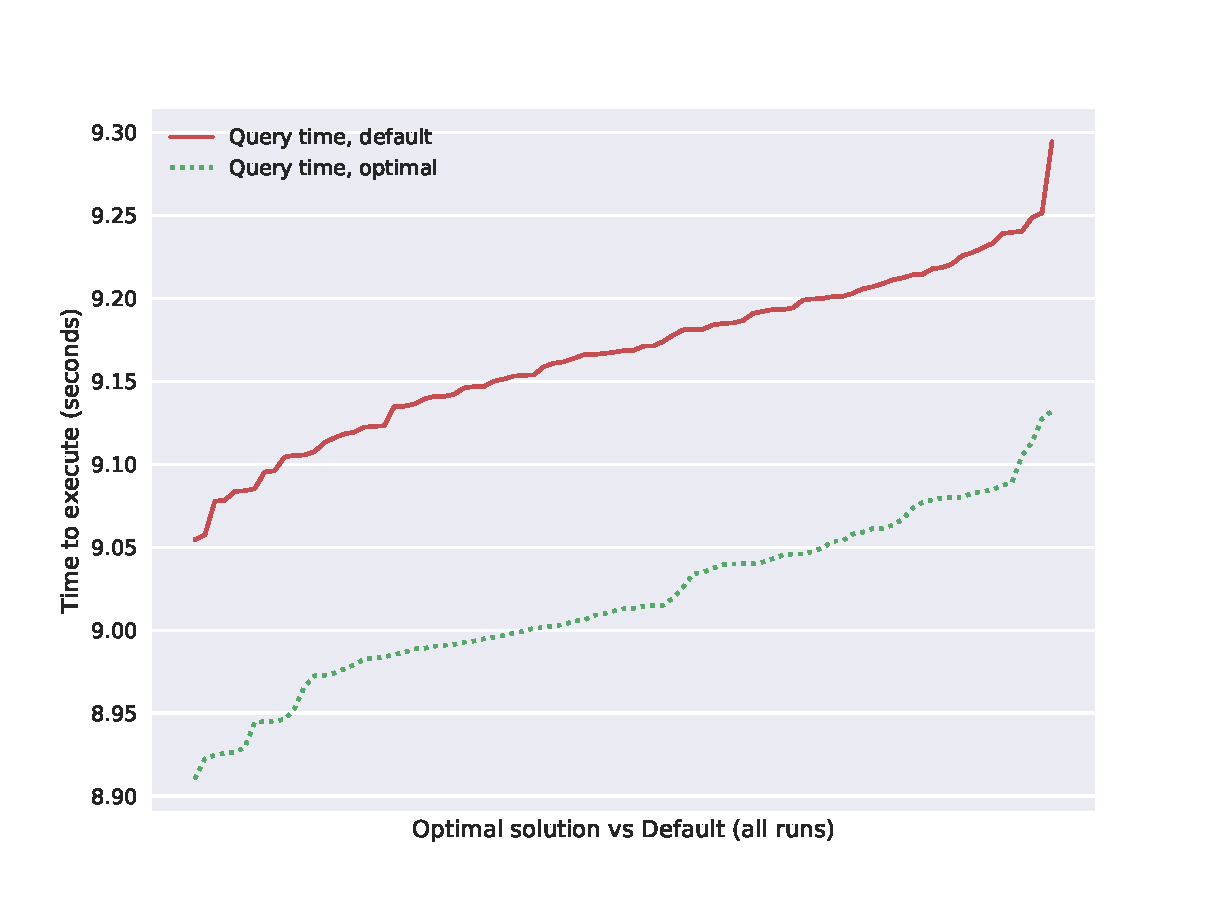
\includegraphics[width=\textwidth]{costsaving2}
		\caption{All jobs from all solution assurance stages for each experiment - sorted.}
		\label{fig:costsaving2}
	\end{figure}
	In figure \ref{fig:costsaving2} we can clearly see that the default candidate at its best, is better than the converged candidate solution at its worst. However there is a very symmetrical and steady disparity in the results, where the default candidate has 0.15s higher TTE across the board, confirmed by the calculated averages shown in table \ref{table:costsaving}.
	\begin{table}[H]
	\centering
	\caption{Summary of results for cost saving.}
	\label{table:costsaving}
	\begin{tabular}{ll|r}
		\\
		\textbf{Average default TTE} & \textbf{Average solution TTE} & \textbf{Cost saving} \\ \hline \\
		9.16 & 9.01 & 1,63\% \\
	\end{tabular}
\end{table}
	\chapter{Discussion}
	\section{The drill cache}
	\label{sec:cache}
		As mentioned previously, a candidate job consists of two stages - one concurrent stage and one sequential stage. A single job on a single candidate will always perform at least two sequential queries. All candidates in a population are run in sequence, one after the other whilst measuring their fitness. Still we see that the first job of the optimization process, running the default candidate, is measured to have higher TTE than subsequent jobs when performing solution assurance in the end - if the job count is low. This is caused by drill populating a distributed cache, which the default candidate will utilize fully in subsequent jobs, but not in the goal defining job. This source of deviance from the true performance of the default candidate is however irrelevant in the grand scheme, as the goal could be an arbitrary value to beat for the generated candidates. After all the algorithm does not end when a goal is reached, rather when convergence is achieved. When performing solution assurance in the end the true performance gets measured against the converged candidate solution, and a fair assessment of both candidates' TTE is made, proving effect - or lack thereof.
	\section{Parameter agnostic queries}
		\label{sec:param_agno}
		\subsection{Tiny queries, non-complex problems}
		Running a very simple query in the cluster environments we set up, on a small json file of a couple thousand lines - took drill around 0.2 seconds. Attempting to optimize for such queries was completely futile, as the only bottleneck for such a simple query is pure hard drive reading speeds. This led to every randomized set of settings to be considered equally good, which again means that the default candidate is equally good. No optimal solution can be discovered, and convergence of the algorithm is simply an act of chance.
		\pagebreak
		\subsection{Complex queries}
		As queries get more difficult to plan, the data set gets bigger, the cluster gets more heterogeneous and the data source more complex - the impact of performance tuning increases. As discussed previously drill has different phases when executing a query, like the logical and the physical planning phases. The planning phases heavily depend on the configuration settings and performance tuning parameters to calculate how to carry on execution of a query. We discovered early on that in a given environment there were some parameters that heavily impacted the execution time, and some others that were completely arbitrary, or even ignored by drill in runtime. This led to the creation of the accelerated convergence state in the knowledge object, to increase probability vector growth once the critical parameters have been sorted out.
		\subsection{Solution}
		After introducing accelerated convergence, we give the algorithm an extra push in the last 10\% towards convergence, to make sure we don't waste time and resources on a random gamble of irrelevant parameters to the current environment and / or data source. Convergence still takes a lot of time in case of heavy parameter agnosticism, but aborting the algorithm prematurely to force default options on the respective arbitrary parameters could lead to faulty configurations in edge cases, so we settled for speeding it up instead - with accelerated convergence.
		\clearpage
	\section{Error sources}
		\subsection{Drill planner inconsistency}
		First of all, drill is inherently a bit varied in terms of query times. Performing the same query twice in the same session will heavily leverage a shared cache amongst the drillbits, reducing query times by an average of 15\%. Further more the planning phase contains some fuzzy logic and decision making probabilities, so it may not always result in the same execution stage. The cache issue is mitigated by letting every candidate start a new session, and run the same amount of queries in the session. The planning stage inconsistency is mitigated by running several queries in a single job, to make sure to take the average into consideration. The solutions to both these problems are however parameterized, so setting the amount of queries per job to a low number will lead to increasing impact of these factors as error sources.
		\subsection{Cluster instability}
		In the initial testing phase, results from jobs varied widely in execution time. The cluster however, was a shared resource where many projects were competing for computing power. Even running only the default candidate for 50 generations, extreme spikes in TTE as high as 30\% were seen, randomly distributed amongst the jobs. When cluster instability gets added on top of drill planner inconsistency in a single query / job, it leads to an outlier of very high TTE. However with such variations it is hard to reach a sensible convergence for truly optimal solutions, considering how fitness scores then are products of both settings and circumstance. This led to a migration to a similar sized cluster of 4 nodes, but with a lower spec, where the resources where allocated and could not be competed for, hereby called the \hyperref[table:cluster_stable]{stable cluster}. The stable cluster mitigated the variations and gave good grounds for studying the result of the algorithm. 
		\subsection{Cluster size}
		Enterprise environments where optimization techniques like this would be most beneficial, are also the hardest ones to simulate. Increasing the amount of nodes and the amount of resources would add to the complexity, mitigating the optimization problem of parameter agnosticism. 
	\pagebreak
	\section{Proving effect}
	 After analyzing our data it is clear that the algorithm works as intended - reducing the overall TTE. It is proven across several solution assurance jobs that the average cost saving of the converged candidate solution is worthwhile, averaging out at 1,53\% for the \hyperref[table:cluster_stable]{stable cluster}, for the highlighted experiments. For the \hyperref[table:cluster_shared]{shared cluster} cost saving is inconclusive, because of the heavy variance in TTE caused by the shared resources, leading to faulty results.
	\section{Cut configuration parameters}
	Time constraints and choice of implemented algorithm caused some relevant parameters to be cut from the optimization process, making them default values in all candidates. There were a total of six cut parameters, viewable in the appendix, \hyperref[table:removed_params]{cut parameters}. The two execution queue memory parameters could not be set in-session, as they were exclusively system settings. This meant that we would need to restart apache for each candidate, to apply their system settings, causing massive overhead and added complexity. The four remaining ones all define what type of aggregation and join functions should be available. Changing these parameters led to segmentation faults while running candidates, and they then had to be cut from the settings list. Given more time, some deeper study and insight could be gained to understand the segmentation faults, and perhaps build systems to handle them.
	
	\chapter{Further work}
	\section{Homogeneous clusters}
	In this thesis both the clusters set up consisted of a homogeneous set of nodes. It is expected that a heterogeneous cluster will have added complexity to the logical and physical planner on the drillbits, further increasing the value of optimization. This is a high priority effort for future work, as it accurately represents a real world use case.
	\subsection{Load profiles}
	It should be infeasible for one configuration to solve all problems. After all, the concept of optimization takes great consideration to its specific context. Expecting to solve all aspects of a complex problem with one remedy leads to a candidate being a jack of all trades but master of none. Hence the solution should be tailored to a specific context, by letting the algorithm aggressively tune the system to work in its current state. To make sure this algorithm performs this way, testing needs to be done on different kinds of data sets, with different kinds of queries.
	\section{Single node setups}
	It would be interesting to gather data from a single node laptop setup for running queries in drill. The way data sources work in this thesis through pyodbc meant that it would add too much development time to adapt for local hard drive jobs, either in the way of configuring a hard drive location as an ODBC DSN, or altering the way we programatically perform drill queries. 
	\pagebreak
	\section{Support for the cut parameters}
	As mentioned earlier there are a couple of interesting parameters that was cut from the development process in this thesis, listed in \hyperref[table:removed_params]{the appendix}. To handle the segmentation faults potentially caused by hash- and aggregate join disabling, one could possibly access drill through a different source than pyodbc, to create an appropriate wrapper around the jobs and catch the errors. To handle the system settings, a more complex process needs to be set up, to restart the cluster and check for readiness before querying it for each candidate - this may ultimately be infeasible in terms of optimization time.
	
	\chapter{Conclusion}
	\section{Innovation - SIILCK}
		\subsection{Inspiration}
		This thesis started out using a simple Genetic Algorithm for the candidate solutions. Further in the development process PBIL was implemented, as a better fit for the object oriented authority based system made, with the society at the top. Even still some alterations to the algorithm had to be made to reach the intended goal, and thus PBIL was not satisfactory. This led to the creation of a new algorithm named SIILCK.
		\subsection{Genetic flexibility}
		SIILCK accepts any type of structure as a solution, from numbers and strings to complex values like lists and matrices. The parameter options can even be objects themselves. This is all handled by using the knowledge object held by the society, that mirrors the parameters held by the candidates, representing them as a probability vector. The flexibility in parameter options is a considerable improvement over traditional genetic algorithms, which purely allow for binary genetic material.
		\subsection{Mutation}
		Genetic algorithms mutate candidates. PBIL mutates the collective probability vectors. SIILCK mutates on candidate level, potentially allowing an advantageous mutated candidate to reach academic status, thus altering the collective probability vector. In such a way SIILCK combines the methods presented in both GA and PBIL.
		\clearpage
		\section{Goal}
		\subsection{Self optimizing system}
		SIILCK is by every definition a self optimizing system. A user of the algorithm simply need to define a goal, how many parameters a solution object should have, and what options they should contain, to solve a given problem. The rest is up to the Society.
		\subsection{Apache drill performance tuning}
		With an average of 1.63\% cost saving in the testbed environment on a static query upon a large JSON dataset in a distributed file system, we consider it a success. Further more the algorithm will work in any environment and with any data type or data skewness due to the search based nature of SIILCK, as with other search based evolutionary algorithms like GA or PBIL.
		\section{Valuable contribution}
		The most valuable contribution of this thesis lies in the algorithm SIILCK, which can be used to solve several complex problems, improving upon traditional evolutionary algorithms with a major increase in genetic material flexibility, with an easy-to-grasp and relatable concept. It is also worth mentioning that this is the first ever tailor-made Apache Drill self optimization system, ensuring users can optimize their cluster without in-depth domain knowledge.
	\begin{thebibliography}{1}
		\bibitem{mronline}
		Li, M., Zeng, L., Meng, S., Tan, J., Zhang, L., Butt, A. R., \& Fuller, N. (2014, June). \emph{Mronline: Mapreduce online performance tuning. In Proceedings of the 23rd international symposium on High-performance parallel and distributed computing (pp. 165-176).} ACM.
		\bibitem{gunther}
		Liao, G., Datta, K., \& Willke, T. L. (2013, August). \emph{Gunther: Search-based auto-tuning of mapreduce.} In European Conference on Parallel Processing (pp. 406-419). Springer Berlin Heidelberg.
		\bibitem{bmc}
		BMC Software, Inc (2018, January) \emph{http://www.bmc.com/guides/hadoop-examples.html}
		\bibitem{yarn}
		Apache Software Foundation (January 2018) \emph{https://hadoop.apache.org/docs/stable/hadoop-yarn/hadoop-yarn-site/YARN.html}
		\bibitem{starfish}
		Herodotou, H., Lim, H., Luo, G., Borisov, N., Dong, L., Cetin, F. B., \& Babu, S. (2011, January). \emph{Starfish: A Self-tuning System for Big Data Analytics.} In Cidr (Vol. 11, No. 2011, pp. 261-272).
		\bibitem{unixodbc}
		Nick Gorham (2018, February) \emph{http://www.unixodbc.org/}
		\bibitem{pyodbc}
		Michael Kleehammer (2018, February) \emph{https://github.com/mkleehammer/pyodbc}
		\bibitem{hadoopguide}
		White, T. (2012). \emph{Hadoop: The definitive guide.} " O'Reilly Media, Inc.".
		\bibitem{dremel}
		Melnik, S., Gubarev, A., Long, J. J., Romer, G., Shivakumar, S., Tolton, M., \& Vassilakis, T. (2010). \emph{Dremel: interactive analysis of web-scale datasets.} Proceedings of the VLDB Endowment, 3(1-2), 330-339.
		\bibitem{gfs}
		Ghemawat, S., Gobioff, H., \& Leung, S. T. (2003). \emph{The Google file system} (Vol. 37, No. 5, pp. 29-43). ACM.
		\bibitem{mapredoriginal}
		Dean, J., \& Ghemawat, S. (2008). \emph{MapReduce: simplified data processing on large clusters.} Communications of the ACM, 51(1), 107-113.
		\bibitem{dremelcustomers}
		Google LLC (2018, February) \emph{https://cloud.google.com/customers/}
		\bibitem{modis}
		Modis (2018, February) \emph{http://www.modis.com/it-insights/infographics/top-it-jobs-of-2018/}
		\bibitem{own}
		Johannessen, R., Yazidi, A., \& Feng, B. (2017, April). \emph{Hadoop MapReduce scheduling paradigms. In Cloud Computing and Big Data Analysis} (ICCCBDA), 2017 IEEE 2nd International Conference on (pp. 175-179). IEEE.
		\bibitem{nasa}
		Hornby, G., Globus, A., Linden, D., \& Lohn, J. (2006). \emph{Automated antenna design with evolutionary algorithms.} In Space 2006 (p. 7242).
		\bibitem{drill}
		Apache Software Foundation (2018, January) \emph{https://drill.apache.org/docs/analyzing-the-yelp-academic-dataset/}
		\bibitem{joinplanning}
		Apache Software Foundation (2018, January)
		\emph{https://drill.apache.org/docs/join-planning-guidelines/}
		\bibitem{drill_releases}
		Apache Software Foundation (2018, February) 	\emph{https://drill.apache.org/docs/release-notes/}
		\bibitem{impedance}
		Ireland, C., Bowers, D., Newton, M., \& Waugh, K. (2009, March). \emph{A classification of object-relational impedance mismatch.} In Advances in Databases, Knowledge, and Data Applications, 2009. DBKDA'09. First International Conference on (pp. 36-43). IEEE.
		\bibitem{bettercloud}
		2018 BetterCloud Monitor (2018, February)
		\emph{https://www.bettercloud.com/monitor/real-time-enterprise-messaging-comparison-data/}
		\bibitem{humangenome}
		Stack Exchange Inc, posted by user: Thoth (2018, February) \emph{https://stackoverflow.com/questions/42403229/mysql-database-with-thousands-of-tables}
		\bibitem{bigdata}
		Gantz, J., \& Reinsel, D. (2012). \emph{The digital universe in 2020: Big data, bigger digital shadows, and biggest growth in the far east.} IDC iView: IDC Analyze the future, 2007, 1-16
		\bibitem{servicemax}
		Porter, M. E., \& Heppelmann, J. E. (2015). \emph{How smart, connected products are transforming companies.} Harvard Business Review, 93(10), 96-114.
		\bibitem{management_analytics}
		Bendre, M. R., \& Thool, V. R. (2016). \emph{Analytics, challenges and applications in big data environment: a survey.} Journal of Management Analytics, 3(3), 206-239.
		\bibitem{future_data}
		Huang, G., He, J., Chi, C. H., Zhou, W., \& Zhang, Y. (2015, June). \emph{A Data as a Product Model for Future Consumption of Big Stream Data in	Clouds.} In 2015 IEEE International Conference on Services Computing (SCC), (pp. 256-263). IEEE.
		\bibitem{statista}
		Statista, Inc (2018, February) \emph{https://www.statista.com/statistics/ + [266206/googles-annual-global-revenue/, 277229/facebooks-annual-revenue-and-net-income/]}
		\bibitem{no_sql}
		Github user Edlich, curated list (2018, February) \emph{http://nosql-database.org/}
		\bibitem{pbil}
		Baluja, S. (1994). \emph{Population-based incremental learning. a method for integrating genetic search based function optimization and competitive learning} (No. CMU-CS-94-163). Carnegie-Mellon Univ Pittsburgh Pa Dept Of Computer Science.
		\bibitem{impala}
		Bittorf, M. K. A. B. V., Bobrovytsky, T., Erickson, C. C. A. C. J., Hecht, M. G. D., Kuff, M. J. I. J. L., Leblang, D. K. A., ... \& Yoder, M. M. (2015). \emph{Impala: A modern, open-source SQL engine for Hadoop.} In Proceedings of the 7th Biennial Conference on Innovative Data Systems Research.
		\bibitem{impalasite}
		Apache Software Foundation (2018, March) 
		\emph{https://impala.apache.org/overview.html}
		\bibitem{spark_ml}
		Meng, X., Bradley, J., Yavuz, B., Sparks, E., Venkataraman, S., Liu, D., ... \& Xin, D. (2016). \emph{Mllib: Machine learning in apache spark.} The Journal of Machine Learning Research, 17(1), 1235-1241.
		\bibitem{yelp}
		 Yelp Inc. Yelp (2018, March)
		\emph{https://www.yelp.com/dataset/challenge}
		\bibitem{globalknowledge}
		 Global Knowledge Training LLC. (2018, March)\\
		 Big Data and Apache Hadoop Adoption: Key Challenges and Rewards
		\emph{https://www.globalknowledge.com/us-en/content/articles/big-data-and-apache-hadoop-adoption/}
		\bibitem{siliconA}
		SiliconANGLE Media, Inc. (2018, March)
		\emph{https://siliconangle.com/blog/2012/08/01/hadoop-big-data-reports-future-growth/}
		\bibitem{Gartner}
		Gartner, Inc, Gartner Survey Highlights Challenges to Hadoop Adoption
		\emph{https://www.gartner.com/newsroom/id/3051717} STAMFORD, Conn., May 13, 2015
		\bibitem{mapr_drill}
		MapR Technologies, Inc. (2018, March)
		\emph{https://mapr.com/blog/apache-drill-architecture-ultimate-guide/}
	\end{thebibliography}

\appendix
\chapter{Cluster specs}
\begin{table}[H]
	\centering
	\caption{Specs for the shared cluster}
	\label{table:cluster_shared}
	\begin{tabular}{ll}
		\\
		\multicolumn{1}{l}{\bfseries Specification} & \multicolumn{1}{l}{\bfseries Value} \\ \hline \\
		Amount of nodes & 4  \\
		Heterogeneous & No  \\
		OS & Ubuntu 17.10  \\
		VCPUs & 4  \\
		RAM & 8GB  \\ 
		HDD & 80GB  \\
	\end{tabular}
\end{table}

\begin{table}[H]
	\centering
	\caption{Specs for the stable cluster}
	\label{table:cluster_stable}
	\begin{tabular}{ll}
		\\
		\multicolumn{1}{l}{\bfseries Specification} & \multicolumn{1}{l}{\bfseries Value} \\ \hline \\
		Amount of nodes & 4  \\
		Heterogeneous & No  \\
		OS & Ubuntu 16.04  \\
		VCPUs & 2  \\
		RAM & 2GB  \\ 
		HDD & 15GB  \\
	\end{tabular}
\end{table}

\chapter{System parameters}
\label{system_params}
\begin{table}[H]
	\centering
	\caption{All parameters and options used by PBIL in this thesis}
	\label{table:added_params}
	\begin{tabular}{ll}
		\\
		\multicolumn{1}{l}{\bfseries Name} & \multicolumn{1}{l}{\bfseries Default value} \\ \hline \\
		planner.memory.enable\_memory\_estimation & False  \\
		exec.queue.enable & False  \\
		planner.broadcast\_factor & 1  \\
		planner.broadcast\_threshold & 10000000  \\
		planner.slice\_target & 1000  \\
		planner.width.max\_per\_query & 1000  \\
		exec.min\_hash\_table\_size & 65536  \\
		exec.max\_hash\_table\_size & 1073741824  \\
		exec.queue.large & 10  \\
		exec.queue.small & 100  \\
		exec.queue.threshold & 30000000  \\
		exec.queue.timeout\_millis & 300000  \\
		planner.memory.max\_query\_memory\_per\_node &  max\_query\_memory  \\
		planner.width.max\_per\_node & calculated  \\
		planner.add\_producer\_consumer & False  \\
		planner.enable\_hashjoin\_swap & True  \\
		planner.enable\_mergejoin & True  \\
		planner.filter.max\_selectivity\_estimate\_factor & 1  \\
		planner.filter.min\_selectivity\_estimate\_factor & 0  \\
		planner.join.hash\_join\_swap\_margin\_factor & 10  \\
		planner.join.row\_count\_estimate\_factor & 1  \\
		planner.memory.average\_field\_width & 8  \\
		planner.memory.hash\_agg\_table\_factor & 1.1  \\
		planner.memory.hash\_join\_table\_factor & 1.1  \\
		planner.memory.non\_blocking\_operators\_memory & 64  \\
		planner.partitioner\_sender\_max\_threads & 8  \\
		planner.nestedloopjoin\_factor & 100  \\
		planner.producer\_consumer\_queue\_size & 10  \\
		store.text.estimated\_row\_size\_bytes & 100  \\
	\end{tabular}
\end{table}

\begin{table}[H]
	\centering
	\caption{Parameters and options that was removed during development, but still is considered to have impact on performance of query execution}
	\label{table:removed_params}
	\begin{tabular}{ll}
		\\
		\multicolumn{1}{l}{\bfseries Name} & \multicolumn{1}{l}{\bfseries Default value} \\ \hline \\
		planner.enable\_multiphase\_agg & True  \\
		planner.enable\_broadcast\_join & True  \\
		planner.enable\_hashagg & True  \\
		planner.enable\_hashjoin & True  \\
		exec.queue.memory\_ratio & 10  \\ 
		exec.queue.memory\_reserve\_ratio & 0.2  \\
	\end{tabular}
\end{table}

\chapter{Configuration parameters}
\begin{table}[H]
	\centering
	\caption{Configuration parameters that define how the algorithm executes.}
	\label{table:conf_params}
	\begin{tabular}{ll}
		\\
		\multicolumn{1}{l}{\bfseries Name} & \multicolumn{1}{l}{\bfseries Default value} \\ \hline \\
			POPULATION\_SIZE& 10 \\
			GROWTH\_FACTOR & 0.4 \\
			GROWTH\_CHANCE & 0.3 \\
			RESISTANCE & 0.1 \\
			
			CONVERGENCE\_THRESHOLD & 0.95 \\
			MAX\_GENERATIONS & 200 \\
			CONCURRENT\_RUNS & 10 \\
			
			REPLACEMENTS\_EACH\_RUN & 5 \\
			ELITES\_EACH\_RUN & 3 \\
			ELITE\_CLUB\_SIZE & 7 \\
			
			DATA\_SOURCE & drill64 \\
			NODES & 4 \\
			CORES & 4 \\
			NODE\_LEAST\_MEMORY & 2147483648 \\
			
			DISPLAY\_OUTPUT & false \\
			LOGGING\_FOLDER & /home/ubuntu/runlogs/ \\
			RUN\_NAME & default \\
	\end{tabular}
\end{table}

\chapter{Code}
\section{Introduction}
This thesis code directory contains 6 subdirectories with a total of 51 files within. A lot of files are scripts to help set up the cluster, many of them are configuration files that define the cluster, and some are code directly related to SIILCK and the optimization process. The code directly related to SIILCK and the optimization process is the code we chose to display in this chapter. Please view the attached code mostly as a contingency in case the public repo goes down, as it is hard to read in this format. To view the full extent and complexity of the project, nicely formatted, please visit the public GitLab page on this address:
\\
\\
\href{https://gitlab.com/blawtekjar/master-thesis-code/tree/pbil}{https://gitlab.com/blawtekjar/master-thesis-code/tree/pbil}
\\
\\
Specifically the directory named \textbf{pydrill}, which contains all the code from this chapter.
\\
\\
Furthermore the code displayed does not follow the naming convention of the main thesis, as the high level abstractions and metaphors were refined as development carried on. For those that want to study the code the translated names are:
\begin{table}[H]
	\centering
	\caption{Differences in naming from SIILCK as covered in thesis and objects in attached code.}
	\label{table:code_names}
	\begin{tabular}{ll}
		\\
		\multicolumn{1}{l}{\bfseries SIILCK name} & \multicolumn{1}{l}{\bfseries Code name} \\ \hline \\
		Society& Judge \\
		Knowledge & Memory \\
		Setting & Solution \\
		Candidate & Candidate \\
		Job & Run \\
		Academia & Elite\_club \\
		Academic & Elite \\
	\end{tabular}
\end{table}
\section{Repository file overview}
\begin{figure}[H]
	\centering
	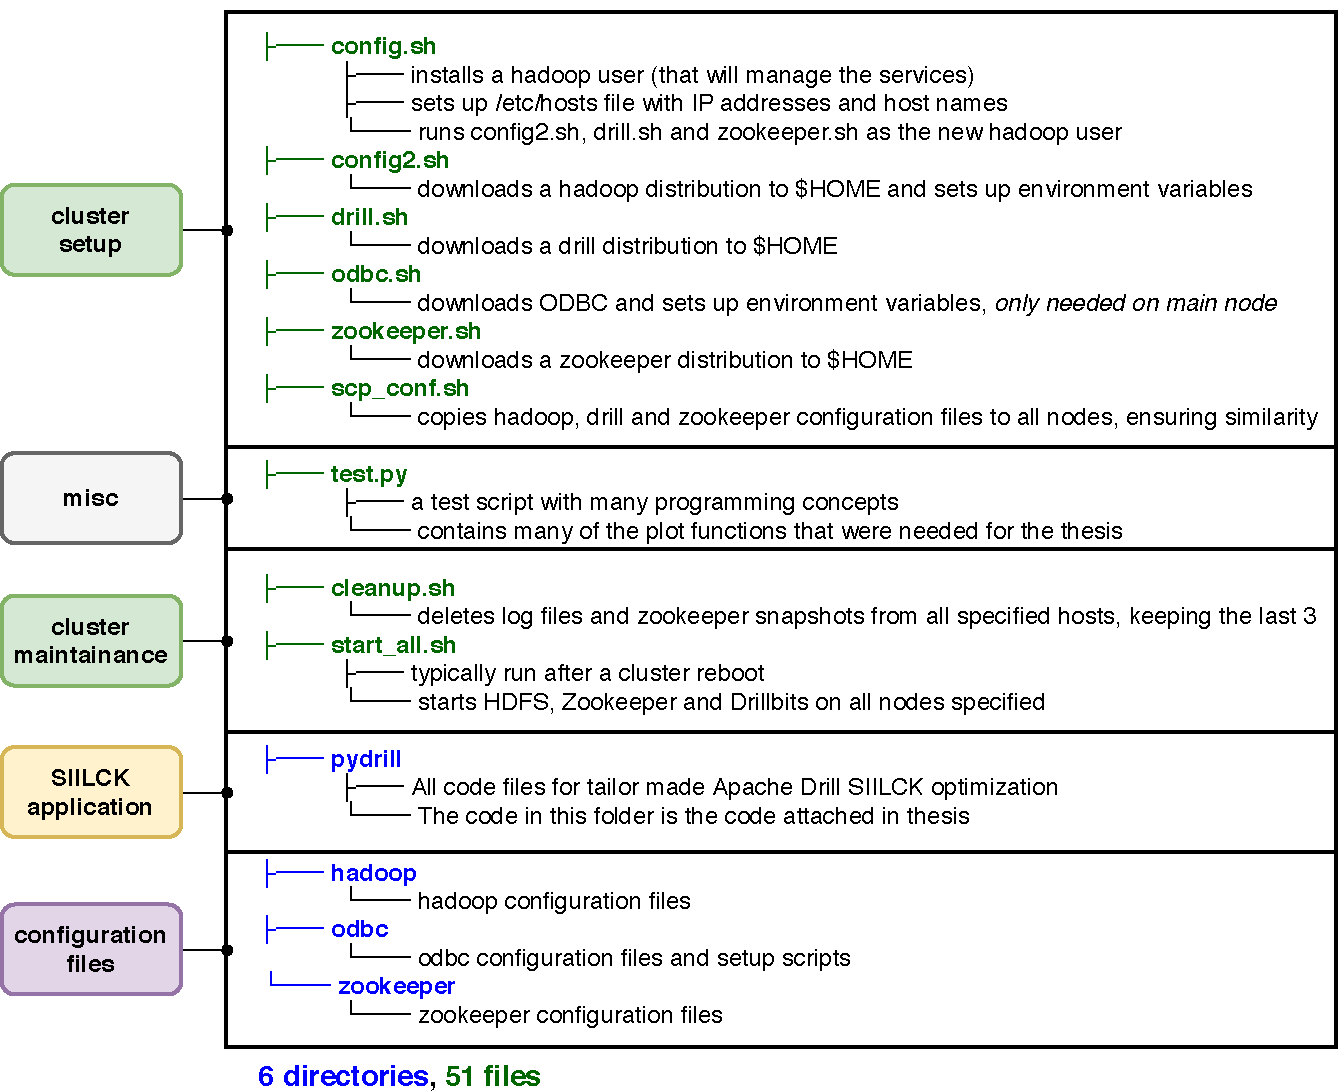
\includegraphics[width=\textwidth]{repo_tree}
	\caption{All files and directories within the repository, and a brief description of their purpose.}
	\label{fig:repotree}
\end{figure}
\pagebreak
\section{config.py}
This is the script that starts a process. It can be run with flags:
\begin{table}[H]
	\centering
	\caption{config.py execution flags.}
	\label{table:config_flags}
	\begin{tabular}{p{4cm}p{7cm}}
		\\
		\multicolumn{1}{l}{\bfseries flag} & \multicolumn{1}{l}{\bfseries effect} \\ \hline \\
		-name:\$NAME& Choose name for process. Data will then be logged to logging folder specified in config.json, in a directory of the chosen \$NAME. If no name is chosen the default name is specified within config.json.' \\
		\\
		-display & Shows all output of queries ran, which is usually hidden as the act of displaying the results wastes time. \\
		\\
		-concurrent:\$NUM & Overrides the CONCURRENT\_RUNS setting from config.json to manually choose \$NUM amount of queries to perform. Can for instance be set to 1 to perform a quick cluster test run without altering the config file.  \\
	\end{tabular}
\end{table}
\begin{lstlisting}[language=Python, caption=config.py. The file we run to start a process]
#!/usr/bin/python3

import sys
import os
import class_definition
import json
from plotting import store_run
from datetime import datetime

# Get config
with open('config.json') as json_data:
data = json.load(json_data)

# Can be overwritten by cli args
CONCURRENT_RUNS = data["CONCURRENT_RUNS"]
DISPLAY_OUTPUT = data["DISPLAY_OUTPUT"]
RUN_NAME = data["RUN_NAME"]

# Check CLI args
for arg in sys.argv:
if arg == "-display":
DISPLAY_OUTPUT = True
if arg.startswith("-concurrent"):
mylist = arg.split(":")
CONCURRENT_RUNS = int(mylist[1])
if arg.startswith("-name"):
mylist = arg.split(":")
RUN_NAME = mylist[1]


timestamp = datetime.now().strftime('%Y.%m.%d.%H.%M.%S')
path = data["LOGGING_FOLDER"]+RUN_NAME
count = 0
converged = False

judge = class_definition.Judge(data["POPULATION_SIZE"],
data["NODES"],
data["CORES"],
data["DATA_SOURCE"],
CONCURRENT_RUNS,
DISPLAY_OUTPUT,
data["GROWTH_FACTOR"],
data["GROWTH_CHANCE"],
data["RESISTANCE"],
data["CONVERGENCE_THRESHOLD"],
data["ELITE_CLUB_SIZE"],
data["ELITES_EACH_RUN"],
data["NODE_LEAST_MEMORY"])

while not converged:
try:
judge.run_candidates()
converged = judge.evolve_population(data["REPLACEMENTS_EACH_RUN"])

except Exception as e:
judge.log_error(e,data["LOGGING_FOLDER"],timestamp+RUN_NAME,judge.current_candidate)

finally:
count += 1
if count > data["MAX_GENERATIONS"]:
converged = True
print("MAX GENERATIONS REACHED")

if converged:
if not os.path.exists(path):
os.makedirs(path)
judge.settle_scores(path,timestamp)
store_run(judge,path,timestamp)
print("\n###############################")
print("############ Done! ############")
print("###############################\n\n")
else:
print("ERROR!! Check errorlog in "+data["LOGGING_FOLDER"])
\end{lstlisting}

\section{class\_definition.py}
In this file all SIILCK components are declared and used, and all functions defined. As mentioned previously some naming conventions are different than explained during the method chapter, and can be viewed in table \ref{table:code_names}.
\begin{lstlisting}[language=Python, caption=class\_definition.py\, the file defining all the algorithmic operations done during a optimization process.]

import random, sys
from threading import Thread
from statistics import mean
from connection import connect_z, execute_q, execute_query_sequence
from color import Color
from tabulate import tabulate
import numpy as np
import sklearn.linear_model as skl
from math import ceil
import os
from decimal import Decimal

class Judge:

elite_club = []

def settle_scores(self,log_location,timestamp):
self.run_candidates()
self.winner = self.get_fittest()
tab = []
for x in range(len(self.winner.settings.core_settings)):
tab.append([self.winner.settings.core_settings[x]["name"],
self.default_candidate.settings.core_settings[x]["query_value"],
self.winner.settings.core_settings[x]["query_value"],
self.memory.get_confidence(x)])
for x in range(len(self.winner.settings.extended_settings)):
tab.append([self.winner.settings.extended_settings[x]["name"],
self.default_candidate.settings.extended_settings[x]["query_value"],
self.winner.settings.extended_settings[x]["query_value"],"100%"])
formatted_string = tabulate(tab,headers=["Setting",
"Default value",
"Optimal value",
"Confidence"])
print(formatted_string)
self.confirm_solution()
with open(log_location+"/log.txt", "a") as myfile:
myfile.write("\n#### RUN: "+timestamp+"\n"+formatted_string+"\n")


def __init__(self,pop_size,nodes,cores,dsn,conc,disp,growth_factor,growth_chance,resistance,convergence_threshold,elite_club_size,elites_each_run,least_mem):
# Everything is kept within the judge as the judges own variables.
# This makes it easier to adapt the logging / plotting stage for future work.
self.dsn = dsn
self.conc = conc
self.disp = disp
self.nodes = nodes
self.cores = cores
self.least_mem = least_mem
self.accelerated = False
self.convergence_threshold = convergence_threshold 

self.resistance = resistance
self.growth_chance = growth_chance
self.growth_factor = growth_factor
self.population_size = pop_size
self.elite_club_size = elite_club_size
self.elites_each_run = elites_each_run

self.generation = 0
self.generations = {}
self.generations["upper"] = []
self.generations["lower"] = []
self.generations["mean"] = []
self.generations["fitness"] = []

self.memory = Memory(self.nodes,self.cores,self.least_mem)
self.default_candidate = Candidate(self.nodes,self.cores,self.least_mem,self.memory,name="Default candidate",default=True) 
self.current_candidate = self.default_candidate

self.define_goal(self.default_candidate)
self.generate_population()


def define_goal(self,candidate):
candidate.run(self.conc,self.disp,self.dsn)
self.goal = candidate.min_query * 0.5 # Quite arbitrary, but set for testing purposes?
self.benchmark = candidate.min_query

# TODO: Make fitness evaluation more sophisticated
def evaluate_fitness(self,candidate):
candidate.fitness = self.goal / candidate.min_query
candidate.cost_saving = format((1-(candidate.min_query/self.benchmark))*100,'.2f')

def generate_population(self):
print("Generating original population")
candidate_cage = []
for x in range(self.population_size):
candidate_cage.append(Candidate(self.nodes,self.cores,self.least_mem,self.memory,name="Candidate "+str(self.generation)+"."+str(x))) 
self.candidate_cage = candidate_cage

def run_candidates(self):
c = Color()
print(c.OKGREEN+"############ Testing generation "+str(self.generation)+" ############"+c.ENDC)
if self.accelerated:
print("Accelerated convergency active")
self.generation += 1
for c in self.candidate_cage:
self.current_candidate = c
c.run(self.conc,self.disp,self.dsn)
self.evaluate_fitness(c)

def execute_weakest(self,executions):
for x in range(executions):
lowest_fitness = 1
for c in self.candidate_cage:
if c.fitness < lowest_fitness:
lowest_fitness = c.fitness
weak_link = c
print("Killing off "+weak_link.name)
self.candidate_cage.remove(weak_link)

def let_strongest_into_the_club(self,births):
elites = []
for x in range(self.elites_each_run):
elites.append(self.get_fittest(exclusion=elites))
for elite in elites:
self.elite_club.append(elite)
self.generations["upper"].append(elite.max_query)
self.generations["lower"].append(elite.min_query)
self.generations["mean"].append(elite.mean_query)
self.generations["fitness"].append(elite.cost_saving)
if len(self.elite_club) > self.elite_club_size:
self.elite_club = self.elite_club[-self.elite_club_size:] # Keep the elite club at predefined size
self.memory.refine_memory(self.elite_club,self.growth_factor)
for x in range(births):
print("Adding new Candidate: "+str(self.generation)+"."+str(x))
c = Candidate(self.nodes,self.cores,self.least_mem,self.memory,name="Candidate "+str(self.generation)+"."+str(x)) 
c.mutate_settings(self.growth_factor,self.growth_chance,self.resistance)
self.candidate_cage.append(c)

def evolve_population(self,replacements):
self.execute_weakest(replacements)
self.let_strongest_into_the_club(replacements)
converged, con = self.memory.check_for_convergence(self.convergence_threshold)
if con > self.convergence_threshold*0.9 and not self.accelerated:
self.accelerated = True
self.growth_factor += 0.2
self.memory.estimate_time(self.convergence_threshold)
return converged

def log_error(self,error,log_location,timestamp,c):
self.candidate_cage.remove(c)
print("Error caught in candidate "+c.name+", replaced")
self.candidate_cage.append(Candidate(self.nodes,self.cores,self.least_mem,self.memory,name="Candidate "+str(self.generation)+".replacement")) 
with open(log_location+"error_log.txt", "a") as myfile:
myfile.write("\n#### ERROR WITH THIS RUN: "+timestamp+"\n")
myfile.write(str(error))

def get_fittest(self,exclusion=[]):
highest_fitness = 0
for c in self.candidate_cage:
if c not in exclusion:
if c.fitness > highest_fitness:
highest_fitness = c.fitness
fittest = c
return fittest

def confirm_solution(self):
c = Color()
os.system('clear')
print("\n###############################")
print("########## Optimizing #########")
print("###############################\n\n")
print(c.OKGREEN+"\nOptimal settings has been chosen, confirming solution."+c.ENDC)
winner_mean = [self.winner.mean_query]
winner_max = [self.winner.max_query]
winner_min = [self.winner.min_query]

default_mean = [self.default_candidate.mean_query]
default_max = [self.default_candidate.max_query]
default_min = [self.default_candidate.min_query]

for x in range(10):
self.default_candidate.run(self.conc,self.disp,self.dsn)
self.winner.run(self.conc,self.disp,self.dsn)

winner_mean.append(self.winner.mean_query)
winner_max.append(self.winner.max_query)
winner_min.append(self.winner.min_query)

default_mean.append(self.default_candidate.mean_query)
default_max.append(self.default_candidate.max_query)
default_min.append(self.default_candidate.min_query)

self.confirmation_runs = {"winner":{"mean":winner_mean,"min":winner_min,"max":winner_max},
"default":{"mean":default_mean,"min":default_min,"max":default_max}}

class Candidate:

def __init__(self,nodes,cores,least_mem,memory,name="Candidate",default=False): 
self.name = name
if not default:
self.settings = memory.setting_factory(nodes,cores,least_mem) 
else:
self.settings = Setting(nodes,cores,least_mem) 

def mutate_settings(self,growth_factor,growth_chance,resistance_growth): 
if random.random() < growth_chance:
print(self.name + " chosen for mutation")
core = self.settings.core_settings
resistance = 0
hit = True
while hit:
if random.random() < growth_chance - resistance:
n = random.randint(0, len(core)-1)
core[n]["query_value"] = core[n]["options"][random.randint(0, len(core[n]["options"])-1)]
resistance += resistance_growth / 10
else:
hit = False

def apply_settings(self,settings,dsn,scope="SESSION"):
c = Color()
connect_time, cursor = connect_z(c,dsn)
sequence = []
for setting in settings.core_settings:
if setting["type"] == "double":
sequence.append("ALTER "+scope+" SET `"+setting["name"]+"` = "+str(float(setting["query_value"])))
elif setting["type"] == "integer":
sequence.append("ALTER "+scope+" SET `"+setting["name"]+"` = "+str(int(setting["query_value"])))
else:
sequence.append("ALTER "+scope+" SET `"+setting["name"]+"` = "+str(setting["query_value"]))
execute_query_sequence(sequence,cursor,c)
return connect_time,cursor, c

def run(self,conc,disp,dsn):
print("Running "+self.name)
self.result = [None] * (conc * 2)
self.threads = []
for x in range(conc):
self.connect_time,self.cursor,self.c = self.apply_settings(self.settings,dsn)
process = Thread(target=execute_q, args=[self.connect_time,self.cursor,dsn,self.c,disp,x,self.result])
process.start()
self.threads.append(process)
for process in self.threads:
process.join()

for x in range(conc,conc*2):
execute_q(self.connect_time,self.cursor,dsn,self.c,disp,x,self.result)

self.cursor.close()

self.max_query = max(self.result)
self.min_query = min(self.result)
self.mean_query = mean(self.result)

class Memory:

def setting_factory(self,nodes,cores,least_mem):
all_settings = Setting(nodes,cores,least_mem)
count = 0
for setting in all_settings.core_settings:
setting["query_value"] = np.random.choice(setting["options"],p=self.core_memory[count])
count += 1
return all_settings

def refine_memory(self,elite_club,gr):
for setting in range(len(self.core_memory)):
probability = {}
for index in range(len(self.core_memory[setting])):
probability[str(index)] = 0
for member in elite_club:
probability[str(member.settings.core_settings[setting]["options"].index(member.settings.core_settings[setting]["query_value"]))] += 1
self.core_memory[setting] = self.adjust_probability(self.core_memory[setting],probability,gr,len(elite_club))

def adjust_probability(self,setting,prob,gr,club_members):
for x in range(len(setting)):
setting[x] = setting[x] + gr*(prob[str(x)]/club_members-setting[x])
return setting

def get_option_probabilites(self,setting):
array = []
l = len(setting["options"])
for x in range(l):
array.append(1/l)
return array

def awaken(self,nodes,cores,least_mem):
all_settings = Setting(nodes,cores,least_mem)
for setting in all_settings.core_settings:
self.core_memory.append(self.get_option_probabilites(setting))

def __init__(self,nodes,cores,least_mem):
self.decline_start = False
self.critical_reached = False
self.diff_list = []
self.core_memory = []
self.convergency_list = []
self.c_param_list = []

self.awaken(nodes,cores,least_mem)

def check_for_convergence(self,convergence_threshold,append=True):
avg_max = []
counted = 0
total = 0
for mem in self.core_memory:
total += 1
avg_max.append(max(mem))
if max(mem) > convergence_threshold:
counted += 1
con = round(Decimal(sum(avg_max)/len(avg_max)),3)
#print(str(counted)+" / "+str(total)+" parameters has reached convergence") # Will never print because of os.system("clear") in estimate_time()
self.c_param_list.append(counted)
if append:
self.convergency_list.append(float(con))
if counted >= len(self.core_memory):
return True, con
return False, con

def get_confidence(self,setting):
return format((max(self.core_memory[setting])*100),'.2f')+"%"

def declare_decline(self,diff_list):
declines = 0
last_n = 0
current_n = 0
for x in diff_list:
current_n = x
if last_n > current_n:
count += 1
else:
count = 0
last_n = current_n
if count > 2:
return True
return False

def estimate_time(self,convergence_threshold):

# TODO: Inspect whether the prediction error is caused by extended settings.

os.system('clear')
print("\n###############################")
print("########## Optimizing #########")
print("###############################\n\n")
cl = sorted([x for x in self.convergency_list],key=float)
value_list = np.array(cl).reshape(-1,1)
index_list = [x for x in range(len(cl))]
if len(value_list) > 2:
model = skl.LinearRegression()
model.fit(value_list,index_list)
con = model.predict(1)
diff = con - index_list[-1]
self.diff_list.append(diff)
target = max(self.diff_list)
if not self.decline_start and self.declare_decline(self.diff_list): # Check decline_start first, to avoid always running declare_decline()
self.decline_start = True

if self.decline_start:
percent = ((diff*(-1) + target) / target) * 100
percent = percent[0]
progress_bar = "|"
length = 60
if percent > 100:
if not self.critical_reached:
self.c_param_estimate = index_list[-1]
self.critical_reached = True
percent = 100
count = int((percent/100)*length)
for x in range(count):
progress_bar += "#"
progress_bar = progress_bar.ljust(length)+"|"
progress_bar += format(percent,'.2f')
progress_bar +=" % of critical parameters converged\n" 
print(progress_bar) 

progress_bar2 = "|"
current_cl = value_list[-1]
true_progress = (current_cl[0]/1) * 100
count = int((true_progress/100)*length)
for x in range(count):
progress_bar2 += "#"
progress_bar2 = progress_bar2.ljust(length)+"|"
progress_bar2 += format(true_progress,'.2f')
progress_bar2 +=" % total convergence\n\n"
print(progress_bar2)

else:
print("Trying to predict progress...")
else:
print("Initializing...")


class Setting:

def gen_memory_array(self,least_mem):
# Returns an array of 4 memory values
mem_array = []

start = least_mem/4
for x in range(1,5): # 4 steps
mem_array.append(start*x)
return mem_array

def __init__(self,nodes,cores,least_mem):

#For core_setting21
#number of active drillbits (nodes) * number of cores per node * 0.7

# SOME EXPERIMENTS WITH THESE VALUES - Currently in testing 
calculated = int(nodes*cores*0.7)
max_query_memory = least_mem

#Mentioned in Performance Tuning Section of official documentation
#Core options here:

# Getting segmentation faults, should be caused by errors in relation to memory.
# It was caused by disabling any of the aggregation / hash params 1-4. Options diabled.

#		setting2 = {name":"planner.enable_broadcast_join","query_value":True,"type":"boolean","options":[True,False]} #Range: False/True
#		setting1 = {"name":"planner.enable_multiphase_agg","query_value":True,"type":"boolean","options":[True,False]} #Range: False/True
#		setting3 = {"name":"planner.enable_hashagg","query_value":True,"type":"boolean","options":[True,False]} #Range: False/True
#		setting4 = {"name":"planner.enable_hashjoin","query_value":True,"type":"boolean","options":[True,False]}	#Range: False/True

setting5 = {"name":"planner.memory.enable_memory_estimation","query_value":False,"type":"boolean",
"options":[True,False]} #Range: False/True
setting6 = {"name":"exec.queue.enable","query_value":False,"type":"boolean",
"options":[True,False]} #Range: False/True

setting7 = {"name":"planner.broadcast_factor","query_value":1,"type":"double",
"options":[0.1,0.2,0.3,0.4,0.5,0.75,1,1.25,1.5,2,2.5,3,4,5]} #Range: 0-17976931348623157e+308
setting8 = {"name":"planner.broadcast_threshold","query_value":10000000,"type":"integer",
"options":[100000,2500000,5000000,7500000,10000000,12500000,15000000]} #Range: 0-2147483647
setting9 = {"name":"planner.slice_target","query_value":1000,"type":"integer",
"options":[100,250,500,750,1000,1250,1500,1750,2000,3000,5000]} #Range: integer
setting10 = {"name":"planner.width.max_per_query","query_value":1000,"type":"integer",
"options":[100,250,500,750,1000,1250,1500,1750,2000,3000,5000]} #Range: integer. note, only on big clusters
setting11 = {"name":"exec.min_hash_table_size","query_value":65536,"type":"integer",
"options":[16384,32768,65536,131072,262144]} #Range: 0 to 1073741824.
setting12 = {"name":"exec.max_hash_table_size","query_value":1073741824,"type":"integer",
"options":[536870912,1073741824]} #Range: 0 to 1073741824.
setting13 = {"name":"exec.queue.large","query_value":10,"type":"integer",
"options":[2.5,5,7.5,10,12.5,15,17.5,20,30,40]} #Range: 0-1000
setting14 = {"name":"exec.queue.small","query_value":100,"type":"integer",
"options":[25,50,75,100,125,150,175,200,300,400]} #Range: 0 to 1073741824.
setting15 = {"name":"exec.queue.threshold","query_value":30000000,"type":"integer",
"options":[5000000,10000000,15000000,22500000,30000000,37500000]} #Range: 0-9223372036854775807
setting16 = {"name":"exec.queue.timeout_millis","query_value":300000,"type":"integer",
"options":[300000,375000,450000,600000]} #Range: 0-92233720368547758, making this lower is a liability in this pyodbc setup.

# CANT BE CHANGED IN SESSION
#setting17 = {name":"exec.queue.memory_ratio","default":10,"type":"integer","options":[True,False]} #Range: integer 
#setting18 = {name":"exec.queue.memory_reserve_ratio","default":0.2,"type":"double","options":[True,False]} #Range: 0-1

setting19 = {"name":"planner.memory.max_query_memory_per_node","query_value": max_query_memory,"type":"integer",
"options":self.gen_memory_array(max_query_memory)}
setting20 = {"name":"planner.width.max_per_node","query_value":calculated,"type":"integer",
"options":[int(nodes*cores*0.4),int(nodes*cores*0.5),int(nodes*cores*0.6),int(nodes*cores*0.7),int(nodes*cores*0.8)]}

# There are PLENTY of other options not mentioned as performance tuning variables here
#https://drill.apache.org/docs/configuration-options-introduction/
#Extended options here:
setting21 = {"name":"planner.add_producer_consumer","query_value":False,"type":"boolean",
"options":[True,False]} #Range: False/True
setting22 = {"name":"planner.enable_hashjoin_swap","query_value":True,"type":"boolean",
"options":[True,False]} #Range: False/True
setting23 = {"name":"planner.enable_mergejoin","query_value":True,"type":"boolean",
"options":[True,False]} #Range: False/True

setting24 = {"name":"planner.filter.max_selectivity_estimate_factor","query_value":1,"type":"double",
"options":[0.5,0.6,0.7,0.8,0.9,1]} #Range: 0-1
setting25 = {"name":"planner.filter.min_selectivity_estimate_factor","query_value":0,"type":"double",
"options":[0,0.1,0.2,0.3,0.4,0.5]} #Range: 0-1 (but less than or equal to max)
setting26 = {"name":"planner.join.hash_join_swap_margin_factor","query_value":10,"type":"double",
"options":[2,5,5,7.5,10,12.5,15,17.5,20,25,50]} #Range: Integer
setting27 = {"name":"planner.join.row_count_estimate_factor","query_value":1,"type":"double",
"options":[0.25,0.5,0.75,1,1.25,1.5,1.75,2,3,4]} #Range: Integer
setting28 = {"name":"planner.memory.average_field_width","query_value":8,"type":"integer",
"options":[2,4,6,8,10,12,14,16,18,20,25,50]} #Range: Integer
setting29 = {"name":"planner.memory.hash_agg_table_factor","query_value":1.1,"type":"double",
"options":[1,1.05,1.1,1.2,1.3,1.4,1.5]} #Range: Double?
setting30 = {"name":"planner.memory.hash_join_table_factor","query_value":1.1,"type":"double",
"options":[1,1.05,1.1,1.2,1.3,1.4,1.5]} #Range: Double
setting31 = {"name":"planner.memory.non_blocking_operators_memory","query_value":64,"type":"integer",
"options":[8,16,32,64,128,256,512,1024,2048]} #Range: 0-2048, SPECIAL CASE, NEEDS TO BE A POWER OF 2
setting32 = {"name":"planner.partitioner_sender_max_threads","query_value":8,"type":"integer",
"options":[2,4,6,8,10,12,14,16,18,20]} #Range: Integer
setting33 = {"name":"planner.nestedloopjoin_factor","query_value":100,"type":"double",
"options":[25,50,75,100,125,150,175,200,300]} #Range: Integer
setting34 = {"name":"planner.producer_consumer_queue_size","query_value":10,"type":"integer",
"options":[1,2,3,4,5,7.5,10,12.5,15,17.5,20,30,50]} #Range: Integer
setting35 = {"name":"store.text.estimated_row_size_bytes","query_value":100,"type":"double",
"options":[10,20,30,40,50,75,100,125,150,175,200,300,400,500,600]} #Range: Integer

# If there are errors it may come from schema confusion for the engine, solution are usually these
#Noted as exception options here:
extended_setting1 = {"name":"store.json.all_text_mode","query_value":False,"type":"boolean",
"options":[True,False]} #Range: False/True
extended_setting2 = {"name":"store.json.read_numbers_as_double","query_value":False,"type":"boolean",
"options":[True,False]} #Range: False/True

core_settings = [
#						setting1,
#						setting2,
#						setting3,
#						setting4,
setting5,
setting6,
setting7,
setting8,
setting9,
setting10,
setting11,
setting12,
setting13,
setting14,
setting15,
setting16,
#setting17,
#setting18,
setting19,
setting20,
setting21,
setting22,
setting23,
setting24,
setting25,
setting26,
setting27,
setting28,
setting29,
setting30,
setting31,
setting32,
setting33,
setting34,
setting35]

extended_settings = [extended_setting1,
extended_setting2]

self.core_settings = core_settings
self.extended_settings = extended_settings
\end{lstlisting}
\section{plotting.py}
\label{sec:plotting}
This file is responsible for all the data needed for visualization after a process is done. Further more it can be directly run to show aggregated visual results, or store individual visual results, by using some flags:
\begin{table}[H]
	\centering
	\caption{plotting.py execution flags.}
	\label{table:config_flags2}
	\begin{tabular}{p{4cm}p{7cm}}
		\\
		\multicolumn{1}{l}{\bfseries flag} & \multicolumn{1}{l}{\bfseries effect} \\ \hline \\
		-name:\$NAME& Must be supplied, corresponds to the name used when running config.py. Automatically finds latest run within the logging folder to visualize, if there are more than one run with the same name stored. \\
		\\
		-file:\$FILE & If the stored json data is moved or manually downloaded elsewhere than the logging folder, directly specify filepath with this flag and \$FILE as full path. \\
		\\
		-showall & Displays a window with four graphs: fitness, convergence, academic jobs and solution assurance.  \\
		\\
		-thesis & Stores all four graphs shown when using 'showall' as individual larger graphs within the logging folder in PDF format. As the name suggests this was used to get graphs for this thesis, but is also very useful for using results in power points or similar cases. \\
	\end{tabular}

\end{table}
\begin{lstlisting}[language=Python, caption=plotting.py\, easily allows for visualization of results.]
#!/usr/bin/python3

import matplotlib.pyplot as plt
import matplotlib.gridspec as gridspec
from math import floor, ceil
import json
import sys, os, glob
from tabulate import tabulate
import numpy as np
from matplotlib import ticker
import seaborn as sns; sns.set(color_codes=True)
import pandas as pd
from math import ceil

def store_run(judge,log_location,timestamp):

data = {"data":judge.generations,
"gen":judge.generation,
"conv":judge.memory.convergency_list,
"converged_params":judge.memory.c_param_list,
"critical_gen":judge.memory.c_param_estimate,
"confirmation":judge.confirmation_runs}

with open(log_location+"/"+timestamp+".json", 'w') as outfile:
json.dump(data, outfile)

def plot_run():


with open('config.json') as json_data:
data = json.load(json_data)

file = ""

showall = False
thesis = False
plot = 0
snsplot = False
thesisdir = ""

for arg in sys.argv:
if arg.startswith("-file"):
mylist = arg.split(":")
file = mylist[1]
if arg.startswith("-showall"):
showall = True
if arg.startswith("-thesis"):
thesis = True
if arg.startswith("-name"):
mylist = arg.split(":")
thesisdir = data["LOGGING_FOLDER"]+mylist[1]+"/"
list_of_files = glob.glob(data["LOGGING_FOLDER"]+mylist[1]+"/*.json")
latest_file = max(list_of_files, key=os.path.getctime)
file = latest_file

if not file:
print("Need a filename")
sys.exit()

with open(file) as json_data:
d = json.load(json_data)

print("\nConvergence threshold reached at generation "+str(d["gen"])+"\n")
print("\nResults:")
tab = []

min_w = d["confirmation"]["winner"]["min"][1:] # Remove first default run from calculations
max_w = d["confirmation"]["winner"]["max"]
mean_w = d["confirmation"]["winner"]["mean"]

min_d = d["confirmation"]["default"]["min"][1:] # Remove first default run from calculations
max_d = d["confirmation"]["default"]["max"]
mean_d = d["confirmation"]["default"]["mean"]

min_wm = np.mean(d["confirmation"]["winner"]["min"][1:])
max_wm = np.mean(d["confirmation"]["winner"]["max"])
mean_wm = np.mean(d["confirmation"]["winner"]["mean"])

min_dm = np.mean(d["confirmation"]["default"]["min"][1:])
max_dm = np.mean(d["confirmation"]["default"]["max"])
mean_dm = np.mean(d["confirmation"]["default"]["mean"])

tab.append(["Optimal query",min_wm,min_dm,get_percent_value(min_wm,min_dm)])
#tab.append(["Maximum query",max_wm,max_dm,get_percent_value(max_wm,max_dm)])
#tab.append(["Average query",mean_wm,mean_dm,get_percent_value(mean_wm,mean_dm)])
formatted_string = tabulate(tab,headers=["Metric","Optimal solution","Default","Overhead saved"])
print(formatted_string)

if showall:
#Remove outliers from dataset:
#upper,mean,lower = reject_outliers(d["data"]["upper"],d["data"]["mean"],d["data"]["lower"])
lower = d["data"]["lower"]
lower_mean0 = create_query_mean(lower,data["ELITES_EACH_RUN"])
lower_mean1 = smoothListGaussian(lower_mean0)
lower_mean2 = smoothListGaussian(lower_mean1)
ticktuple = tuple(count for count, item in enumerate(min_d, start=1))

# Create 2x2 sub plots
gs = gridspec.GridSpec(2, 2)

plt.figure()
ax1 = plt.subplot(gs[0, 0]) # row 0, col 0
plt.plot(d["conv"],label='Convergence value')
plt.xlabel('Generation')
plt.ylabel('Convergence')
plt.legend()

ax2 = plt.subplot(gs[0, 1]) # row 0, col 1
cost_saving = [float(i) for i in d["data"]["fitness"]]
plt.plot(cost_saving,label='Cost saving',color="tab:orange")
plt.xlabel('Academic')
plt.ylabel('Percentage, time saved')
plt.ylim([min(cost_saving)-1, max(cost_saving)+1])
plt.legend()

ax3 = plt.subplot(gs[1, 0]) # row 1, span all columns
#plt.plot(mean, 'b-',label='Mean')
#plt.plot(upper, 'r.',label='Max')
plt.plot(lower, 'g.',label='Academic query times')
plt.plot(lower_mean2, 'b',label='Mean')
plt.xlabel('Academic')
plt.ylabel('Time to execute (seconds)')
plt.ylim([min(lower)-0.1, max(lower)+0.1])
plt.legend()

ax4 = plt.subplot(gs[1, 1]) # row 1, span all columns
#plt.plot(max_d, color='r', label="Max query, default")
#plt.plot(mean_d, color='b', label="Mean query, default")
ax4.bar([1,2,3,4,5,6,7,8,9,10],min_d, color='r', label="Query time, default",align="center")
#plt.plot(max_w, color='r', linestyle=":", label="Max query, optimal")
#plt.plot(mean_w, color='b', linestyle=":", label="Mean query, optimal")
ax4.bar([1,2,3,4,5,6,7,8,9,10],min_w, color='g', linestyle=":", label="Query time, optimal",align="center")
plt.xticks([])
plt.ylim([min(min_w)-0.1, max(min_d)+0.1])
#plt.xticks(np.arange(0, len(max_d), step=1),ticktuple)
plt.ylabel('Time to execute (seconds)')
plt.xlabel('Converged candidate vs Default (jobs)')
plt.legend()

plt.show()

if thesis:
#upper,mean,lower = reject_outliers(d["data"]["upper"],d["data"]["mean"],d["data"]["lower"])
lower = d["data"]["lower"]
lower_mean0 = create_query_mean(lower,data["ELITES_EACH_RUN"])
lower_mean1 = smoothListGaussian(lower_mean0)
lower_mean2 = smoothListGaussian(lower_mean1)
ticktuple = tuple(count for count, item in enumerate(min_d, start=1))

plt.figure()
plt.plot(d["conv"],label='Convergence value')
plt.xlabel('Generation')
plt.ylabel('Convergence')
plt.legend()
plt.savefig(thesisdir+"1.pdf", bbox_inches='tight')
plt.cla()

plt.figure()
cost_saving = [float(i) for i in d["data"]["fitness"]]
plt.plot(cost_saving,label='Cost saving',color="tab:orange")
plt.xlabel('Academic')
plt.ylabel('Percentage, time saved')
plt.ylim([min(cost_saving)-1, max(cost_saving)+1])
plt.legend()
plt.savefig(thesisdir+"2.pdf", bbox_inches='tight')
plt.cla()

plt.figure()
plt.plot(lower, 'g.',label='Academic query times')
plt.plot(lower_mean2, 'b',label='Mean')
plt.xlabel('Academic')
plt.ylabel('Time to execute (seconds)')
plt.ylim([min(lower)-0.11, max(lower)+0.11])
plt.legend()
plt.savefig(thesisdir+"3.pdf", bbox_inches='tight')
plt.cla()

plt.figure()
plt.bar([1,2,3,4,5,6,7,8,9,10],min_d, color='r', label="Query time, default",align="center")
plt.bar([1,2,3,4,5,6,7,8,9,10],min_w, color='g', linestyle=":", label="Query time, converged",align="center")
plt.xticks([])
plt.ylim([min(min_w)-0.1, max(min_d)+0.1])
plt.ylabel('Time to execute (seconds)')
plt.xlabel('Converged candidate vs Default (jobs)')
plt.legend()
plt.savefig(thesisdir+"4.pdf", bbox_inches='tight')
plt.cla()

def get_percent_value(x,y):
return format((((x/y)*(-1))+1)*100,'.2f')+"%"

def create_query_mean(x,elites_measured):
count = 0
current_mean = 0
retlist = []
indexlist = []
totalcount = 0
for y in x:
totalcount += 1
indexlist.append(totalcount)
if not count == elites_measured:
current_mean += y
count += 1
else:
current_mean = current_mean/count
for n in range(count+1):
retlist.append(current_mean)
count = 0
current_mean = 0

return retlist

### function source: https://www.swharden.com/wp/2008-11-17-linear-data-smoothing-in-python/
def smoothListGaussian(list,degree=5):  
window=degree*2-1  
weight=np.array([1.0]*window)  
weightGauss=[]  
for i in range(window):  
i=i-degree+1  
frac=i/float(window)  
gauss=1/(np.exp((4*(frac))**2))  
weightGauss.append(gauss)  
weight=np.array(weightGauss)*weight  
smoothed=[0.0]*(len(list)-window)  
for i in range(len(smoothed)):  
smoothed[i]=sum(np.array(list[i:i+window])*weight)/sum(weight)  
return smoothed  

def reject_outliers(x,y,z):
# x needs to be max, since that's the one getting huge outliers
mean_duration  = np.mean(x)
std_dev_one_test = np.std(x)
x2 = []
y2 = []
z2 = []
for n in range(len(x)):
if (x[n] - mean_duration) <= std_dev_one_test:
x2.append(x[n])
y2.append(y[n])
z2.append(z[n])
print("\nOutliers removed from plot")
return x2,y2,z2

if __name__ == "__main__":
plot_run()
\end{lstlisting}

\section{connection.py}
This file describes the tailor made application that works with the Apache Drill cluster, to connect to and query the cluster / drillbits.
\begin{lstlisting}[language=Python, caption=connection.py\, the file defining how to communicate with the cluster and run queries against it]

import pyodbc
import timeit
from random import randint

# Start timed snippet
def connect_z(color,dsn):
start_connect = timeit.default_timer()
conn = pyodbc.connect("DSN="+dsn, autocommit=True)
cursor = conn.cursor()
# End timed snippet
connect_time = timeit.default_timer() - start_connect
output = color.OKGREEN+"\n### RESULT ###"
output = output+"\nODBC connection drill64 Zookeper quorum: "+ str(connect_time)+" s\n"
#print(output)
return connect_time,cursor

def execute_q(connect_time,cursor,dsn,color,display_settings,index,avg_times):
display_time = 0
start_query = timeit.default_timer()
# setup the query and run it

s = '''SELECT Business, Days, Total_Checkins
FROM (SELECT Business, Days, SUM(tot1.Checkins.`value`) as Total_Checkins
FROM (SELECT tot.name as Business, tot.timvals.key as Days, FLATTEN(KVGEN(tot.timvals.`value`)) as Checkins
FROM (SELECT FLATTEN(KVGEN(tbl.`time`)) as timvals, business.name
FROM (SELECT * FROM `/user/hadoop/drill/yelp_data/checkin.json` LIMIT 1000) as tbl
JOIN `/user/hadoop/drill/yelp_data/business.json` as business
ON business.business_id=tbl.business_id) as tot) as tot1
GROUP BY Business,Days) WHERE Total_Checkins>150 ORDER BY Business,Total_Checkins'''

cursor.execute("USE hdfs")
cursor.execute("ALTER SESSION SET `drill.exec.functions.cast_empty_string_to_null` = true")
cursor.execute(s)

# End timed snippet
query_time = timeit.default_timer() - start_query
output = color.ENDC+"\nQuery execution: "+color.WARNING+ str(query_time)+" s"+color.OKGREEN

### Display the results
if display_settings:
# Start timed snippet
start_display = timeit.default_timer()
rows = cursor.fetchall()
for row in rows:
print(row)
# End timed snippet
display_time = timeit.default_timer() - start_display
output = output+"\nDisplaying results: "+ str(display_time)+" s"


total_time = connect_time+query_time+display_time
output = output+"\nTotal test time: "+ str(total_time)+" s\n"+color.ENDC
#pnumberrint(output)
avg_times[index] = query_time

def execute_query_sequence(sequence,cursor,color):
# Used to set session values
for query in sequence:
cursor.execute(query)

\end{lstlisting}

\section{color.py}
\begin{lstlisting}[language=Python, caption=color.py\, just a tiny class that colors the output]
class Color:
HEADER = '\033[95m'
OKBLUE = '\033[94m'
OKGREEN = '\033[92m'
WARNING = '\033[93m'
FAIL = '\033[91m'
ENDC = '\033[0m'
BOLD = '\033[1m'
UNDERLINE = '\033[4m'
\end{lstlisting}

\end{document}